% document options %
\documentclass[11pt, oneside, ngerman]{book}
%%

% used packages %
\usepackage[T1]{fontenc}
\usepackage[utf8]{inputenc}

\usepackage{amsthm}
\usepackage{amssymb}
% Needed for parskip package as it breaks vertical space above theoremstyles
\begingroup
\makeatletter
\@for\theoremstyle:=definition,remark,plain\do{%
	\expandafter\g@addto@macro\csname th@\theoremstyle\endcsname{%
		\addtolength\thm@preskip\parskip
	}%
}
\endgroup

\usepackage{amsmath,mathtools}
\usepackage{babel}
\usepackage{bbm}
\usepackage{bibgerm}
\usepackage{calc}
\usepackage{color}
\usepackage{caption}
\usepackage{enumerate}
\usepackage[official]{eurosym}
\usepackage{extarrows}
\usepackage{graphicx}
\PassOptionsToPackage{hyphens}{url}
\usepackage[raiselinks=true,
  pdftex,colorlinks,bookmarks,
  bookmarks=true,
  bookmarksopenlevel=1,
  bookmarksopen=true,
  bookmarksnumbered=true,
  hyperindex=true,
  plainpages=false,
  pdfpagelabels=true,
  pdfborder={0 0 0.5}]{hyperref}
\usepackage{listings}
\usepackage{subcaption}
\usepackage{multicol}
\usepackage{multirow, bigdelim}
\usepackage{parskip}
\usepackage{subcaption}
\usepackage{tabularx}
\usepackage{textcomp}
\usepackage[absolute,overlay]{textpos}
\usepackage{tikz}
\usetikzlibrary{calc}
\usetikzlibrary{decorations.pathreplacing}
\usetikzlibrary{shapes}
\usepackage{vmargin}
%%

% debug packages %
%\usepackage{showframe}
%%

\lstset{%
	language=C,%
	basicstyle=\ttfamily,%
	keywordstyle=\bfseries,%
	showstringspaces=false%
}

% page layout & format options%
\setcounter{secnumdepth}{3}
\setcounter{tocdepth}{3}
\setmarginsrb{3cm}{1cm}{3cm}{1cm}{6mm}{7mm}{5mm}{15mm}
\marginparwidth 0mm
\marginparsep 0mm
\marginparpush 0pt
\columnwidth\textwidth
\setlength{\topsep}{0pt}
\setlength{\partopsep}{5pt plus 4pt minus 2pt}
%%

%tables
\newcolumntype{B}{>{\global\let\currentrowstyle\relax}}
\newcolumntype{C}{>{\currentrowstyle}}
\newcommand{\rowstyle}[1]{\gdef\currentrowstyle{#1}%
	#1\ignorespaces
}

% used helpers %
\hyphenation{
An-weis-ung
Au-then-ti-fi-ka-tions-in-for-ma-tion
aus-zu-lie-fern
Bei-spiel
bei-spiels-wei-se
Be-nut-zer
Be-nut-zer-grup-pe
Be-nut-zer-grup-pen
bei-spiels-wei-se
be-nö-ti-gen
be-nö-tig-ten
be-schrei-ben
Be-ur-tei-lung
be-zeich-net
be-züg-lich
Chif-frat
Chiffre-text-blöcke
De-chif-f-rie-rung
de-fi-nie-ren
durch-läuft
durch-lau-fen
Em-pfän-ger
Em-pfän-ger-sei-te
elek-t-ro-ma-g-ne-tisch
Feed-back
Ge-heim-hal-tung
Hard-ware
Hash-funk-tion
Hash-wert
Im-ple-men-tie-rung
Im-ple-men-tie-run-gen
ins-be-son-de-re
Klar-text
Kom-ple-men-tär-in-for-mation
Krypto-sys-tem
Krypto-sys-teme
Krypto-sys-temen
kryp-to-gra-phisch
Me-cha-nis-men
Men-schen-ver-stand
Nach-rich-ten
Nach-teil
Off-line
Pass-wort-hash-es
Perio-den-länge
Pro-zes-se
Puf-fer-grö-\ss en
Rück-wärts-hash-wert
Schie-be-re-gister-fol-ge
Schie-be-re-gister-fol-gen
Schie-be-re-gister-glei-chung
Schlü-sel
schlüs-sel-ab-hän-gi-g
schlüs-sel-ab-hän-gi-ge
schlüs-sel-ab-hän-gi-ger
schlüs-sel-ab-hän-gi-ges
schlüs-sel-ab-hän-gi-gen
Schlüs-sel-aus-tausch
Schlüs-sel-aus-tausch-ver-fah-ren
Schlüs-sel-zen-trale
Son-nen-stürme
si-che-ren
Si-cher-heits-ab-fra-gen
Si-cher-heits-ex-pe-ri-ment
sinn-vol-len
Trans-for-ma-tions-re-gel
un-ter-schied-lich
un-ter-schied-li-che
un-ter-such-en
un-ter-sucht
Ver-än-de-run-gen
ver-blei-bende
Ver-schlüs-se-lung
Ver-schlüs-se-lungs-ver-fah-ren
Ver-schlüs-se-lungs-al-go-rith-mus
Ver-schlüs-se-lungs-stan-dard
Wör-ter-buch-an-griff
Wort-häu-fig-keit
Wort-häu-fig-kei-ten
Zer-ti-fi-kat-er-setz-ung
zu-ge-schrie-ben
Ver-schlüs-sel-ungs-stan-dard}
\input{makros}
%%

% content %
\title{Sicherheit}
\author{IKS}

\begin{document}
\frontmatter

\input{00-titlepage}

\tableofcontents

\mainmatter

\input{01-intro}

\input{02-symencryption}
\input{03-definition}
\chapter{Hashfunktionen}\label{cha:hash}
\section{Grundlagen}
Hashfunktionen sind Funktionen, die von einer großen, potentiell unbeschränkten Menge in eine kleinere Menge abbilden, also
\begin{align*}
H_k\colon \{0,1\}^* \rightarrow \{0,1\}^k\, ,
\end{align*}
wobei $k$ den in \ref{sec:secparam} eingeführten Sicherheitsparameter bezeichnet.
Diese Funktionen werden dazu verwendet, größere Datenmengen effizient zu kennzeichnen (ihnen sozusagen einen Fingerabdruck zuzuordnen). Die Anwendungsgebiete für Hashfunktionen in der Informatik sind vielfältig, wir werden uns aber in diesem Skript auf ihre kryptographischen Anwendungen beschränken.

\section{Sicherheitseigenschaften}
Um eine Hashfunktion im kryptographischen Sinne verwenden zu können, reicht eine Funktion, die von einer großen Menge in eine kleine Menge abbildet, nicht aus.
Sie muss zusätzlich einige weitere Anforderungen erfüllen.

\subsection{Kollisionsresistenz}
Die wichtigste Eigenschaft einer Hashfunktion $H$ ist die Kollisionsresistenz (\textit{collision resistance}). Das bedeutet, es soll schwierig sein, zwei
unterschiedliche Urbilder $X, X'$ zu finden, für die gilt: 
\begin{align*}
X \neq X' \text{ und } H(X) = H(X')
\end{align*}

Da wir von einer großen in eine kleine Menge abbilden, kann $H$ nicht injektiv sein. Es ist uns also nicht möglich, Kollisionen komplett zu
verhindern. Trotzdem können wir fordern, dass diese möglichst selten auftreten. Präziser formuliert verlangen wir, dass bei jeder
kollisionsresistenten Hashfunktion ein PPT Algorithmus eine Kollision
nur mit im Sicherheitsparameter $k$ vernachlässigbarer Wahrscheinlichkeit findet.
\begin{definition}[Kollisionsresistenz]
Eine Funktion $H_k$ ist kollisionsresistent, wenn jeder PPT-Algorithmus
nur mit höchstens in $k$ vernachlässigbarer Wahrscheinlichkeit eine Kollision findet.
Präziser formuliert ist der Vorteil für jeden PPT-Angreifer $\A$
\begin{align*}
Adv^{cr}_{H,\A}(k):= \Pr \left[ (X, X') \leftarrow \A(1^k) : X \neq X' \land H_k(X) = H_k(X')\right]
\end{align*}
in $k$ vernachlässigbar.
\end{definition}

\subsection{Einwegeigenschaft}
Die zweite kryptographisch wichtige Eigenschaft von Hashfunktionen ist die Einwegeigenschaft (\textit{pre-image resistance}), die sicherstellt,
dass eine Hashfunktion nur in eine Richtung berechenbar ist. Genauer gesagt fordern wir, dass es bei einem gegebenen Wert $H(X)$ \emph{schwierig} ist, ein
passendes $X$ zu finden.

Es stellt sich nun die Frage, wie eine Hashfunktion beschaffen sein muss, damit sie die Einwegeigenschaft erfüllen kann. Ist z.B. die Urbildmenge zu klein, kann
durch Raten einfach auf ein passendes $X'$ geschlossen werden. Außerdem sollte es intuitiv keinen Kandidaten $X'$ als Urbild für $H(X)$ geben, der
wahrscheinlicher ist als andere Kandidaten. Um das zu erreichen, wird für die Elemente der Urbildmenge üblicherweise eine Gleichverteilung angestrebt.
\vspace{10pt}

\begin{definition}[Einwegfunktion]
Eine über $k$ parametrisierte Funktion $H$ ist eine Einwegfunktion bezüglich der Urbildverteilung $\chi_k$, wenn jeder PPT-Algorithmus nur mit höchstens
in $k$ vernachlässigbarer Wahrscheinlichkeit ein Urbild eines gegebenen, aus $\chi_k$ bezogenen Bildes findet. Genauer ist der Vorteil für jeden PPT-Angreifer $\A$
\begin{equation*}
Adv^{ow}_{H,\A}(k):= \Pr \left[ X' \leftarrow \A(H(X), 1^k) : H(X) = H(X')\right]
\end{equation*} 
in $k$ vernachlässigbar, wobei $X \leftarrow \chi_k$ gewählt wurde. Dabei muss $\A$ nicht zwingend $X' = X$ zurückgeben.
\end{definition}

~\\
Die Forderungen nach Kollisionsresistenz und Einwegeigenschaft, die wir bisher für eine kryptographische Hashfunktion aufgestellt haben, hängen bei näherer
Betrachtung sehr eng miteinander zusammen. Das führt uns zu folgender Feststellung:
\vspace{10pt}

\begin{theorem}
Jede kollisionsresistente Hashfunktion $H_k \colon \{0,1\}^* \rightarrow \{0,1\}^k$ ist eine Einwegfunktion bzgl. der Gleichverteilung auf $\{0,1\}^{2k}$.
\end{theorem}

\begin{beweisidee}
$H_k$ hat $2^k$ Bilder und $2^{2k}$ Urbilder. Es gibt also weniger als
$2^k$ Nachrichten, die auf einen Hashwert abgebildet werden, der genau einer
Nachricht zugeordnet werden kann. Es hat also bei $X \in \{0,1\}^{2k}$ fast jedes
Urbild $X$ viele "`Nachbarn"' $X'$ mit $H(X) = H(X')$, denn für die
Wahrscheinlichkeit, dass ein Element $H(X)$ der Bildmenge nur ein
einziges Urbild $X$ besitzt, gilt

\begin{equation*}
\Pr \left[ | H^{-1}(H(X))| = 1\right] \leq \frac{2^k}{2^{2k}} = \frac{1}{2^k}.
\end{equation*}
Die Wahrscheinlichkeit ist also vernachlässigbar im Sicherheitsparameter
$k$.
\end{beweisidee}

\begin{beweis}
Zu jedem $H$-Invertierer $\A$ geben wir nun einen $H$-Kollisionsfinder $\B$ an mit
\begin{equation*}
Adv^{cr}_{H,\B}(k) \geq \frac{1}{2} \cdot Adv^{ow}_{H,\A}(k) - \frac{1}{2^{k+1}}
\end{equation*} 
Nun wählt $\B$ ein $X \leftarrow \{0,1\}^{2k}$ gleichverteilt zufällig und gibt $H(X)$ als Eingabe an $\A$. $\B$ setzt nun $X' \leftarrow \A(1^k, H(X))$ und
gibt $(X, X')$ aus.\\
Dann gilt für $\B$s Erfolgswahrscheinlichkeit:
\begin{align*}
	&\Pr \left[\B \text{ gewinnt}\right]\\
	&= \Pr\left[H(X) = H(X') \land X \not = X'\right]\\
	&= \Pr \left[\A \text{ invertiert} \land X \not = X'\right]\\
	&\geq \Pr \left[\A \text{ invertiert} \land X \not = X' \land \vert H^{-1}(H(X)) \vert > 1\right]\\
	&= \underbrace{\Pr \left[X \not = X' \biggm| \A \text{ invertiert} \land \vert H^{-1}(H(X)) \vert > 1\right]}_{\geq \frac{1}{2}}
	\cdot \underbrace{\Pr \left[\A \text{ invertiert} \land \vert H^{-1}(H(X)) \vert > 1\right]}_{\geq \Pr \left[\A \text{ invertiert}\right] - \frac{1}{2^k}}\\
	&\geq \frac{1}{2} \cdot Adv^{ow}_{H,\A}(k) - \frac{1}{2^{k+1}}
\end{align*}
\qed
\end{beweis}


\subsection{Target Collision Resistance}
Die \textit{Target Collision Resistance} (auch \textit{second pre-image resistance} oder \textit{universal one-way}) ist eine weitere Eigenschaft, die zur
Bewertung von Hashfunktionen herangezogen wird. Genügt eine Hashfunktion $H$ der Target Collision Resistance, ist es \textit{schwierig}, für ein gegebenes
Urbild $X$ ein $X' \not = X$ zu finden, für das gilt: $H(X') = H(X)$.

Die Target Collision Resistance stellt einen Zwischenschritt zwischen Kollisionsresistenz und Einwegeigenschaft dar: Kollisionsresistenz impliziert die
Target Collision Resistance, welche wiederum die Einwegeigenschaft impliziert. Formal ergibt sich:\\

\begin{definition}[Target Collision Resistance]
Eine über $k$ parametrisierte Funktion $H$ genügt der Target Collision Resistance, falls für jeden PPT-Angreifer $\A$ bei gegebenem, zufällig gezogenem $X$ die Wahrscheinlichkeit
\begin{equation*}
Adv^{tcr}_{H,\A}(k):= \Pr \left[ X' \leftarrow \A(X, 1^k) : X \neq X' \land H_k(X) = H_k(X')\right]
\end{equation*}
in $k$ vernachlxässigbar ist.
\end{definition}
\subsection{Beispiele}

\begin{beispiel}[Kollisionsresistenz bei Signaturverfahren]
Eve und Bob beschließen, gemeinsam online Verträge abzuschließen. Hierzu
verwenden sie ein \textit{Hash-then-Sign}-Verfahren, dass in Kapitel
\ref{subsec:hash-then-sign} noch näher betrachtet wird. Wir können uns
das Verfahren wie 
folgt vorstellen: 
\begin{enumerate}
\item Eve sendet eine Nachricht an Bob.
\item Bob berechnet den Hashwert und erstellt eine kryptographische
  Signatur (eine Art \glqq elektronische Unterschrift\grqq, siehe
  Kapitel \ref{cha:symauth}) für diesen Hashwert.
\item Bob sendet diese Signatur an Eve.
\item Eve berechnet eine eigene Signatur für die Nachricht. Nun kann Eve
  anderen gegenüber beweisen, dass sie und Bob dem Inhalt der Nachricht
  zustimmen. 
\end{enumerate}
Ist die Hashfunktion nun nicht kollistionsresistent, ist folgender
Angriff möglich:
\begin{enumerate}
\item Eve erstellt zwei Verträge $\plaint_1$ und $\plaint_2$ mit
  $H(\plaint_1) = H(\plaint_2)$, wobei
  $\plaint_1$ ein fairer Vertrag und $\plaint_2$ ein unfairer Vertrag
  ist, dem Bob niemals zustimmen würde.
\item Eve sendet $\plaint_1$ an Bob. Bob stimmt dem Vertrag zu und
  sendet Eve deshalb seine Signatur für $H(\plaint_1)$.
\item Eve benutzt diese Signatur, um gegenüber anderen vorzuweisen, dass
  Bob dem Vertrag $\plaint_2$ zugestimmt hat.
\end{enumerate}
\end{beispiel}

\begin{beispiel}[Einweg-Eigenschaft beim Speichern von Passwörtern]
Angewendet werden Hashes beispielsweise beim Speichern von
Passwörtern auf einem Server. Der Server speichert nur $H(X)$ ab und
vergleicht bei einem Anmeldungsversuch lediglich $H(X)$ mit dem ihm vom
Client zugesendeten $H(X')$. Dadurch muss das Passwort nicht im Klartext
auf dem Server liegen. Wie wir in Kapitel~\ref{cha11} sehen werden, gibt
es aber effiziente Angriffsmöglichkeiten, weswegen heutzutage neben dem
Hash des Passworts auch noch ein \emph{Salt} gespeichert wird, der
zufällig für jedes Passwort generiert wird.
Die Einwegeigenschaft der Hashfunktion stellt sicher, dass ein
Angreifer, der in Besitz der Liste der Passtwort-Hashes kommt, aus
diesen keine Passwörter berechnen kann.
\end{beispiel}

\begin{beispiel}[Target-Kollisionsresistenz in der Computer-Forensik]
Eine Anwendung von kryptographischen Hashfunktionen ist die
Computer-Forensik. Hierbei wird, z.B. zur Verbrechensermittlung, eine
Festplatte auf bestimmte Dateien hin untersucht. Da man sich den Aufwand
ersparen möchte, alle Dateien händisch zu untersuchen, geht man wie
folgt vor:
\begin{enumerate}
  \item Erstelle eine Whitelist, die für bekannte, gutartige
    Dateien(z.B. Bestandteile des Betriebssystems) die Hashwerte
    enthält, sowie ein Blacklist für entsprechend bösartige Dateien.
  \item Untersuche diejenigen Dateien, die auf keiner der beiden Listen
    genannt sind, genauer.
\end{enumerate}

Wenn die verwendete Hash-Funktion nun nicht target-kollisionsresistent
ist, kann dies verwendet werden, um bösartige Dateien zu
verstecken. Angenommen, ein Terrorist möchte die Datei
\texttt{bombenbauanleitung.pdf} so speichern, dass sie im Falle einer
Beschlagnamung des Computers nicht entdeckt wird. Er benennt sie deshalb
um in \texttt{betriebsanleitung.pdf}. Außerdem bricht er die
Target-Kollisionsresistenz und verändert seine Datei so, dass ihr Hash
mit dem der Betriebsanleitung des Betriebssystems übereinstimmt. Diese
wird mit großer Wahrscheinlichkeit auf der Whitelist der Polizei
stehen. Deshalb wird sie bei einer Untersuchung nicht
auffallen\cite{Stevens2012}.
\end{beispiel}
\section{Merkle-Damgård-Transformation}
\label{ch:hash:merkledamgard}
In der Praxis werden Hashfunktionen benötigt, die nicht nur die Eigenschaften aus den obigen Abschnitten berücksichtigen, sondern auch flexibel in ihrer
Eingabelänge und konstant in ihrer Ausgabelänge sind. Typischerweise werden für diesen Zweck \emph{Merkle-Damgård-Transformation} eingesetzt. 

\subsection{Struktur von Merkle-Damgård}
Die Eingabenachricht wird bei einer Merkle-Damgård-Transformation $H_{\textnormal{MD}}$ zunächst in Blöcke $\plaint_{1},\dots, \plaint_{n}$ mit fester Blocklänge $l$ aufgeteilt.
Auf diese Blöcke wird anschließend nacheinander eine Kompressionsfunktion $F \colon \{0, 1\}^{l + k} \rightarrow \{0,1\}^{k}$ angewendet, die %die Blöcke mithilfe eines Eingabeparameters $Z$ auf eine festgelegte Länge
die Blöcke auf eine feste Länge $k \leq l$ verkürzt.

Aus dem ersten Nachrichtenblock $\plaint_{1}$ und dem Initialisierungsvektor $IV \in \{0, 1\}^k$  wird durch die Kompressionsfunktion ein Bitstrom $Z_1$ der Länge $k$
berechnet, der mit Hilfe von $\plaint_2$ zu $Z_2$ berechnet wird. Diese Berechnung setzen wir analog für die restlichen Nachrichtenblöcke fort und erhalten mit $Z_{n}$ den Hashwert für die Nachricht. Formal dargestellt erhalten wir:
\begin{align*}
	Z_0 &= IV\\
	\forall i \in \{1,\dots, n\}\colon Z_{i} &= F(Z_{i-1} \concat X_{i})
\end{align*}
Der Ablauf ist schematisch in Abbildung~\ref{fig:md-konstruktion} gezeigt.

Der Initialisierungsvektor IV wird dabei für jede Hashfunktion fest gewählt. Aus Sicherheitsgründen ist es, wie wir in Beweis~\ref{md-proof} sehen werden, notwendig, die Nachrichtenlänge an das Ende der Nachricht anzuhängen. Falls es im letzten Block nicht genügend freie Bits gibt, wird diese an das Ende eines neuen Blocks geschrieben. Die übrigen Bits werden gepaddet.

%Ist der letzte Block $M_{n}$ zu kurz, wird er auf die benötigte Blocklänge gepaddet. 
%Das Padding enthält dabei die Nachrichtenlänge, um zu verhindern, dass Verlängerungen der Nachricht für einen Angriff genutzt werden können.
\begin{figure}[h]
\begin{center}
\unitlength=1mm
\linethickness{0.4pt}
\begin{picture}(110,20)

\put(5,5){\vector(1,0){15}}
\put(12,6){\makebox(0,0)[cb]{IV}}

\put(25,15){\vector(0,-1){7.5}}
\put(28,10){\makebox(0,0)[cb]{$M_1$}}

\put(20,2.5){\framebox(10,5){$F$}}

\put(30,5){\vector(1,0){12}}
\put(36,6){\makebox(0,0)[cb]{$Z_1$}}

\put(47,15){\vector(0,-1){7.5}}
\put(50,10){\makebox(0,0)[cb]{$M_2$}}

\put(42,2.5){\framebox(10,5){$F$}}

\put(52,5){\vector(1,0){12}}
\put(58,6){\makebox(0,0)[cb]{$Z_2$}}

\put(68,4){\makebox(0,0)[cb]{\ldots}}

\put(72,5){\vector(1,0){12}}
\put(78,6){\makebox(0,0)[cb]{$Z_{n-1}$}}

\put(84,2.5){\framebox(10,5){$F$}}

\put(89,15){\vector(0,-1){7.5}}
\put(92,10){\makebox(0,0)[cb]{$M_{n}$}}

\put(94,5){\vector(1,0){12}}
\put(100,6){\makebox(0,0)[cb]{$Z_{n}$}}

\end{picture}
\end{center}
\caption{Merkle-Damgård-Transformation $H_{\textnormal{MD}}$}
\label{fig:md-konstruktion}
\end{figure}

\subsection{Sicherheitseigenschaften der Merkle-Damgård-Transformation}
Die Sicherheit einer Merkle-Damgård-Transformation $H_{\textnormal{MD}}$ hängt stark von der verwendeten Kompressionsfunktion $F$ ab:
\begin{theorem}
Ist $F$ kollisionsresistent, so ist auch $H_{\textnormal{MD}}$ kollisionsresistent.
\end{theorem}

\begin{beweis}\label{md-proof}
Gegeben sei zwei Nachrichten $M \neq M'$ mit $H_{\textnormal{MD}}(M) = H_{\textnormal{MD}}(M')$. Wir führen diese Kollision nun auf eine Kollision in $F$ zurück. 
Da es eine Kollision in $H_{\textnormal{MD}}$ gibt, gilt $Z_{n} = F(Z_{n-1} \concat M_{n}) = F(Z'_{n-1} \concat M'_{n}) = Z'_{n}$.
\begin{description}
	\item[Fall 1:] $Z_{n-1} \neq Z'_{n-1}$ oder $M_{n} \neq M'_{n}$ $\Rightarrow$ Es wurde eine Kollision in $F$ gefunden. 
	\item[Fall 2:] $Z_{n-1} = F(Z_{n-2} \concat M_{n-1}) = F(Z'_{n-2} \concat M'_{n-1}) = Z'_{n-1}$ $\Rightarrow$ Wir überprüfen analog beide Fälle für die Bitstrings $Z_{n-2} \concat M_{n-1}$ und $Z'_{n-2} \concat M'_{n-1}$.
\end{description}
Wir überprüfen beide Fälle für alle Argumente $Z_{i-1} \concat M_{i}$, $Z'_{i-1} \concat M'_{i}$ $(1 \leq i \leq n)$, bis wir eine Kollision in $F$ gefunden haben. Da nach Voraussetzung $M \neq M'$ gilt und die Nachrichtenlängen angehängt wurden, gibt es mindestens ein $M_{i} \neq M'_{i}$ und damit eine Kollision in $F$.
Hätten wir also einen Angreifer, der effizient Kollisionen für $H_\textnormal{MD}$
findet, könnten wir daraus einen Angreifer konstruieren, der effizient
Kollisionen für $F$ berechnen, was im Widerspruch zur angenommenen
Kollisionsresistenz von $F$ steht.
\qed
\end{beweis}

\subsection{Bedeutung von Merkle-Damgård}
\subsubsection{Secure Hash Algorithm (SHA)}
Im Jahr 1995 veröffentlichte die NIST den von der NSA entworfenen, auf der Merkle-Damgård-Transformation beruhenden, kryptographischen Hashalgorithmus \emph{Secure Hash Algorithm 1} (SHA-1) \cite{NIST_SHA95}. Lange Zeit war SHA-1 die wichtigste kryptographische Hashfunktion, bis der Algorithmus im Jahr 2005 zumindest theoretisch gebrochen wurde. Es existieren also Angriffe, die schneller als eine Brute-Force-Suche sind, eine explizite Kollision wurde bislang allerdings nicht gefunden. In Folge des Bekanntwerdens der Schwachstellen empfiehlt die NIST auf die Verwendung von SHA-1 zu verzichten. Dennoch hat SHA-1 wenig von seiner Verbreitung eingebüßt und wird heutzutage immer noch weitreichend verwendet, z.B. bei Prüfsummen.

\paragraph*{Ablauf des Hash-Vorgangs}

\begin{enumerate}
	\item Teile die Nachricht in $n$ 512-Bit große Blöcke $\plaint_{1},\dots,\plaint_{n}$ auf und padde den letzten Block bei Bedarf.
	\item Initialisiere $H_0^{(0)}, \dots, H_4^{(0)}$ mit fest gewählten Konstanten und setze $a = H_0^{(0)}, \dots, e = H_4^{(0)}$.
	\item Für alle Nachrichtenblöcke $\plaint_{i}$ von $i = 1,\dots,n$:
	\begin{enumerate}
		\item Führe 80 Berechnungsrunden $t = 0,\dots,79$ aus, um die neuen Hashwerte für $a,\dots,e$ zu bestimmen.	
		\begin{figure}[h]
			\centering
			\tikzstyle{every circle node}= [draw]
			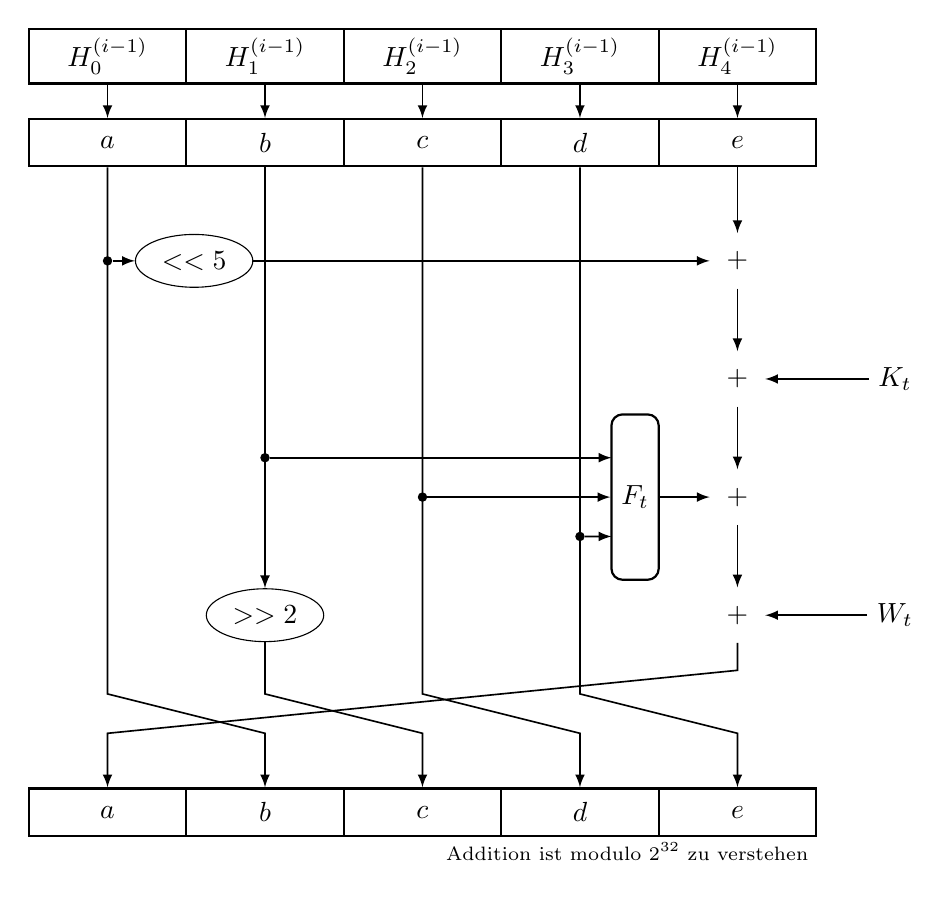
\begin{tikzpicture}
			\begin{scope}[>=latex] %for filled arrow tips
			\newcommand{\n}{5}
			
			\pgfmathsetmacro\minBoxWidth{(2.0)} // 2.2 old
			\pgfmathsetmacro\minBoxHeight{(0.6)} // 0.5 old
			
			\pgfmathsetmacro\xA{int(0)}
			\pgfmathsetmacro\xB{(\minBoxWidth * 1)}
			\pgfmathsetmacro\xC{(\minBoxWidth * 2)}
			\pgfmathsetmacro\xD{(\minBoxWidth * 3)}
			\pgfmathsetmacro\xE{(\minBoxWidth * 4)}
			
			\node (h0) at (\xA, {(\n -1)*2 + 2}) [draw,thick,minimum width=\minBoxWidth cm, minimum height=\minBoxHeight cm] {$H_0^{(i-1)}$};
			\node (h1) at (\xB, {(\n -1)*2 + 2}) [draw,thick,minimum width=\minBoxWidth cm, minimum height=\minBoxHeight cm] {$H_1^{(i-1)}$};
			\node (h2) at (\xC, {(\n -1)*2 + 2}) [draw,thick,minimum width=\minBoxWidth cm, minimum height=\minBoxHeight cm] {$H_2^{(i-1)}$};
			\node (h3) at (\xD, {(\n -1)*2 + 2}) [draw,thick,minimum width=\minBoxWidth cm, minimum height=\minBoxHeight cm] {$H_3^{(i-1)}$};
			\node (h4) at (\xE, {(\n -1)*2 + 2}) [draw,thick,minimum width=\minBoxWidth cm, minimum height=\minBoxHeight cm] {$H_4^{(i-1)}$};
			
			\pgfmathsetmacro\abcdeLineYCoord{(\n -1)*2 + 0.9}
			
			\node (a) at (\xA, \abcdeLineYCoord) [draw,thick,minimum width=\minBoxWidth cm, minimum height=\minBoxHeight cm] {$a$};
			\node (b) at (\xB, \abcdeLineYCoord) [draw,thick,minimum width=\minBoxWidth cm, minimum height=\minBoxHeight cm] {$b$};
			\node (c) at (\xC, \abcdeLineYCoord) [draw,thick,minimum width=\minBoxWidth cm, minimum height=\minBoxHeight cm] {$c$};
			\node (d) at (\xD, \abcdeLineYCoord) [draw,thick,minimum width=\minBoxWidth cm, minimum height=\minBoxHeight cm] {$d$};
			\node (e) at (\xE, \abcdeLineYCoord) [draw,thick,minimum width=\minBoxWidth cm, minimum height=\minBoxHeight cm] {$e$};
			
			\draw[->,semithick] (h0) -- (a);
			\draw[->,semithick] (h1) -- (b);
			\draw[->,semithick] (h2) -- (c);
			\draw[->,semithick] (h3) -- (d);
			\draw[->,semithick] (h4) -- (e);
			
			\pgfmathsetmacro\numAddBoxes{int(4)}
			\pgfmathsetmacro\lastAddBoxIndex{int(\numAddBoxes)}
			\pgfmathsetmacro\firstAddBoxYCoord{\abcdeLineYCoord - 1.5}
			
			%\node (plus0)[circle, draw] at (\xE,\firstAddBoxYCoord) {$+$};
			
			\foreach \nr in {1, ..., \numAddBoxes}{
				\node (plus\nr)[circle] at (\xE,{\abcdeLineYCoord - (1.5 * \nr)}) {$+$};
			}	
			
			\pgfmathsetmacro\lastAddBoxYCoord{\abcdeLineYCoord - 1.5 * \numAddBoxes}
			\draw[->,semithick] (e) -- (plus1);
			
			\foreach \nr in {1, ..., 3}{
				\pgfmathsetmacro\cnr{int(\nr + 1)}
				\draw[->,semithick] (plus\nr) -- (plus\cnr);
			}
			
			%draw Key and Message arrow
			\node (KeyArrow) at (\xE + 2.0, {\abcdeLineYCoord - (1.5 * 2)}) {$K_t$};
			\draw[->, semithick] (KeyArrow) -- (plus2);
			
			\node (MessageArrow) at (\xE + 2.0, {\abcdeLineYCoord - (1.5 * 4)}) {$W_t$};
			\draw[->, semithick] (MessageArrow) -- (plus4);
			
			\node (shiftL5)[ellipse, draw] at (\minBoxWidth * 0.5 + 0.1, \firstAddBoxYCoord) {$<< 5$};
			
			\node (p1)[circle, fill, inner sep=0cm, minimum size=0.12cm] at (\xA, \firstAddBoxYCoord) {};
			\draw[->, semithick] (p1) -- (shiftL5);
			\draw[->, semithick] (shiftL5) -- (plus1);
			
			\node (shiftR2)[ellipse, draw] at (\xB, \lastAddBoxYCoord) {$>> 2$};
			\draw[->, semithick] (b) -- (shiftR2);
			
			\node (rectF)[draw,thick,rounded corners,minimum width=0.6cm, minimum height=2.1cm] at (\xD + 0.7, {\abcdeLineYCoord - (1.5 * 3)}) {$F_{t}$};
			\node (p2)[circle, fill, inner sep=0cm, minimum size=0.12cm] at (\xC, {\abcdeLineYCoord - (1.5 * 3)}) {};
			\draw[->, semithick] (p2) |- (rectF);
			\draw[->, semithick] (rectF) -- (plus3);
			
			\node (p3)[circle, fill, inner sep=0cm, minimum size=0.12cm] at (\xB, {\abcdeLineYCoord - (1.5 * 3) + 0.5}) {};
			\draw[->, semithick] (p3) -- ($(rectF) + (-0.3, 0.5)$);
			
			\node (p4)[circle, fill, inner sep=0cm, minimum size=0.12cm] at (\xD, {\abcdeLineYCoord - (1.5 * 3) - 0.5}) {};
			\draw[->, semithick] (p4) -- ($(rectF) + (-0.3, -0.5)$);
			
			
			\node (aNew) at (\xA, {\lastAddBoxYCoord - 2.5}) [draw,thick,minimum width=\minBoxWidth cm, minimum height=\minBoxHeight cm] {$a$};
			\node (bNew) at (\xB, {\lastAddBoxYCoord - 2.5}) [draw,thick,minimum width=\minBoxWidth cm, minimum height=\minBoxHeight cm] {$b$};
			\node (cNew) at (\xC, {\lastAddBoxYCoord - 2.5}) [draw,thick,minimum width=\minBoxWidth cm, minimum height=\minBoxHeight cm] {$c$};
			\node (dNew) at (\xD, {\lastAddBoxYCoord - 2.5}) [draw,thick,minimum width=\minBoxWidth cm, minimum height=\minBoxHeight cm] {$d$};
			\node (eNew) at (\xE, {\lastAddBoxYCoord - 2.5}) [draw,thick,minimum width=\minBoxWidth cm, minimum height=\minBoxHeight cm] {$e$};
			%\draw[->, semithick] (shiftL5) -- (plus1);
			
			\draw[->, semithick] (a) -- (\xA, {\lastAddBoxYCoord - 1.0}) 
			-- (\xB, {\lastAddBoxYCoord - 1.5}) -- (bNew);
			
			\draw[->, semithick] (shiftR2) -- ($(shiftR2) + (0, -1)$) 
			-- (\xC, {\lastAddBoxYCoord - 1.5}) -- (cNew);
			
			\draw[->, semithick] (c) -- (\xC, {\lastAddBoxYCoord - 1.0}) 
			-- (\xD, {\lastAddBoxYCoord - 1.5}) -- (dNew);
			
			\draw[->, semithick] (d) -- (\xD, {\lastAddBoxYCoord- 1.0}) 
			-- (\xE, {\lastAddBoxYCoord - 1.5}) -- (eNew);
			
			\draw[->, semithick] (plus\lastAddBoxIndex) -- (\xE, {\lastAddBoxYCoord- 0.7}) 
			-- (\xA, {\lastAddBoxYCoord - 1.5}) -- (aNew);
			
			\node (AddModText) at (\xE - 1.4, {\lastAddBoxYCoord - 3.0}) {\scriptsize{Addition ist modulo $2^{32}$ zu verstehen}};
			
			\end{scope}
			\end{tikzpicture}
			\caption{Schema der Berechnungsrunde}
		\end{figure}
		\item Setze $H_0^{(i)} = H_0^{(i-1)} + a, \dots, H_4^{(i)} = H_4^{(i-1)} + e$.
	\end{enumerate}
	\item Gebe $H_0^{(n)} \concat \dots \concat H_4^{(n)}$ als 160-Bit Hashwert (\textit{message digest}) aus.
\end{enumerate} 

In jeder der 80 Berechnungsrunden zum Berechnen eines Zwischenergebnisses werden folgende Funktionen, Konstanten und Variablen verwendet:
\begin{itemize}
	\item Rundenfunktion $F_{t}$ führt, je nach Index, unterschiedliche Elementaroperationen auf den 32-Bit langen Variablen $b, c, d$ aus.
	\item Konstante $K_{t}$ hat, je nach Index, vier verschiedene Werte.
	\item Variable $W_{t}$, als \textit{message schedule} bezeichnet, besteht in den ersten 16 Runden jeweils aus einem 32-Bit Wort des aktuellen 512-Bit großen Nachrichtenblocks $\plaint_{i}$ und in den verbleibenden 64 Runden aus einem rekursiv berechneten Wert vergangener message schedules des gleichen Blocks.
\end{itemize}

Für die Eingangs erwähnten Angriffe auf die beschriebene Konstruktion wird die Möglichkeit ausgenutzt, für eine Runde Kollisionen zu finden und versucht, diese auf mehrere Runden auszuweiten. Dabei sind auch ähnliche Ausgaben hilfreich. Der schnellste der im Jahr 2005 vorgestellten Algorithmen benötigt mit ungefähr $2^{63}$-Schritten (vgl. $2^{80}$-Schritte für einen Brute-Force-Angriff) zwar noch immer einen beträchtlichen Rechenbedarf, erzeugt jedoch Kollisionen über alle 80 Berechnungsrunden.

Neben SHA-1 ist der im Jahr 1992 von Ronald Rivest veröffentlichte MD5-Algorithmus eine bekannte Hashfunktion, die auf dem Merkle-Damgård-Konstrukt beruht und für eine Vielzahl kryptographischer Anwendungen und Datenintegritäts-Sicherung eingesetzt wurde. Von der Verwendung von MD5 sollte für sicherheitsrelevante Anwendungsszenarien mittlerweile jedoch abgesehen werden: Im Unterschied zu SHA-1 können bei MD5 explizite Kollisionen gefunden werden. Im Jahr 2013 stellten Xie Tao, Fanbao Liu und Dengguo Feng den bis dato besten Angriff vor, der aus einer Menge von etwa $2^{18}$ MD5 Hashwerten ein Kollisionspaar findet. Heutige Prozessoren benötigen dafür weniger als eine Sekunde.
%fact check mit Hofheinz

Aufgrund der Verwundbarkeit von MD5 und SHA-1 empfiehlt die NIST
heutzutage mindestens eine Hashfunktion der SHA-2-Familie zu
verwenden. Ähnlich zu SHA-1 basieren die Funktionen dieser Hash-Familie
auf der Merkle-Damgård-Konstruktion, bieten jedoch in der Praxis,
aufgrund des größeren Bildraums, ein höheres Maß an
Sicherheit. Theoretisch aber bleiben die Funktionen, wegen großen
Ähnlichkeiten in der Konstruktion, verwundbar. Deshalb wurde im Jahr
2013 mit SHA-3 (\glqq Keccak\grqq{}-Algorithmus) der Versuch gestartet,
eine grundlegend andere kryptographische Hashfunktion zu
standardisieren. Dieser Standardisierungsprozess wurde am 05.08.2015 mit
der Veröffentlichung des NIST\footnote{Das Abschlussdokument findet sich
unter \url{https://www.federalregister.gov/articles/2015/08/05/2015-19181/announcing-approval-of-federal-information-processing-standard-fips-202-sha-3-standard}} abgeschlossen\footnote{Die Übersicht über den Standardisierungsprozess findet sich auf \url{http://csrc.nist.gov/groups/ST/hash/sha-3/sha-3_standardization.html}.}.

\section{Angriffe auf Hashfunktionen}
\subsection{Birthday-Attack}
Für diesen Angriff berechnen wir möglichst viele $Y_i = H(X_i)$.
Danach suchen wir unter diesen Hashwerten nach Gleichheit (und finden so $X \not = X'$ mit $H(X) = Y = Y' = H(X')$).
\vspace{10pt}

\textbf{Vorgehen:}
\begin{enumerate}
  \item Schreibe $(X_i, Y_i)$ in Liste. Dabei ist $X_i \in \{0,1\}^{2k}$ gleichverteilt und $Y_i = H(X_i)$.
  \item Sortiere die Liste nach $Y_i$.
  \item Untersuche die Liste auf $Y_i$-Kollisionen.
\end{enumerate}
\vspace{10pt}

\begin{theorem}
Sei $n \leq 2^{\frac{k}{2}}$ und $Y_1, \ldots , Y_n \in \{0,1\}^k$ unabhängig gleichverteilt. Dann gibt es $i \not = j$ mit $Y_i = Y_j$ mit Wahrscheinlichkeit
$p > \frac{1}{11} \cdot \frac{n^2}{2^k}$.
\end{theorem}
\vspace{10pt}
\begin{beweis}
  ohne Beweis
\end{beweis}
Wir haben also schon für $n = 2^{\frac{k}{2}}$ zufällige, verschiedene $X_i$ mit einer Wahrscheinlichkeit von $p > \frac{1}{11}$ Kollisionen unter den
den dazugehörigen $Y_i$. Für die Berechnung brauchen wir $\Theta(k \cdot 2^{\frac{k}{2}})$ Schritte und haben einen Speicherbedarf von $\Theta(k \cdot
2^{\frac{k}{2}})$ Bits.

\subsection{Weitere Angriffe}
Auch ein Meet-in-the-Middle-Angriff kann die Zeit zum Auffinden einer Kollision verkürzen. Allerdings setzt dieser Angriff voraus, dass die
Hashfunktion eine "`Rückwärtsberechnung"' zulässt.
\paragraph*{Angriffsbeschreibung}
\begin{itemize}
	\item Gegeben: $M = (M_1,\dots,M_n), H(M), i$.
	\item Gesucht: $M' = (M'_1,\dots,M'_n) \neq M$, so dass $H(M') = H(M)$.
	\begin{enumerate}
		\item Teile $M$ in Substrings $P = (M_1,\dots,M_i)$ und $S = (M_{i+1},\dots,M_{n})$.
		\item Berechne für jedes $P' = (M'_1,\dots,M'_i)$ den Wert $Z = H(P')$.
		\item Sortiere die Liste aller $Z$, um binäre Suche zu ermöglichen.
		\item Rechne ausgehend von $H(M)$ für ein $S' = (M'_{i+1},\dots,M'_{n})$ zu $Z'$ zurück.
		\begin{enumerate}
			\item Falls $Z'$ in der Liste aller $Z$ enthalten ist und das entsprechende $P' \neq P$ oder $S' \neq S$, dann haben wir eine Kollision für $M$ mit $M' = P' \concat S'$ gefunden.
			\item Wiederhole den Schritt ansonsten für ein anderes $S'$.
		\end{enumerate}
	\end{enumerate}
\end{itemize}
Der Aufwand für diesen Angriff nähert sich asymptotisch dem für die Geburtstagsattacke an.

\begin{figure}[h]
	\centering
	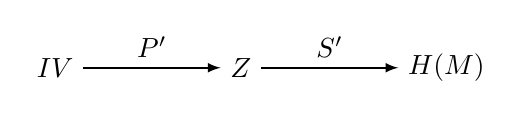
\begin{tikzpicture}[>=latex]		
		\node[anchor=east] (IV) at (0, 0) {$IV$};
		\node (Z) at (2, 0) {$Z$};
		\node[anchor=west] (H) at (4, 0) {$H(M)$};
		
		\draw[->, semithick] (IV.east) -- (Z.west) node[above, pos=.5]{$P'$};
		\draw[->, semithick] (Z.east) -- (H.west) node[above, pos=.5]{$S'$}; 
	\end{tikzpicture}
	\caption{Hilfsskizze für Meet-in-the-Middle-Angriff auf eine Hashfunktion $H$}
	\label{fig:md-meet-in-the-middle-attack}
\end{figure}

%\begin{figure}[h]
%\begin{center}
%\unitlength=1mm
%\linethickness{0.4pt}
%\hspace{-3 cm}
%\begin{picture}(50,10)
%
%\put(0,2){\makebox(0,0)[cb]{$IV$}}
%
%\put(5,3){\vector(1,0){15}}
%\put(12,4){\makebox(0,0)[cb]{$P'$}}
%
%\put(20,0.5){\makebox(10,5){$Z$}}
%
%\put(30,3){\vector(1,0){15}}
%\put(37,4){\makebox(0,0)[cb]{$S'$}}
%
%\put(47,0.5){\makebox(10,5){$H(M)$}}
%
%\end{picture}
%\end{center}
%\caption{Hilfsskizze für Meet-in-the-Middle-Angriff auf eine Hashfunktion $H$}
%\label{fig:md-meet-in-the-middle-attack}
%\end{figure}

\subsection{Fazit}
Die vorgestellten Angriffe zeigen, dass sich der Aufwand zum Finden einer Kollision gegenüber einer Brute-Force-Attacke stark verringern lässt. Bei einer
Hash-Ausgabe mit einer Länge $\geq k$ Bits kann man nur mit einer "`Sicherheit"' von $\frac{k}{2}$ Bits rechnen.

\chapter{Asymmetrische Verschlüsselung}
\label{ch:asymmenc}

Symmetrische Verschlüsselung, wie wir sie in den letzten Kapiteln behandelt haben, funktioniert über ein gemeinsames Geheimnis $K$ (siehe Abbildung
%\ref{fig:symmenc}).
).
Das verursacht uns einige Unannehmlichkeiten:

\begin{itemize}
  \item das gemeinsame Geheimnis $K$ muss auf einem sicheren Kanal übertragen werden.
  \item bei $n$ Benutzern werden im System $\binom{n}{2} = \frac{n \cdot (n-1)}{2}$ Schlüssel verwendet (für jedes Teilnehmerpaar einen).
\end{itemize}

%\includesvg[width=\textwidth]{images/vergleich-symmetrisch-asymmetrisch}
%\begin{figure}[h]



%\begin{center}
%\unitlength=1mm
%\linethickness{0.4pt}
%\hspace{-3 cm}

%\begin{picture}(30,10)
%\put(0,2){\makebox(0,0)[cb]{$\text{Alice}_K$}}
%\put(50,3){\vector(-1,0){40}}
%\put(30,4){\makebox(0,0)[cb]{$C := \text{Enc}(K, M)$}}
%\put(55,0.5){\makebox(10,5){$\text{Bob}_K$}}
%\end{picture}
%#\end{center}
%caption{Schematischer Ablauf einer symmetrisch verschlüsselten Kommunikation}
%\label{fig:symmenc}
%\end{figure}


\section{Idee}
Asymmetrische Verschlüsselung, auch \emph{Public-Key-Kryptographie}
genannt,  basiert auf der Grundidee, für die Verschlüsselung
(öffentlich) einen anderen Schlüssel zu verwenden als für die
Entschlüsselung (privat).

Die Vorteile eines Public-Key-Verfahrens sind offensichtlich. Wir
benötigen für den Schlüsselaustausch keinen sicheren Kanal mehr, sondern
könnten sogar ähnlich einem Telefonbuch ein öffentliches Verzeichnis mit
den öffentlichen Schlüsseln anlegen. Außerdem müssen nicht mehr so viele
Schlüssel gespeichert werden: Bei $n$ Benutzern gibt es nur noch $n$
öffentliche (und $n$ geheime) Schlüssel. 

Die Sicherheit eines solchen Verfahrens hängt davon ab, wie schwierig es
für einen Angreifer ist, vom (allgemein bekannten) öffentlichen
Schlüssel $pk$ auf den (geheim gehaltenen) privaten Schlüssel $sk$ zu
schließen. Um das praktisch unmöglich zu machen, greift man auf Probleme
zurück, die nach aktuellem Forschungsstand nicht effizient lösbar
sind. Im Folgenden werden zwei Verfahren vorgestellt, die asymetrische
Verschlüsselung basierend auf dem RSA-Problem bzw. dem DLOG-Problem
konstruieren. 
% \begin{figure}[h]
% \begin{center}
% \unitlength=1mm
% \linethickness{0.4pt}
% \hspace{-3 cm}
% \begin{picture}(30,10)
% \put(0,2){\makebox(0,0)[cb]{$\text{Alice}_{sk}$}}
% \put(50,3){\vector(-1,0){40}}
% \put(30,4){\makebox(0,0)[cb]{$C := \text{Enc}(pk, M)$}}
% \put(55,0.5){\makebox(10,5){$\text{Bob}_{pk}$}}
% \end{picture}
% \end{center}
% \caption{Schematischer Ablauf einer asymmetrisch verschlüsselten Kommunikation}
% \label{fig:asymmenc}
% \end{figure}

\begin{figure}
\includegraphics[width=\textwidth]{images/vergleich-symmetrisch-asymmetrisch.eps}
\caption{Unterschiede in der Vorbereitung von symmetrisch und
  asymmetrisch verschlüsselter Kommunikation}
\label{fig:asymmenc-symmenc}
\end{figure}
Damit Bob eine asymmetrisch verschlüsselte Nachricht an Alice senden
kann, benötigt er ihren öffentlichen Schlüssel. Dieser darf
unverschlüsselt verschickt werden, es muss aber sichergestellt werden,
dass der Schlüssel nicht bei der Kommunikation manipuliert wurde. Dies
geschieht über eine sogenannte \textit{Public Key Infrastructure}, was
hier jedoch nicht weiter vertieft wird.
\section{Sicherheitsbegriffe für asymmetrische Verfahren}
Die Sicherheitsbegriffe, die wir in Kapitel \ref{chap:krypt-begriffe}
kennen gelernt haben, finden mit leicht abgewandelten Definitionen auch
bei asymmetrischen Verfahren Anwendung:

\begin{definition}[Semantische Sicherheit für Public-Key-Verfahren]
Ein Pub\-lic-""Key-""Ver\-schlüs\-sel\-ungs\-sche\-ma ist \textit{semantisch sicher}, wenn es für jede $M$-Verteilung von Nachrichten gleicher Länge, jede
Funktion $f$ und jeden PPT-Algorithmus $\A$ einen PPT-Algorithmus $\B$ gibt, so dass
\begin{equation*}
\Pr\left[\A(1^k, pk, \enc(pk, M)) = f(M)\right] - \Pr\left[\B(1^k) = f(M)\right]
\end{equation*}
vernachlässigbar (als Funktion im Sicherheitsparameter) ist.
\end{definition}

\begin{definition}[IND-CPA-Sicherheit für Public-Key-Verfahren]
  Betrachte folgendes Experiment mit einem Herausforderer $\C$ und einem
  PPT-Angreifer $\A$. $\C$ generiert mit dem Generator-Algorithmus ein
  Schlüsselpaar $(pk, sk)$. $\A$ erhält zu Beginn $pk$.
  \begin{itemize}
  \item $\A$ kann sich zu jedem Zeitpunkt jedes beliebige $\plaint$
    mithilfe von $pk$ verschlüsseln.
  \end{itemize}
  \begin{enumerate}
  \item $\A$ wählt zwei Nachrichten $\plaint_1$, $\plaint_2$ gleicher
    Länge.
  \item $\A$ erhält $\ciphert^{*} := \enc(pk, \plaint_{b})$ für ein von
    $\C$ zufällig gleichverteilt gewähltes $b \in \{1, 2\}$.
  \item $\A$ gewinnt, wenn er $b$ korrekt errät.
  \end{enumerate} 
  Ein asymmetrisches Verfahren $(\gen, \enc, \dec)$ heißt IND-CPA-sicher, wenn der Vorteil des
  Angreifers gegenüber dem Raten einer Lösung, also $\Pr \left[ \A
    \textnormal{ gewinnt} \right] - \frac{1}{2}$, für alle
  PPT-Algorithmen $\A$ vernachlässigbar im Sicherheitsparameter $k$ ist.
\end{definition}

Der IND-CPA-Begriff unterscheidet sich also dadurch vom symmetrischen
Fall, dass ein Angreifer $\A$ kein Orakel mehr braucht, sondern
Chiffrate selbst mit dem öffentlichen Schlüssel erzeugen kann.

Auch IND-CCA hat eine Variante für asymmetrische Verfahren, die wir aber
nicht weiter vertiefen.

\section{RSA}
Das bekannteste Public-Key-Verfahren ist RSA (1977). Es ist benannt nach seinen
Erfindern Ronald Rivest, Adi Shamir und Leonard Adleman.

\subsection{Erweiterter Euklidischer Algorithmus}
\label{ssec:eea}
Um das Vorgehen der Schlüsselerzeugung des RSA-Algorithmus erklären zu
können, führen wir den \emph{Erweiterten Euklidischen Algorithmus} (EEA)
als Hilfskonstrukt ein, der es uns erlaubt, das inverse Element $t$ zu
$B$ über einer multiplikativen Gruppe $\mathbbm{Z}^{\ast}_{A}$ zu
bestimmen. Für gegebene Parameter $A$ und $B$ berechnet der EEA neben
dem größten gemeinsamen Teiler $\ggT(A, B)$ zwei ganze Zahlen $s$ und $t$, sodass 

\begin{align*}
	\ggt(A, B) = s \cdot A + t \cdot B\, .
\end{align*}

Für das RSA-Verfahren reicht es, den Spezialfall $\ggT(A,B) = 1$ zu betrachten, der folgenden Zusammenhang liefert:

\begin{align*}
	1 &= s \cdot A + t \cdot B\\
	\Leftrightarrow 1 &\equiv t \cdot B \pmod A
\end{align*}

Bezüglich $\mathbbm{Z}^*_{A}$ ist $t$ also das zu $B$
multiplikativ-inverse Element. Das Vorgehen betrachten wir beispielhaft
für $B = 23$, zu dem das inverse Element über $\mathbbm{Z}^{\ast}_{192}$
bestimmt werden soll.

Wir betrachten im Folgenden zwei Varianten des erweiterten Euklidischen
Algorithmus.

Der EEA entwickelt zwei Variablen $s$ und $t$ iterativ, sodass gilt: 
    \begin{align*}
      s_{i+1} &= s_{i-1} - f_{i+1} \cdot s_{i}\\
      t_{i+1} &= t_{i-1} - f_{i+1} \cdot t_{i}
    \end{align*}
Hierbei ist $f_i = \max \{f : f \cdot B_i \leq A_i\}$ und die größte
Zahl, die  $R_i > 0$
%\begin{subsubsection}[EEA mit Vorwärts-Entwicklung]
  \begin{beispiel}[EEA]
    Es sei $A = A_2 = 192 $ und $B = B_2 = 23$. Es ist offensichtlich $\ggT(192, 23) = 1$, da B prim ist. Nun berechnen wir ausgehend von $i = 2$ in
    \begin{align*}
      A_i = f_i \cdot B_i + R_i
    \end{align*}
    jeweils $f_i = \max \{f : f \cdot B_i \leq A_i\}$ und $R_i > 0$, bis
    $R_i = 0$. Dabei ist $A_{i+1} = B_i$ und $B_{i+1} = R_i$. Parallel
    dazu entwickeln wir die Parameter $s$ und $t$ über die Gleichungen 
    \emph{vorwärts}. Wir erhalten demnach
    \begin{table}[h]
      \centering
      \large
      \begin{tabular}[c]{|c|l|rrr|l|}
        \hline
        & Gleichung & $R_i$ & $s_i$ & $t_i$ &\\
        \hline
        \hline
        (0) & $192 = 1 \cdot 192 + 0 \cdot 23$ & $192$ & $1$ & $0$ &\\
        (1) & $23 = 0 \cdot 192 + 1 \cdot 23$ & $23$ & $0$ & $1$ &\\
        \hline 
        & EEA & & & &\\
        \hline
        (2) & $192 = 8 \cdot 23 + 8$ & $8$ & $1$ & $-8$ & $\text{(0)} - 8 \cdot \text{(1)}$\\
        (3) & $23 =  2 \cdot 8 + 7$ & $7$ & $-2$ & $17$ & $\text{(1)} - 2 \cdot \text{(2)}$\\
        (4) & $8 = 1 \cdot 7 + 1$ & $1$ & $3$ & $-25$ & $\text{(2)} - 1 \cdot \text{(3)}$\\ 
        (5) & $7 = 7 \cdot 1 + 0$ & $0$ & $-23$ & $192$ & $\text{(3)} - 7 \cdot \text{(4)}$\\
        \hline
      \end{tabular}
    \end{table}
    \subsubsection*{Varianten 1: Vorwärts-Entwicklung}
    Die vom EEA berechneten Werte, das heißt die Parameter $s$ und $t$, stehen in der (4). Zeile. Es ist also 
    \begin{align*}
      1 &= 3 \cdot 192 + (-25) \cdot 23\\
      \Leftrightarrow 1 &\equiv (-25) \cdot 23 \pmod{192}\\
      \Leftrightarrow 1 &\equiv (192 - 25) \cdot 23 \pmod{192}\\ 
      \Leftrightarrow 1 &\equiv 167 \cdot 23 \pmod{192}\, \text{,}
    \end{align*}
    und somit $167$ das zu $23$ multiplikativ-inverse Element bezüglich
    $\mathbbm{Z}^{\ast}_{192}$.
    \subsubsection*{Varianten 2: Rückwärts-Entwicklung}
    Ebenso ist es möglich, die Parameter $s$ und $t$ \emph{rückwärts} zu berechnen. Dazu werden, ausgehend von (2), 
    die Gleichungen (3), (4) und (5) aufgestellt und anschließend wie folgt ineinander eingesetzt:  
    \begin{align*}
      \begin{split}
        1	&\stackrel{\textit{(4)}}{=} 8 - 1 \cdot 7\\
        &\stackrel{\textit{(3)}}{=} 8 - 1 \cdot (23 - 2 \cdot 8) = -23 + 3 \cdot 8\\
        &\stackrel{\textit{(2)}}{=} -23 + 3 \cdot (192 - 8 \cdot 23) = 3 \cdot 192 - 25 \cdot 23\\[.5cm]
        &\equiv -25 \cdot 23 \pmod{192}\\
        &\equiv 167 \cdot 23 \pmod{192}
      \end{split}
    \end{align*}
  \end{beispiel}
%\end{subsubsection}
%\begin{subsubsection}[EEA mit Rückwärts-Entwicklung]
  
%\end{subsubsection}

\subsection{Vorgehen}
\label{ch:asymmenc:rsa:vorgehen}
Um RSA nutzen zu können, brauchen wir drei Algorithmen: Einen
Generator-Algorithmus $\operatorname{Gen}$, einen
Verschlüsselungsalgorithmum $\operatorname{Enc}$ und einen
Entschlüsselungsalgorithmus $\operatorname{Dec}$.
\subsubsection{Generator-Algorithmus}
Für die Erstellung eines Schlüsselpaares werden zwei große Primzahlen benötigt. Die Berechnung des öffentlichen und privaten Schlüssels funktioniert folgendermaßen:
\begin{itemize}
 	\item Wähle zwei große Primzahlen $P, Q$ mit $P \neq Q$ und vorgegebener Bitlänge $k$.
 	\item Berechne $N = P \cdot Q$.
 	\item Berechne $\varphi(N) = (P - 1)(Q - 1)$\footnote{$\varphi$
            bezeichnet die Eulersche Phi-Funktion. Sie gibt für jede
            natürliche Zahl n an, wie viele zu n teilerfremde natürliche
            Zahlen es gibt, die nicht größer als n sind: 
            $\varphi(n) := \vert \{a\in\N \, |\, 1 \le a \le n
            \land \operatorname{ggT}(a,n) = 1 \} \vert$. Insbesondere
            ist $\varphi(N)$ die Anzahl multiplikativ invertierbarer
            Elemente im Restklassenring $\mathbb{Z}/N\mathbb{Z}$.
            Sie ist multiplikativ, d.h. es gilt für teilerfremde $n$, $m$:
            $\varphi(m\cdot n) = \varphi(m) \cdot \varphi(n)$. Da eine
            Primzahlen $p$ nur durch 1 und sich selbst teilbar ist, 
            gilt $\varphi(p) = p-1$. Somit gilt für zwei Primzahlen $p$,
            $q$ also $\phi(p \cdot q) = \phi(p) \cdot \phi(q) = (p-1)(q-1)$.}.
 	\item Wähle $e \in \{3, \dotsc, \varphi(N) - 1\}$, wobei $\ggT(e, \varphi(N)) = 1$.
 	\item Berechne mit Hilfe des \hyperref[ssec:eea]{EEA} das zu $e$ multiplikativ-inverse Element $d$ bezüglich $\varphi(N)$, d.h. $d \equiv e^{-1} \pmod{\varphi(N)}$.
\end{itemize}

Damit ist der geheime Schlüssel $sk = (N, d)$ und $pk = (N, e)$ der
öffentliche Schlüssel. Üblicherweise werden $P$ und $Q$ zufällig
gleichverteilt aus den ungeraden Zahlen der Bitlänge $k$ gezogen, bis
$P$ und $Q$ prim sind. Der Nachrichtenraum ist \Z{N}. 
\subsubsection{Ver- und Entschlüsselung}
Für die Ver- und
Entschlüsselungsfunktion gilt: 
\begin{align*}
	\enc(pk, M) & = M^e \mod N \\
	\dec(sk, C) & = C^d \mod N  
\end{align*}

Wie immer muss $\dec(\enc(M)) = M$ gelten. Für die Korrektheit von RSA bedeutet das, dass
\begin{align*}
	(M^e)^d \equiv M^{ed} \equiv M \pmod N
\end{align*}
erfüllt sein muss. Um das zu beweisen, verwenden wir den Kleinen Satz von Fermat und den Chinesischen Restsatz.
\begin{theorem}[Kleiner Satz von Fermat]
Für primes $P$ und $M \in \{1, \dotsc, P-1\}$ gilt: $M^{P-1} \equiv 1 \mod P$.
\end{theorem}
\begin{beweis}
  ohne Beweis
\end{beweis}
Daraus folgt auch: $\forall M \in \Z P, \alpha \in \mathbbm{Z} : (M^{P-1})^{\alpha} \cdot M \equiv M \mod P$.

\begin{theorem}[Chinesischer Restsatz]
Sei $N = P \cdot Q$ mit $P, Q$ teilerfremd. Dann ist die Abbildung $\mu : \Z N \rightarrow \Z P \times \Z Q$ mit $\mu(M) \equiv (M \mod P, M \mod Q)$ bijektiv.
\end{theorem}
\begin{beweis}
  ohne Beweis
\end{beweis}
Daraus folgt auch: $(X \equiv Y \mod P) \land (X \equiv Y \mod Q) \Rightarrow X \equiv Y \mod N$.

\begin{theorem}[Korrektheit von RSA]
Sei $N = P \cdot Q$ mit $P, Q$ teilerfremd und prim. Seien weiter $e, d$ teilerfremd wie oben. Dann ist $M^{ed} \equiv M \mod N$ für alle $M \in \Z N$.
\end{theorem}

\begin{beweis}
Nach Definition gilt $e \cdot d \equiv 1 \mod (P-1)(Q-1)$. Daraus folgt:
\begin{align*}
(P-1)(Q-1) \mid ed - 1 \quad
& \Rightarrow \quad P-1 \mid ed - 1\\
& \Rightarrow \quad ed = \alpha (P-1) + 1 \quad (\text{für } \alpha \in \mathbbm{Z})\\
& \Rightarrow \quad M^{ed} = (M^{(P-1)})^{\alpha} \cdot M \stackrel{\text{Fermat}}\equiv M \mod P
\end{align*}
Analog ist $M^{ed} \equiv M \mod Q$.\\
Da $N = P \cdot Q$ ergibt sich mithilfe des Chinesischen Restsatzes:
\begin{align*}
(M^{ed} \equiv M \mod P) \land (M^{ed} \equiv M \mod Q) \Rightarrow M^{ed} \equiv M \mod N
\end{align*}
\qed
\end{beweis}

Das bisher behandelte Verfahren wird häufig \textit{Textbook-RSA} genannt und
umfasst das grundlegende Prinzip von RSA. Textbook-RSA weist einige
Schwächen auf, die im nächsten Kapitel genauer besprochen
werden. Deshalb sollte es in der Praxis nicht verwendet werden.

\subsection{Sicherheit von (Textbook-)RSA}
\label{ch:asymmenc:rsa:sicherheit}
Bevor wir die Sicherheit von RSA betrachten, benötigen wir einen Sicherheitsbegriff, an dem wir uns bei der Beurteilung von asymmetrischen
Verschlüsselungsverfahren orientieren können. Wir definieren semantische
Sicherheit, vergleichbar mit der Definition für symmetrische Chiffren in
Kapitel \ref{ch:sicherheitsbegriffe:semantischesicherheit} und
äquivalent zu IND-CPA. 

RSA ist deterministisch, d.h. eine Nachricht $M$ wird unter Verwendung
desselben Schlüssels $pk$ immer zum gleichen Chiffrat $C_M$
verschlüsselt. Dadurch kann ein PPT-Angreifer zwei Chiffrate (z.B. $\enc(pk, \text{annehmen})$ und $\enc(pk,
\text{ablehnen})$) effizient voneinander
unterscheiden. RSA ist also nicht IND-CPA-sicher (und damit auch
nicht semantisch sicher). 

Ein mathematisches Problem, dass eng mit der Sicherheit von RSA
verknüpft ist, ist die Faktorisierung von natürlichen Zahlen. Hierbei
geht es darum eine gegebene Zahl $N$ in seine Primzahlfaktoren zu
zerlegen. Zur Zeit ist kein Algorithmus bekannt, der das
Faktorisierungsproblem in Polynomialzeit löst. Wäre ein solcher
Algorithmus bekannt, so könnte man leicht RSA \glqq brechen\grqq , indem
man $N$ in $P$ und $Q$ faktorisiert und dann mit Hilfe des euklidischen
Algorithmus und dem öffentlichen Schlüssel den geheimen Schlüssel
berechnet. Umgekehrt ist jedoch nicht bekannt, ob ein Algorithmus der
RSA bricht \footnote{Im Sinne von schwächeren
Sicherheitsbegriffen. Unter gewissen mathematischen Annahmen (die nicht
mit der Faktorisierung zu verwechseln sind) kann man beispielsweise
zeigen, dass es schwierig ist, aus ei- nem gegebenen RSA-Chiffrat den
kompletten Klartext zu berechnen. Diese Sicherheitsbegriffe werden in
dieser Vorlesung aber nicht weiter thematisiert.} auch einen Algorithmus
impliziert, der das Faktorisierungsproblem effizient löst. Dies ist eine
wichtige offene Forschungsfrage der Kryptographie. \footnote{In der
gängigen populärwissenschaftlichen Literatur und Magazinen liest man
häufig Sätze wie \glqq RSA zu brechen is so schwierig wie
Faktorisieren\grqq dies ist, wie oben argumentiert, mit Vorsicht zu
genießen.}

Textbook-RSA hat noch einige andere
Angriffspunkte, die im Folgenden umrissen werden. 

\begin{description}
\item[Wahl von $e$:] Aus Effizienzgründen liegt es auf den ersten Blick
  nahe, den Parameter $e$ aus dem öffentlichen Schlüssel nicht für jeden
  Benutzer neu zu berechnen, sondern für alle gleich zu wählen. Da diese
  Wahl nur den öffentlichen Schlüssel betrifft, scheint diese
  Einschränkung nicht kritisch zu sein, führt jedoch zu Problemen, wenn
  dieselbe Nachricht $M$ an mehrere unterschiedliche Benutzer
  verschlüsselt gesendet wird. 
  
  Sei beispielsweise $e=3$. Ein PPT-Angreifer, der die drei öffentlichen
  Schlüssel $pk_1, pk_2, pk_3$ kennt, mit denen $M$ verschlüsselt wurde,
  kann sich die Nachricht $M$ berechnen. Hierzu verwendet man den
  chinesischen Restsatz:

  Es gibt ein $X$ mit
  \begin{align*}
    X \equiv M^3 \mod N_1\\
    X \equiv M^3 \mod N_2\\
    X \equiv M^3 \mod N_3\\
  \end{align*}
  und mit dem chinesischen Restsatz
  \begin{align*}
    X \equiv M^3 \mod N_1N_2N_3
  \end{align*}

Da $M < N_1, N_2, N_3$ gilt insbesondere $M^3<N_1N_2N_3$, also kann man nun die dritte Wurzel von $X$ in $\mathbbm{Z}$
berechnen und hat damit $M$ berechnet.
    % \begin{align*}
    %  & M^3 \mod N_i  && \text{für } 1 \leq i \leq 3\\
    % = & M^3 \mod N_1N_2N_3  && \text{(Chinesischer Restsatz)}\\
    % = & M^3 && (\text{wegen } 0 \leq M < N_1,N_2,N_3)
    % \end{align*}
    % Wurzelziehen über $\mathbbm{Z}$ liefert die Nachricht $M$.
    
\item[Wahl von $N$:] 
  Nutzen zwei Benutzer Schlüssel mit dem selben $N$, ergeben sich zwei
  weitere Angriffe:
  \begin{itemize}
  \item Wird wieder dieselbe Nachricht $M$ mit zwei
    öffentlichen Schlüsseln $(N, e_1)$ und $(N, e_2)$ chiffriert und
    gilt weiterhin $\text{ggT}(e_1, e_2) = 1$ in $\Z{}$, kann ein
    PPT-Angreifer aus den Chiffraten $M$ berechnen:
    \begin{alignat*}{2}
      re_1 + se_2 & = 1\\ 
      \Longrightarrow C_1^rC_2^s \mod N &= M^{re_1}M^{se_2} &\mod N\\
                  &= M^{re_1 + se_2} &\mod N\\
                  &= M &\mod N
    \end{alignat*}
  \item
    Ist $N$ für zwei Benutzer $A$, $B$ gleich, dann kennen beide Benutzer $P$ und
    $Q$, also auch $\varphi(N)$. Damit kann $A$ mit $pk_A = (N, e_A)$
    nun einfach ein $d_B'$ zu Benutzer $B$ mit $pk_B = (N, e_B)$
    berechnen mit 
    \[d_B'=e_B^{-1} \mod \varphi(N).\]
    Dies geht genauso wie die RSA-Schlüsselerzeugung.
  \end{itemize}    
\item[Homomorphie:] Auf der multiplikativen Gruppe $(\mathbbm{Z}, \cdot)$ des RSA-Modulus gilt der Zusammenhang
  \begin{alignat*}{2}
      \enc(pk, M_1) \cdot \enc(pk, M_2) &\equiv M_1^e \cdot M_2^e &
      \pmod N \\
      &\equiv (M_1 \cdot M_2)^e & \pmod N\\
      &\equiv \enc(pk, M_1 \cdot M_2) & \pmod N
  \end{alignat*}
  und wir sehen, dass RSA homomorph ist. 
  Folgendes Beispiel soll veranschaulichen, zu welchen Zwecken die Homomorphie wahkann:   
    \begin{beispiel}
    	Wir betrachten eine Auktion mit dem Auktionsleiter $A$ und zwei Bietern $B_1$ und $B_2$. Damit keiner der Interessenten einen
    	anderen knapp überbietet oder sich von den Geboten anderer in seiner eigenen Abgabe beeinflussen lässt, nimmt der Auktionator die Gebote verschlüsselt entgegen. Dafür hat er seinen öffentlichen Schlüssel $pk_A$ zur Verfügung gestellt. Das Gebot eines Bieters wird chiffriert und zur Aufbewahrung an den Auktionator geschickt. Wenn die Zeit abgelaufen ist, werden keine neuen Preisvorschläge mehr angenommen, die eingegangenen Gebote entschlüsselt und der Höchstbietende ermittelt.
    
    	Der unehrliche Bieter $B_2$ kann nun seinen Preisvorschlag mithilfe des verschlüsselten Gebots von $B_1$ zu seinen Gunsten wählen. Dafür setzt er z.B. $C_2 =
    	C_1 \cdot \enc({pk_A, 2})$ oder, wenn er besonders sparsam ist, $C_2 = C_1 \cdot \enc({pk_A, 1001/1000 \mod N})$. Damit kann er das Gebot von $B_1$ verdoppeln
    	bzw. knapp überbieten, ohne dass der Auktionator und der ehrliche Bieter $B_1$ ihm Betrug nachweisen können.
    \end{beispiel}
\end{description} 

\subsection{Sicheres RSA} Wir haben festgestellt, dass RSA
deterministisch und damit nicht semantisch sicher ist. Die gepaddete
Variante \emph{RSA optimal asymmetric encryption padding} (RSA-OAEP)
dagegen ist IND-CCA-sicher im \emph{Random Oracle Model}\footnote{Im
  Random Orcale Model geht man von einer idealisierten Form von
  Hashfunktionen aus, die in der Realität nicht existiert. Trotzdem wurde
  bisher kein in diesem Model als sicher bewiesenes Verfahren \glqq
  gebrochen\grqq. Die Bewertung des Random Orcale Models ist ein viel
  diskutiertes Thema, worauf hier aber nicht weiter eingegangen werden
  soll.}. Wir verwenden dabei eine Zufallszahl $R$, mit deren Hilfe wir
die Nachricht $M$ vor dem Verschlüsseln abwandeln. Zu diesem Zweck wird
die in Abbildung \ref{fig:rsa-oaep} dargestellte Konstruktion von
Hashfunktionen $G, H$ verwendet. $R$ muss nach dem Entschlüsseln
nicht gespeichert werden, da es sich mit $Y \oplus H(X)$ berechnen lässt,
aber $\enc_R(M)$ lässt sich nun nicht mehr so einfach mit anderen
Chiffraten abgleichen.

\begin{figure}[h]
    \begin{center}
    \unitlength=1mm
    \linethickness{0.4pt}
    \hspace{-3 cm}
        \begin{picture}(60,60)
        
        \put(0,50){\framebox(30,5){$m$}}
        \put(32,50){\framebox(15,5){$000$}}
        \put(55,50){\framebox(20,5){$R$}}
        
        \put(15,45){\line(0,1){5}}
        \put(39,45){\line(0,1){5}}
        \put(15,45){\line(1,0){24}}
        \put(25,45){\vector(0,-1){40}}
        
        \put(65,50){\vector(0,-1){45}}
                
        \put(45,35){\circle{7}}
        \put(45,34){\makebox(0,0)[cb]{$G$}}
        \put(25,35){\circle{4}}
        \put(23,35){\line(1,0){18.5}}
        \put(65,35){\vector(-1,0){16.5}}
        
        \put(45,20){\circle{7}}
        \put(45,19){\makebox(0,0)[cb]{$H$}}
        \put(65,20){\circle{4}}
        \put(25,20){\vector(1,0){16.5}}
        \put(48.5,20){\line(1,0){18.5}}
        
        \put(0,0){\framebox(45,5){$X$}}
        \put(55,0){\framebox(20,5){$Y$}}
            
        \end{picture}
    \end{center}
    \caption{Pad-Funktion von RSA-OAEP ($G,H$ sind Hashfunktionen)}
    \label{fig:rsa-oaep}
\end{figure}

\subsubsection{Verschlüsselung mit RSA-OAEP}
Um mit RSA-OAEP zu verschlüsseln, wendet man erst das Padding-Verfahren
aus Grafik \ref{fig:rsa-oaep} an und verschlüsselt danach mit RSA, wobei
das Schlüsselpaar wie bei RSA generiert wurde:
\begin{itemize}
\item Wähle $R$ zufällig.
\item Berechne
\begin{align*}
  X & = m \oplus G(R) \\
  Y & = R \oplus H(X).
\end{align*}
\item Verschlüssele gemäß:
\[
  \enc_{OAEP}(pk, M) = (X||Y)^e \mod N.
\]
\end{itemize}
\subsubsection{Entschlüsselung mit RSA-OAEP}
Zur Entschlüsselung eines Chiffrats $C$ wird erst RSA-Entschlüsselung
angewendet, danach wird das Padding rückgängig gemacht:
\begin{itemize}
\item Rekonsturiere $(X||Y) = \dec(sk, C)$.
\item rekonstruiere $R$ mit $R = Y \oplus H(X)$.
\item Berechne $M$ mit $M = X \oplus G(R)$.
\end{itemize}

\subsection{Bedeutung von RSA}
Im Gegensatz zu den meisten symmetrischen Chiffren basiert RSA als
Beispiel einer asymmetrischen Verschlüsselungstechnik nicht auf
einfachen, bit-orientierten sondern auf einer mathematischen
Funktion. Der für Ver- und Entschlüsselung, sowie für die
Schlüsselerzeugung nötige Rechenaufwand steigt dadurch ungemein: Ein
naiver Exponentiationsalgorithmus benötigt für die Berechnung einer
modulo $l$-Bit-Zahl $\omega(l)$ Bitoperationen. %TODO: Was ist ein
%Exponentiationsalgorithmus?

Nichtsdestotrotz wird RSA in der Praxis häufig eingesetzt. Es macht sich
relativ einfache Arithmetik zunutze und die Ähnlichkeit zwischen Ver-
und Entschlüsselungsfunktion vereinfachen die Implementierung
zusätzlich. Mit einfachen Anpassungen ($e = 3$ bei Verschlüsselung,
Chinesischer Restsatz nutzen bei Entschlüsselung) kann RSA so weit
beschleunigt werden, dass es die Laufzeit betreffend gegenüber anderen
Verschlüsselungsverfahren konkurrenzfähiger wird.

\section{ElGamal}
\label{ch:asymenc:elgamal} Das ElGamal-Verfahren (1985) macht sich die
Schwierigkeit zunutze, das DLOG-Problem, also die Berechnung von
diskreten Logarithmen in zyklischen Gruppen, zu lösen. Unter einer
zyklischen Gruppe versteht man eine Gruppe $\mathbbm{G}$, bei der ein
sogenanntes Erzeugerelement $g$ existiert, so dass $\mathbbm{G} =
\langle g \rangle := \{g^k \mid k \in \mathbbm{Z}\}$.

\subsection{Vorgehen} 
Für die Schlüsselerzeugung wird eine ausreichend große Gruppe
$\mathbbm{G}$ mit Primordnung $p$ mit dem Erzeuger $g$ verwendet. 
\subsubsection{Schlüsselerzeugung}
Zur Schlüsselerzeugung wird ein $x \in {2,\dots, p-1}$ zufällig gewählt
und $h \equiv g^x$ berechnet. Dann sind
\begin{align*}
pk &= (\mathbbm{G}, g, h)\\ 
sk &= (\mathbbm{G}, g, x)
\end{align*}

\subsubsection{Ver- und Entschlüsselung}
Es wird ein $y \in \mathbbm{G}$ zufällig gewählt. Ver- und Entschlüsselung sind dann definiert durch
\begin{align*} 
&\enc(pk, M) = (g^y, h^y \cdot M) \\ 
&\dec(sk, (g^y, C))
= \frac{C}{(g^y)^x}.
\end{align*}
Es gilt also 
\begin{align*}
  C &\equiv h^y M \\
 \Leftrightarrow \quad M& \equiv \frac{C}{h^y} \equiv \frac{C}{g^{xy}} \equiv \frac{C}{(g^y)^x}
\end{align*}

\subsubsection{Homomorphie}
Wie RSA ist auch ElGamal homomorph:
\begin{align*} 
\enc({pk,M}) \cdot \enc({pk,M'}) &= (g^y, g^{xy} \cdot M) \cdot (g^{y'},
                                   g^{xy'} \cdot M')\\ 
                                 &= (g^{y+y'}, g^{x(y + y')} \cdot M
                                   \cdot M')\\ 
                                 &= \enc({pk, M \cdot M'})
\end{align*}

\subsubsection{Sicherheit des Verfahrens und Wahl  geeigneter Gruppen}
Für die Sicherheit des ElGamal-Verfahrens ist die Wahl eine
geeigneten Gruppe $\mathbb{G}$ von entscheidendet Bedeutung. ElGamal ist genau
dann IND-CPA-sicher, wenn in $\mathbb{G}$ die \emph{decisional
  Diffie-Hellman}-Annahme(DDH-Annahme) gilt.
\begin{definition}[DDH-Annahme]
In einer zyklischen Gruppe $\mathbbm{G} = \langle g \rangle$ sind die Tupel
$(g^a, g^b, g^{ab})$ und $(g^a, g^b, g^c)$ für zufällig und unabhängig
gewählte $a,~b,~c$ von jedem PPT-Angreifer nur mit im Sicherheitsparameter $k$ vernachlässigbarer
Wahrscheinlichkeit unterscheidbar.
\end{definition}

Damit die DDH-Annahme gilt, muss $\mathbbm{G}$ ausreichend viele
Elemente haben. Ansonsten könnte die DDH-Annahme schon durch
ausprobieren aller Elemente gebrochen werden. Geeignete Kandidaten für
$\mathbbm{G}$ sind echte Untergruppen von $\mathbbm{Z}^*_p$ mit $p$ prim
und $|\mathbbm{G}| \approx 2^{2048}$. Effizienter sind Untergruppen von
elliptischen Kurven $\boldsymbol{\mathsf{E}}(\mathbbm{F}^*_q)$ mit einer
Gruppengröße von $|\mathbbm{G}| \approx 2^{200}$.
% Für die Erzeugung der Schlüssel benötigen wir eine
% angemessen große zyklische Gruppe $\mathbbm{G}$ mit dem Erzeuger $g$.
% Geeignete Kandidaten sind (echte) Untergruppen von $\mathbbm{Z}^*_p$ mit
% $p$ prim oder allgemeiner Untergruppen von $\mathbbm{F}^*_q$ mit $q$
% Primpotenz mit einer Gruppengröße von $|\mathbbm{G}| \approx 2^{2048}$.
% Effizienter sind Untergruppen von elliptischen Kurven
% $\boldsymbol{\mathsf{E}}(\mathbbm{F}^*_q)$ mit einer Gruppengröße von
% $|\mathbbm{G}| \approx 2^{200}$. Wir betrachten das Verfahren
% beispielhaft für eine Untergruppe von $\mathbbm{Z}^*_p$ mit Ordnung $q$,
% weshalb alle Operationen auf der Gruppenstruktur, also modulo $p$,
% berechnet werden.

% Wir wählen außerdem eine Zufallszahl $x \in \{2, \dots, q - 1\}$, so
% dass $x$ und $q$ teilerfremd und berechnen $h \equiv g^x$. Bemerke, dass
% in Gruppen primer Ordnung jedes Element der Menge gewählt werden
% kann. Für unser Schlüsselpaar gilt damit:
% \begin{align*} pk &= (\mathbbm{G}, g, h)\\ sk &= (\mathbbm{G}, g, x)
% \end{align*} Wenn Alice uns eine Nachricht $M \in \mathbbm{G}$ schicken
% möchte, wählt sie analog zu $x$ ein $y$ zufällig gleichverteilt,
% berechnet damit $C \equiv h^y M$ und sendet das Tupel $(g^y ,C)$. Wir
% können die Nachricht entschlüsseln, indem wir auflösen:
% \begin{align*} C &\equiv h^y M \\ \Leftrightarrow \quad M& \equiv
% \frac{C}{h^y} \equiv \frac{C}{g^{xy}} \equiv \frac{C}{(g^y)^x}
% \end{align*} Für Ver- und Entschlüsselung gilt also:
% \begin{align*} &\enc(pk, M) = (g^y, h^y \cdot M) \\ &\dec(sk, (g^y, C))
% = \frac{C}{(g^y)^x}
% \end{align*} Durch die zufällige Wahl von $y$ ist das Chiffrat
% $\enc({pk, M})$ randomisiert. Unter einer geeigneten
% Annahme\footnote{Die Annahme, die dem Sicherheitsbeweis des
% ElGamal-Systems zugrundegelegt wird, ist die sogenannte \emph{decisional
% Diffie-Hellman}-Annahme (DDH-Annahme). Grob besagt die DDH-Annahme, dass
% in einer zyklischen Gruppe $\mathbbm{G} = \langle g \rangle$ die Tupel
% $(g^a, g^b, g^{ab})$ und $(g^a, g^b, g^c)$ für zufällig und unabhängig
% gewählte $a,~b,~c$ von jedem PPT Angreifer nur mit vernachlässigbarer
% Wahrscheinlichkeit unterschieden werden können.} kann das Kryptosystem
% als semantisch sicher bewiesen werden. Allerdings ist ElGamal wie RSA
% homomorph:
% \begin{align*} \enc({pk,M}) \cdot \enc({pk,M'}) &= (g^y, g^{xy} \cdot M)
% \cdot (g^{y'}, g^{xy'} \cdot M')\\ &= (g^{y+y'}, g^{x(y + y')} \cdot M
% \cdot M')\\ &= \enc({pk, M \cdot M'})
% \end{align*} %Es existieren allerdings bereits nicht-homomorphe
% Varianten von ElGamal. %TODO Verweis auf so ein Verfahren?

\subsection{Erweiterung des Urbildraums} Ein Problem des klassischen
ElGamal-Verfahrens ist, dass nur Nachrichten $M \in \mathbbm{G}$
verschlüsselt werden können. In der Praxis sind jedoch die meisten
Nachrichten außerhalb der gewählten Gruppe, weshalb die Korrektheit der
notwendigen Operationen nicht garantiert werden kann. Es existieren
jedoch verschiedene Ansätze, dieses Problem zu lösen und den Raum
möglicher Nachrichten flexibler zu gestalten.

\subsubsection{Nachrichtenumwandlung} Die Nachrichtenumwandlung erlaubt
es, beliebige Nachrichten fester Länge zu verschlüsseln, ohne den
eigentlichen Algorithmus anpassen zu müssen. Die Länge der möglichen
Nachrichten wird dabei durch die Größe der zugrundeliegenden Gruppe
festgelegt.

\paragraph*{Verfahren} Im Folgenden werde $M$ zunächst als Bit-String
aufgefasst. Wir wählen $p > 2 $ prim und setzen $\mathbbm{G} \subset
\mathbbm{Z}^*_p$ als Untergruppe der Quadrate\footnote{Die Untergruppe
der Quadrate von $\mathbbm{Z}^*_p$ besteht aus den Elementen $\{x^2
\text{ mod } p\ \vert\ x \in \mathbbm{Z}^*_p\}$. Falls $p > 2$ prim ist,
besteht diese Untergruppe aus $\frac{p - 1}{2}$ Elementen. Jedes
Element, mit Ausnahme der Eins, kann als Gruppengenerator dienen.} von
$\mathbbm{Z}^*_p$, wobei $\mathbbm{G}$ die Ordnung $q = \frac{(p -
1)}{2}$ hat.  Es sei $n$ die Länge des Bit-Strings der Gruppenordnung
$q$. Dann können wir die Nachricht $M \in \{0, 1\}^{n - 1}$ beliebig
wählen und interpretieren sie im weiteren Verlauf als ganze Zahl
äquivalent zu ihrer Binärdarstellung. Da $M$ auch die Null darstellen
kann und die Null in multiplikativen Gruppen nicht vorhanden ist, setzen
wir $\tilde{M} = M + 1$. Folglich ist $ 1 \leq \tilde{M} \leq q$ und
daher $\tilde{M} \in \mathbbm{Z}^*_p$. Nach der Eigenschaft einer
quadratischen Untergruppe ist somit $\hat{M} = \tilde{M}^2 \text{ mod }
p \in \mathbbm{G}$.

Damit kann $\hat{M}$ analog zum obigen Verfahren verschlüsselt
werden. Zum Entschlüsseln berechnet der Empfänger aus $\hat{M}$ als
Zwischenschritt $\tilde{M} = \sqrt{\hat{M}}\ \text{mod}\ p\ \in [1, q]$
und erhält mit $M = \tilde{M} - 1$ die ursprüngliche Nachricht $M$ in
der Binärdarstellung. $\hat{M}$ ist durch normales Entschlüsseln mit
ElGamal zu berechnen.

Ein Nachteil dieses Verfahrens ist, dass die Nachrichtenumwandlung, je
nach gewählter Gruppe, nicht effizient möglich ist.

\subsubsection{Hash-ElGamal} Eine weitere Variante, die Einschränkung
der Nachrichten auf Elemente der gewählten Gruppe aufzuheben, ist das
Hash-ElGamal-Kryptosystem. Es realisiert ein Verfahren, dass zu allen
Nachrichten $M \in \{0, 1\}^l$ mit Hilfe der bereits bekannten Bausteine
und einer Hashfunktion ein Chiffrat der gleichen Länge bestimmt. Im
Gegensatz zur Nachrichtenumwandlung bilden wir $M$ dabei nicht auf die
Gruppe ab. Die Sicherheit des Kryptosystems beruht ausschließlich auf
der Annahme, dass der diskrete Logarithmus nicht effizient berechnet
werden kann und ist, zumindest falls rechtseindeutig, nicht von der Wahl
der Hashfunktion abhängig. Das Hash-ElGamal-Verfahren bietet somit
Sicherheit auf gleichem Niveau, ist in der Verwendung, aufgrund des
größeren Urbildraums, jedoch deutlich flexibler.

\paragraph*{Verfahren} Es seien die Gruppe $\mathbbm{G} \subset
\mathbbm{Z}^*_p$ und das Schlüsselpaar $(pk,sk)$ analog zu ElGamal
gewählt und berechnet. Sei zudem $H \colon \mathbbm{G} \rightarrow
\{0,1\}^l$ eine beliebige Hashfunktion, die in Bitfolgen der Länge $l$
abbildet.

Wähle, um eine Nachricht $M \in \{0,1\}^l$ zu verschlüsseln, $y
\leftarrow \mathbbm{Z}_p$ zufällig gleichverteilt, berechne $Y = g^y\
\text{mod}\ p$ und sende das Tupel
\begin{align*} (Y, H(h^y) \oplus M) = (Y, C)
\end{align*}

Unter zuhilfenahme des privaten Schlüssels $sk = (\mathbbm{G}, g, x)$
kann der Ursprungstext $M$ aus dem Chiffrat-Tupel zurückgerechnet
werden:
\begin{align*} M = H(Y^x) \oplus C
\end{align*}

\section{Fazit}
Asymmetrische Verschlüsselung bietet einige Vorteile, die es bei
symmetrischer Verschlüsselung nicht gibt. Insbesondere wird für jeden
Teilnehmer nur ein Schlüsselpaar benötigt, damit alle Teilnehmer
verschlüsslt kommunizieren können, während bei symmetrischen Verfahren
die Anzahl an Schlüsseln exponentiell in der Anzahl der Teilnehmer
wächst.

Wie symmetrische Verfahren auch, aber im Gegensatz zu
informationstheoretisch sicheren Verfahren, bauen asymmetrische
Verschlüsselungsverfahren auf Probleme, von denen man annimmt, dass sie
schwer zu lösen sind. Bei RSA ist dies das ziehen von $e$-ten Wurzeln
modulo $N$, bei ElGamal die DDH-Annahme.

Alle bekannten asymmetrischen Verschlüsselungsverfahren haben einen
deutlich höheren Rechenaufwand als symmetrische Verfahren, da sie nicht
auf Elementaroperationen, wie das Shiften von
Bits oder einem XOR beruhen, sondern auf komplexen mathematischen
Operationen in algebraischen Strukturen. Deshalb
verwendet man in der Praxis oft sog. \emph{hybride}
Verschlüsselungsverfahren. Ein Beispiel hierfür ist \emph{TLS}, das in
Kapitel \hyperref[cha:keyexchange]{Kapitel 8} näher besprochen wird.



% Eine Gemeinsamkeit asymmetrischer Verschlüsselungsalgorithmen ist, dass
% die Sicherheit auf der Annahme, ein mathematisches Problem sei nicht
% \text{effizient} lösbar, beruht. Anders als bei symmetrischen Verfahren,
% bei denen das Unkenntlichmachen des Klartexts durch Permutationen,
% \textit{shiften} von Bits und binäre Operationen erreicht werden soll,
% gibt es hier kein \textit{diffusion} oder \textit{confusion} ähnliches
% Designkriterium. Der Vorteil ist, dass verschlüsselte Kommunikation so
% auch ohne gemeinsames Geheimnis möglich ist. Zudem kann die Komplexität,
% also die Anzahl notwendiger Schlüssel, in einem vollvermaschten System
% mit mehreren Nutzern, reduziert werden. Der Nachteil hingegen ist, dass
% der zukünftige Stand einer nichtbewiesenen Annahme, insbesondere im
% Hinblick auf die noch unbeantwortete Frage \textit{P} $\stackrel{?}{=}$
% \textit{NP}, unmöglich vorhergesagt werden kann. 

% Bei asymmetrischen Verschlüsselungsverfahren ist der Nachrichtenraum von
% einem gewählten Parameter abhängig. Bei RSA sind es die Primzahlen, bei
% ElGamal die zugrundeliegende Gruppe, auf der alle Operationen ausgeführt
% werden. Das Verschlüsseln großer Nachrichten ist ineffizient, da
% mathematische Operationen auf entsprechend groß gewählten Parametern
% teuer sind. Zur Nachrichtenverschlüsselung werden in der Praxis daher
% bevorzugt die in \hyperref[cha:symencryption]{Kapitel 2} vorgestellten
% symmetrischen Kryptosysteme benutzt. Aufgrund der Verwendung von
% Elementaroperationen, wie das shiften von Bits oder einem XOR und dem
% Verzicht auf komplizierte mathematische Berechnungen, sind diese
% Verfahren um Größenordnungen schneller. In Anwendungen, in denen
% beliebig große Nachrichten verschlüsselt werden sollen, ein gemeinsamer
% Schlüssel allerdings nicht vorliegt, werden häufig symmetrische und
% asymmetrische Verfahren zu
% Hybridverschlüsselungen\footnote{Hybridverschlüsselungen, wie sie z.B
%   das Protokoll \textit{Transport Layer Security} (TLS) verwendet,
%   werden genauer in \hyperref[cha:keyexchange]{Kapitel 8} behandelt.}
% kombiniert. Dabei wird zuerst der symmetrische Schlüssel über ein
% asymmetrisches Kryptosystem ausgetauscht und anschließend für die
% symmetrische Verschlüsselung der Nachrichten verwendet. 

% Eine weitere Praxisanwendung von asymmetrischen Verfahren findet sich
% beispielsweise in der Erzeugung digitaler Signaturen zum
% Authentifizieren von Nachrichten, wie in
% \hyperref[cha:asymmauth]{Kapitel 7} vorgestellt. 

\chapter{Symmetrische Authentifikation von Nachrichten}
\label{cha:symauth}

Bisher haben wir uns nur mit der Frage beschäftigt, wie ein
Kommunikationsteilnehmer Bob eine Nachricht an Alice für einen
unbefugten Lauscher unverständlich machen, also verschlüsseln kann. Wir
haben uns noch nicht der Frage nach der Authentifikation einer Nachricht
gewidmet.  Der Angreifer könnte mit dem entsprechenden Zugriff auf den
Übertragungskanal sogar eine verschlüsselte Kommunikation beeinflussen,
deren Inhalt er nicht versteht. Er kann Nachrichten abfangen, verändern
und wieder auf den Weg bringen, ohne dass Alice oder Bob etwas von dem
Zwischenstopp der Nachricht bemerken.  Falls ein Angreifer trotz der
Verschlüsselungsmaßnahmen außerdem in der Lage ist, die Kommunikation zu
verstehen, könnte er sogar \textit{gezielt} den Inhalt von Nachrichten
verändern.  Es kann jedoch auch ohne Angreifer geschehen, dass der
Kommunikationskanal gestört und Bobs Nachricht durch technische
Einwirkungen abgewandelt wird.

Im besten Fall erhält Alice dann eine unbrauchbare Nachricht und kann
bei Bob eine Wiederholung anfordern. Im schlechtesten Fall ist die
Veränderung zufällig (oder vom Angreifer gewollt) sinnvoll und
beeinflusst damit das weitere Vorgehen der beiden
Kommunikationsteilnehmer.

\section{Ziel} Angesichts dessen, dass wir uns unseren
Kommunikationskanal nicht immer aussuchen können, hätten wir gern einen
Mechanismus, der uns ermöglicht, eine erhaltene Nachricht auf Fehler und
Veränderungen zu überprüfen (Integrität) und den Absender zu bestimmen
(Authentizität). Dafür erstellt Bob für seine Nachricht $M$ zusätzlich
eine "`Unterschrift"' $\sigma$ und überträgt diese gemeinsam mit
$M$. Alice erhält das Paar $(M,\sigma)$ und überprüft, ob die
Unterschrift auf die erhaltene Nachricht passt.

Um ein funktionierendes und gegen einen PPT-Angreifer möglichst sicheres
Unterschriftensystem zu erhalten, müssen einige Anforderungen erfüllt
sein:
\begin{itemize}
\item Bob muss $\sigma$ aus der bzw. für die Nachricht $M$ berechnen
  können.
\item Alice muss $\sigma$ zusammen mit $M$ verifizieren können.
\item ein PPT-Angreifer soll kein gültiges $\sigma$ für ein selbst
  gewähltes $M$ berechnen können.
\end{itemize}

\section{MACs}
\label{ch:symauth:macs} 
\textit{Message Authentication Codes} (MACs) sind ein symmetrisches
Verfahren, um die Authentizität einer Nachricht sicherzustellen. Hierzu
gibt es einen Signatur- und einen Verifikationsalgorithmus. Beide
Algorithmen sind PPT-Algoritmen und verwenden als Eingabe ein
gemeinsames Geheimnis $K$: 

\begin{itemize}
\item \textbf{Signieren:} $\sigma \leftarrow \sig(\key,\plaint)$.
\item \textbf{Verifizieren:} $\ver(\key,\plaint,\sigma) \in \{0,1\}$.
\end{itemize} 
\subsubsection*{Korrektheit}
Ein MAC-Verfahren heißt \textit{korrekt}, wenn gilt:
\[
\forall \plaint~\forall \key: \ver(\key, \plaint, \sig(\key, \plaint)) =1.
\]
$\ver$ gibt also $1$ zurück, wenn $\sigma$ mit der übertragenen
Nachricht und  dem korrekten Geheimnis $\key$ erzeugt wurde.

Analog zu symmetrischen Verschlüsselungsverfahren ist $\key$ für gewöhnlich
ein zufällig gewählter Bit-String.
\section{Der EUF-CMA-Sicherheitsbegriff}
\label{ch:symauth:sicherheit} Damit ein MAC uns nicht nur vor
Übertragungsfehlern, sondern auch vor einem Angreifer schützt, verlangen
wir, dass kein PPT-Angreifer ein MAC fälschen, also selbstständig ein Nachrichten-Signatur-Paar
finden kann, das gültig ist.

Er bekommt dafür ein Signaturorakel mit vor ihm verborgenem Schlüssel
$K$, mit dem er Nachrichten seiner Wahl signieren kann. Er gewinnt, wenn
er die Signatur einer Nachricht $\plaint$ korrekt vorhersagen kann, ohne $\plaint$
vorher an das Orakel gegeben zu haben. Etwas strukturierter sieht der
Angriff für einen PPT-Angreifer \A~so aus:
\begin{enumerate}
\item \A~erhält Zugriff auf ein Signaturorakel
  $\sig(\key,\cdot)$, an dass er polyomiell viele Nachrichten $\plaint_i$
  schicken darf (in beliebiger Reihenfolge und unabhängig von einander)
  und jeweils $\sigma_i \leftarrow \sig(\key, \plaint_i)$ als Antwort erhält.
\item \A~gibt als (potentielle) Fälschung ein Nachrichten-Signatur-Paar
  $(\plaint^*,\sigma^*)$ aus.
\item \A~gewinnt, wenn $\sigma^*$ eine gültige Signatur für
  $\plaint^*$ ist, d.h. $\ver(\key, \plaint^*, \sigma^* = 1)$, und $\plaint^*
  \neq \plaint_i$ für alle $i$ ist, d.h. $\plaint^*$ nicht zu den
  Nachrichten gehört, die sich \A~vom Orakel hat signieren lassen.
\end{enumerate} 

Ein MAC (\sig, \ver) ist \textit{EUF-CMA-sicher\footnote{\textit{EUF} steht für
    \textit{Existential Unforgeability}. Damit ist gemeint, dass es
    keine Nachricht geben darf, für die ein PPT-Angreifer \A~eine
    Fälschung erstellen kann. \A~ darf sich also selbst aussuchen, zu
    welcher Nachricht er eine Signatur fälscht. \textit{CMA}
    steht für \textit{adaptiv Chosen Message Attack}. Damit ist ausgedrückt,
    dass dem Angreifer nicht vorgeschrieben wird, welche Nachrichten er
    sich vom Orakel signieren lässt. Insbesondere darf er seine Anfragen
    von bereits erhaltenen $\plaint_i$, $\sigma_i$ abhängig machen.}},falls jeder
PPT-Algoritmus \A~das obigen Spiel nur mit (im Sicherheitsparameter $k$)
vernachlässigbarer Wahrscheinlichkeit gewinnt.

Abbildung \ref{fig:euf-cma} zeigt dieses Sicherheitsexperiment noch
einmal grafisch.

Dieser Sicherheitsbegriff bildet passive Angriffe ab, bei denen der
Angreifer keinen Zugriff auf die $\ver$-Funktion hat, sondern "`blind"'
signiert. In vielen Fällen ist dieser Sicherheitsbegriff aber äquivalent
zu dem, bei dem der Angreifer Zugriff auf ein \ver-Orakel erhält,
beispielsweise wenn es für jede Nachricht \plaint~nur eine einzige (also
eindeutige) gültige Signatur $\sigma$ gibt. Die Hauptidee um diese
Äquivalenz zu zeigen ist die folgende: Gibt der Angreifer die
Signaturen, die er von seinem \sig-Orakel erhält, an sein \ver-Orakel
weiter, so erhält er keine neue Information (da die Signatur vom Orakel
kommt, kann er sich bereits sicher sein, dass sie gültig ist). Würde er
aber ein Nachrichten-Signatur-Paar finden, zudem das Ver-Orakel $1$
ausgibt und das er nicht vom Sig-Orakel erhalten hat, so könnte er
dieses auch bereits als seine Fälschung ausgeben und müsste das
\ver-Orakel gar nicht verwenden.

\begin{center} 
\begin{figure}
  \scalebox{1.2}{
    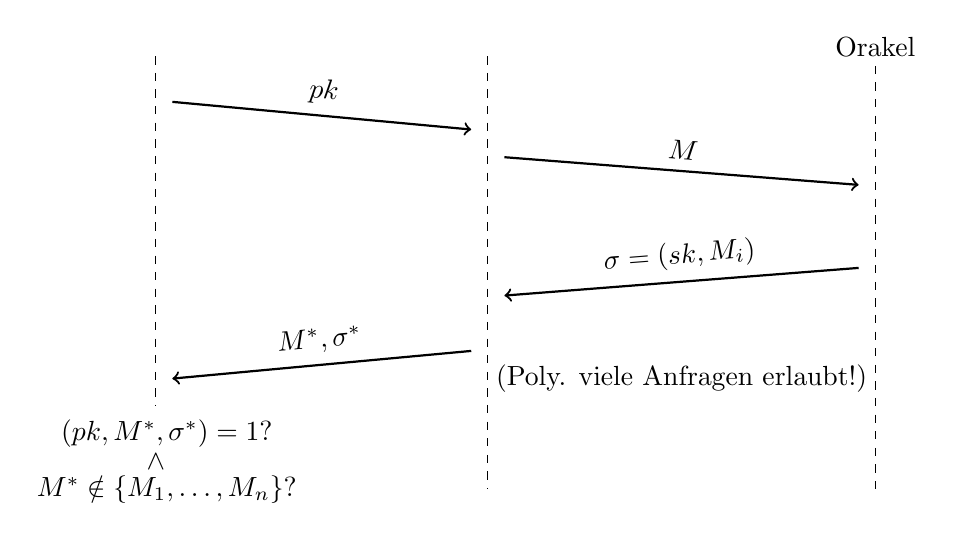
\begin{tikzpicture}[x=2em, y=2em]
      \draw (-6,0) node (C) {$\C$}; 
      \draw (0,0) node (A) {$\A$}; 
      \draw (7,0) node (Ork) {Orakel};
      
      \draw[dashed] (C) -- (-6,-6.5);
      \draw[dashed] (A) -- (0,-8);
      \draw[dashed] (Ork) -- (7,-8);
      
      \textbf{\draw[->, thick] (-5.7,-1) -- (-0.3,-1.5)
        node[sloped,above,pos=0.5] {$pk$}; 
      }
      \textbf{\draw[->, thick] (0.3,-2) -- (6.7,-2.5)
        node[sloped,above,pos=0.5] {$M$};}
      \textbf{\draw[->, thick] (6.7,-4) -- (0.3,-4.5)
        node[sloped,above,pos=0.5] {$\sigma = \sig(sk, M_i)$};}

      \draw (3.5,-6) node (exp) {(Poly. viele Anfragen erlaubt!)};
      
      \textbf{\draw[->, thick] (-0.3, -5.5) -- (-5.7,-6)
        node[sloped,above,pos=0.5] {$M^*, \sigma^*$};}
      
      \draw (-5.8,-7) node (b2) {$\ver(pk, M^*, \sigma^*) = 1$?};
      \draw (-6,-7.5) node (b3) {$\wedge$};
      \draw (-5.8,-8) node (b4) {$M^* \notin \{M_1, \dots, M_n\}$?};
    \end{tikzpicture}
  }
  \caption{Ablauf des EUF-CMA-Experimentes}
  \label{fig:euf-cma}
\end{figure}
\end{center}

\section{Konstruktionen}

\subsection{Hash-then-Sign Paradigma} 
\label{subsec:hash-then-sign}
Viele Signaturverfahren können nur Nachrichten fester Länge
signieren. Für praktische Anwendungen wollen wir aber meist Nachrichten
beliebiger Länge signieren können. Hierzu bieten sich Hash-Funktionen an, die
Nachrichten beliebiger Länge auf einen Bit-String fester Länge abbilden.

Die Idee des \emph{Hash-then-Sign} Paradigmas ist also, anstelle der
vollständigen Nachricht $M~\in~\{0,1\}^*$ den aus ihr berechneten
Hashwert $H(M) \in \{0,1\}^k$ zu signieren. Die
Sicherheit des MACs ist dabei sowohl von der verwendeten Hashfunktion
als auch vom Signaturalgorithmus abhängig.~\\

% Die Idee des \emph{Hash-then-Sign} Paradigmas ist also, nicht die
% vollständige Nachricht $M~\in~\{0,1\}^*$ zu signieren, sondern den aus
% dieser Nachricht berechneten Hashwert $H(M) \in \{0,1\}^k$. Die
% Sicherheit des MACs ist dabei sowohl von der verwendeten Hashfunktion
% als auch vom Signaturalgorithmus abhängig.~\\

\begin{theorem} Sei $(\sig, \ver)$ EUF-CMA-sicher und $H$ eine
  kollisionsresistente Hashfunktion. Dann ist der durch
  \begin{align*} 
    \sig'(K,M) &= \sig(K,H(M))\\ 
    \ver'(K,M,\sigma) &= \ver(K,H(M),\sigma)
  \end{align*} erklärte MAC EUF-CMA-sicher.~\\
\end{theorem}

\begin{beweisidee}
  \label{ch:symauth:eufcma-beweis}
Der  EUF-CMA-Angreifer \A~hat zwei Möglichkeiten. Er kann direkt eine
Signatur $\sigma$ für eine Nachricht \plaint~fälschen. Dies steht aber
im Widerspruch zur vorrausgesetzen EUF-CMA-Sicherheit von $(\sig,
\ver)$, da dann $(H(\plaint), \sigma)$ eine gültige Fälschung für dieses
Schema wäre. Somit kann \A~nur eine im Sicherheitsparameter $k$ vernachlässigbare
Erfolgswahrscheinlichkeit haben. Die zweite Möglichkeit ist, dass er vom
Orakel eine Signatur $\sigma'$ für eine Nachricht $\plaint'$ anfragt und
eine andere Nachricht $\plaint^* \neq \plaint'$ findet, sodass
$\ver'(H^*, \sigma') = \ver(H(\plaint^*), \sigma') = 1$. Aus der
EUF-CMA-Sicherheit von $(\sig,\ver)$ folg aber direkt, dass dafür
$H(\plaint') = H(\plaint^*)$ gelten muss (Ansonsten wäre $(H(\plaint^*,
\sigma'))$ eine gültige Fälschung für $(\sig, \ver)$). D.h. \A~müsste
also eine Kollision berechnen, was er aufgrund der Kollisionsresistenz
der Hashfunktion ebenfalls nur mit in $k$ vernachlässigbarer
Erfolgswahrscheinlichkeit kann. Insgesamt folgt die Behauptung.
\end{beweisidee}

\subsection{Pseudorandomisierte Funktionen}\label{ssec:prf} Wenn man
sich die Berechnung eines MACs als eine einfache Funktion im
mathematischen Sinne vorstellt und damit die Errechnung eines
"`frischen"' MACs zum Finden eines unbekannten Funktionswertes wird,
erkennt man schnell, dass Regelmäßigkeit in einer solchen Funktion zu
Sicherheitslücken führt. Zielführender ist es, die Funktionswerte
möglichst zufällig auf ihre Urbilder zu verteilen.
\begin{definition}[Pseudorandomisierte Funktion (PRF)] Sei  \[\text{\textit{PRF}}\colon\{0,1\}^k \times \{0, 1\}^k \rightarrow
  \{0,1\}^k\] eine über $k \in \mathbbm{N}$ parametrisierte Funktion. $PRF$
  heißt Pseudorandom Function (PRF), falls für jeden PPT-Algorithmus
  $\mathcal{A}$ die Funktion
  \begin{equation*} \text{Adv}_{\text{\textit{PRF}},\mathcal{A}}^{prf}(k)
    := \Pr \lbrack \mathcal{A}^{\text{\textit{PRF}}(K,\cdot)}(1^k) = 1
    \rbrack - \Pr \lbrack \mathcal{A}^{R(\cdot)}(1^k) = 1 \rbrack
  \end{equation*} vernachlässigbar im Sicherheitsparameter $k$ ist, wobei $R: \{0,1\}^k \rightarrow
  \{0,1\}^k$ eine echt zufällige Funktion ist.~\\
\end{definition}

Ein Kandidat für eine solche PRF ist eine Hash-Konstruktion: $PRF(K,X) =
H(K,X)$. Allerdings lässt sich eine solche Konstruktion manchmal, wie
bereits in Abschnitt \ref{ch:hash:merkledamgard} bei Merkle-Damgård
ausgenutzt, nach der Berechnung von $H(K,X)$ auch ohne Zugriff auf das
Geheimnis $K$ noch auf $H(K,X,X')$ erweitern. Das führt dazu, dass die
PRF-Eigenschaft für Eingaben unterschiedlicher Länge nicht mehr
hält. Abbildung \ref{fig:symauth:prf} verdeutlicht das.

\begin{figure}[h]
  \begin{center} \unitlength=1mm \linethickness{0.4pt} \hspace{-3 cm}
    \begin{picture}(70,40)

      \put(10,27){\vector(1,0){15}} \put(17,28){\makebox(0,0)[cb]{IV}}

      \put(30,37){\vector(0,-1){7.5}} \put(33,31){\makebox(0,0)[cb]{$K$}}

      \put(25,24.5){\framebox(10,5){$F$}}

      \put(35,27){\vector(1,0){12}} \put(52,37){\vector(0,-1){7.5}}
      \put(55,31){\makebox(0,0)[cb]{$X$}}

      \put(47,24.5){\framebox(10,5){$F$}}

      \put(57,27){\vector(1,0){8}} \put(75,25){\makebox(0,0)[cb]{$H(K,X)$}}


      \put(0,10){\vector(1,0){15}} \put(7,11){\makebox(0,0)[cb]{IV}}

      \put(20,20){\vector(0,-1){7.5}} \put(23,15){\makebox(0,0)[cb]{$K$}}

      \put(15,7.5){\framebox(10,5){$F$}}

      \put(25,10){\vector(1,0){12}} \put(42,20){\vector(0,-1){7.5}}
      \put(45,15){\makebox(0,0)[cb]{$X$}}

      \put(37,7.5){\framebox(10,5){$F$}}

      \put(47,10){\vector(1,0){12}} \put(64,20){\vector(0,-1){7.5}}
      \put(67,15){\makebox(0,0)[cb]{$X'$}}

      \put(59,7.5){\framebox(10,5){$F$}}

      \put(69,10){\vector(1,0){8}} \put(89,8){\makebox(0,0)[cb]{$H(K,X,X')$}}

      \put(53,4){\makebox(0,0)[cb]{\Large{$\Uparrow$}}}
      \put(53,-2){\makebox(0,0)[cb]{$H(K,X)$ bekannt}}

    \end{picture}
  \end{center}
  \caption{\emph{Merkle-Damgård}-Konstruktion $H_{MD}$. Es ist möglich, an
    einen bereits bekannten Hashwert $H(K,X)$ einen Wert $X'$ anzuhängen und
    trotzdem einen korrekten Hashwert zu erzeugen.}
  \label{fig:symauth:prf}
\end{figure}

Als nächstes wollen wir untersuchen, wie aus einer PRF und einer
kollisionsresistenten Hashfunktion ein EUF-CMA-sicherer MAC Konstruiert
werden kann. 
Dazu sei
\begin{alignat*}{2}
&\sig(K,M): & \sigma \leftarrow \text{\textit{PRF}}(K,H(M)) \\
&\ver(K, M, \sigma):  1 \Leftrightarrow & \sigma \stackrel{?}{=}\text{\textit{PRF}}(K,H(M)).
\end{alignat*}

\begin{theorem} Sei $\text{PRF}\colon\{0,1\}^k \times \{0,1\}^k
  \rightarrow \{0,1\}^k$ eine PRF und $H \colon \{0,1\}^* \rightarrow
  \{0,1\}^k$ eine kollisionsresistente Hashfunktion.  Dann ist der oben
  definierte MAC EUF-CMA-sicher.
\end{theorem} \vspace{10pt}

\begin{beweis}[Entwurf] Sei $\mathcal{A}$ ein erfolgreicher
  EUF-CMA-Angreifer auf ein durch $\sig(K,M) =
  \text{\textit{PRF}}(K,H(M))$ gegebenen MAC. Dann können wir annehmen,
  dass $\mathcal{A}$ eine Fälschung $(M^*,\sigma^*)$ mit einer noch nicht
  signierten Nachricht $M^*$ berechnen kann. Wir können also $\mathcal{A}$
  als \textit{PRF}-Unterscheider auffassen, der mit
  nicht-vernachlässigbarer Wahrscheinlichkeit
  $\text{\textit{PRF}}(K,H(M^*))$ vorhersagt. Eine Vorhersage ist jedoch
  nur dann möglich, wenn \textit{PRF} keinen Zufall ausgibt. Da
  \textit{PRF} jedoch nach Definition nur mit im Sicherheitsparameter $k$ vernachlässigbarer
  Wahrscheinlichkeit von echtem Zufall unterscheidbar ist, kann es einen
  solchen \textit{PRF}-Unterscheider nicht geben.
\end{beweis}

\subsection{HMAC} In Abschnitt \ref{ssec:prf} zu
\hyperref[ssec:prf]{pseudorandomisierten Funktionen}
haben wir gesehen, dass Hashfunktionen, die auf
Merkle-Damgård basieren, beim Einsatz in Signaturverfahren zu Problemen
führen können. Insbesondere sind sie bezüglich der EUF-CMA-Sicherheit
problematisch.  Ein Angreifer, dem $\sigma = H(K,M)$ bekannt ist, erhält
durch Anfügen eines Blockes $X$ problemlos den korrekten Hashwert
$H(K,M,X)$ und somit die Signatur der Nachricht $M,X$.  Dennoch ist es
möglich, EUF-CMA-sichere MACs zu konstruieren, die die Hashfunktionen
verwenden, die auf der Merkle-Damgård-Konstruktion basieren. Eines der verbreitetsten
Verfahren ist der \textit{Keyed-Hash Message Authentication Code}, der
HMAC. Das Signieren einer Nachricht funktioniert dabei wie folgt:
\begin{equation*}
  \sig(K,M) = H(K \oplus \textit{opad}, H(K \oplus
  \textit{ipad}, M))
\end{equation*}
Um eine HMAC $\sigma$ zu prüfen, erstellt der Empfänger selbst eine HMAC
und prüft, ob diese identisch ist zu $\sigma$:
\[\ver (K, M, \sigma) =1 \Leftrightarrow \sigma = H(K \oplus \textit{opad}, H(K \oplus \textit{ipad}, M))\]

Dabei sind \textit{opad}, das \textit{outer padding},
und \textit{ipad}, das \textit{inner padding}, zwei Konstanten der
Blocklänge $m$ der Hashfunktion, die bei jedem Signaturvorgang gleich
bleiben. Üblich\footnote{Sowohl im RFC 2104, sowie in einer
  Veröffentlichung des NIST und in diverser Fachliteratur werden diese
  Werte (als Standard) vorgeschlagen. Siehe: ~\\~\\
  \url{http://tools.ietf.org/html/rfc2104} \\
  \url{http://csrc.nist.gov/publications/fips/fips198-1/FIPS-198-1_final.pdf}}
ist es, $opad = \{0x5C\}^{m/8}$ und $ipad = \{0x36\}^{m/8}$ zu
wählen. 

Auf Grund seiner verschachtelten Struktur ist HMAC gegen den in
Abbildung \ref{fig:symauth:prf} vorgestellten Angriff immun.
Die Nachricht $M$, die es zu Signieren gilt, wird in jeweils zwei
Hash\-vorgängen verarbeitet. Für eine Nachricht $M,X$ ist
\begin{equation*}
 H(K \oplus \textit{opad}, H(K \oplus \textit{ipad}, M), X)
\end{equation*} 
aber offensichtlich keine gültige Signatur. Der
Angreifer müsste einen Nachrichtenblock $X$ bereits im inneren
Hashvorgang unterbringen. Da er dafür allerdings $H$ invertieren, oder
das Geheimnis $K$ kennen müsste, schlägt der Angriff fehl.
\chapter{Asymmetrische Authentifikation von Nachrichten}
\label{cha:asymmauth}

Wie wir bereits bei den Verschlüsselungsverfahren festgestellt haben, weisen symmetrische Verfahren einige Unbequemlichkeiten auf. Allen voran stellt sich das Problem der Schlüsselverteilung, wenn für die Kommunikation zwischen zwei Partnern bei beiden derselbe Schlüssel vorhanden sein muss. Dieses Problem stellt sich natürlich umso mehr, wenn wir über einen nicht vertrauenswürdigen Kanal kommunizieren. Selbst für die Authentifikation unserer Nachrichten, die wir im Zweifelsfall nur betreiben, weil wir dem Kanal nicht vertrauen, müssen wir unter einigem Aufwand Schlüssel mit unseren Kommunikationspartnern festlegen.

Weiterhin ermöglicht symmetrische Authentifikation in keiner sinnvollen Weise, dass wir von uns veröffentlichte Dokumente oder Nachrichten unterschreiben und damit die Urheberschaft für jeden nachprüfbar machen können. Zur Authentifikation des Dokuments sollte schließlich jeder befähigt sein, der sich dafür interessiert. Wenn wir mit symmetrischen Verfahren arbeiten, bedeutet das, dass wir zur Prüfung den Schlüssel herausgeben müssen, mit dem wir das Dokument signiert haben. Das bedeutet aber auch, dass jeder Interessierte nun nicht nur zur Prüfung der bereits bestehenden Signatur in der Lage ist, sondern auch eigene Signaturen erstellen kann. Damit ist die Urheberschaft einer Unterschrift nicht mehr gesichert.

Es bietet sich ein Verfahren an, bei dem die Prüfung einer Signatur nicht mit einem privaten Schlüssel erfolgt. Dieses System kennen wir bereits aus dem Kapitel \ref{ch:asymmenc}. Bei der Verwendung von asymmetrischen Verfahren zur Authentifikation verwenden wir die folgenden Algorithmen:
\begin{itemize}
  \item \textbf{Schlüsselgenerierung:} $(pk, sk) \leftarrow \keygen(1^k)$
    \begin{itemize}
      \item $pk$ : öffentlicher Schlüssel
      \item $sk$ : privater Schlüssel
      \item $k$ : Sicherheitsparameter
    \end{itemize}
  \item \textbf{Signieren:} $\sigma \leftarrow \sig(sk,M)$
  \item \textbf{Verifizieren:} $\ver(pk,M,\sigma) \in \{ 0,1 \}$
\end{itemize}
$\sig$ und $\ver$ müssen korrekt sein, d.h. es muss wie bei MACs gelten:
\begin{equation*}
    \forall (pk,sk) \leftarrow \keygen(1^k), \forall M, \forall \sigma \leftarrow \sig(sk,M) : \ver(pk,M,\sigma) = 1
\end{equation*}
Wir passen außerdem die Definition der EUF-CMA-Sicherheit aus Abschnitt
\ref{ch:symauth:sicherheit} an asymmetrische Verfahren an.

\begin{definition}
Sei \A~ ein PPT-Algorithmus.
\begin{enumerate}
\item \A~erhält Zugriff auf ein Signaturorakel $\sig(sk, \cdot)$ sowie den
  entsprechenden öffentlichen Schlüssel $pk$.
<<<<<<< HEAD
\item \A~darf polynomiell viele Nachrichten $\plaint_i$ an das
  Orakel schicken und erhält $\sigma_i$ mit $\ver(\pkey, \plaint_i, \sigma_i)=1$ als Antwort.
=======
\item \A~darf nun polynomiell viele Nachrichten $\plaint_i$ an das
  Orakel schicken und erhält $\sigma_i \leftarrow \sig(sk, \plaint_i)$ als Antwort.
>>>>>>> upstream/master
\item \A~gibt als (potentielle) Fälschung ein Nachrichten-Signatur-Paar
  $(\plaint^*,\sigma^*)$ aus.
\item \A~gewinnt, wenn $\sigma^*$ eine gültige Signatur für
  $\plaint^*$ ist, d.h. $\ver(\pkey, \plaint^*, \sigma^* = 1)$, und $\plaint^*
  \neq \plaint_i$ für alle $i$ ist, d.h. $\plaint^*$ nicht zu den
  Nachrichten gehört, die sich \A~vom Orakel hat signieren lassen.
\end{enumerate} 

Ein asymmetrisches Signaturverfahren ist EUF-CMA-sicher, wenn jeder
beliebige PPT-Angreifer \A~ das oben genannte Spiel nur mit im
Sicherheitsparameter $k$ vernachlässigbarer Wahrscheinlichkeit gewinnt. 
\end{definition}

Die Definition unterscheidet sich also dadurch, dass
\A~mithilfe des öffentlichen Schlüssels selbst Signaturen verifizieren kann. Anders
als im symmetrischen Fall ist also eine Unterscheidung zwischen zwei
Begriffen mit und ohne Verifikationsorakel nicht nötig. 

\section{RSA}
Wir betrachten zuerst RSA als Kandidaten für ein asymmetrisches
Signaturverfahren. Der Generatoralgorithmus für RSA-Signaturen ist
identisch zu dem für RSA-Verschlüsselung, der in Kapitel
\ref{ch:asymmenc:rsa:vorgehen} besprochen wurde:
\begin{itemize}
 	\item Wähle zwei große Primzahlen $P, Q$ mit $P \neq Q$ und vorgegebener Bitlänge $k$.
 	\item Berechne $N = P \cdot Q$.
 	\item Berechne $\varphi(N) = (P - 1)(Q - 1)$\footnote{$\varphi$
            bezeichnet die Eulersche Phi-Funktion. Sie gibt für jede
            natürliche Zahl n an, wie viele zu n teilerfremde natürliche
            Zahlen es gibt, die nicht größer als n sind: 
            $\varphi(n) := \vert \{a\in\N \, |\, 1 \le a \le n
            \land \operatorname{ggT}(a,n) = 1 \} \vert$. Insbesondere
            ist $\varphi(N)$ die Anzahl multiplikativ invertierbarer
            Elemente im Restklassenring $\mathbb{Z}/N\mathbb{Z}$.
            Sie ist multiplikativ, d.h. es gilt für teilerfremde $n$, $m$:
            $\varphi(m\cdot n) = \varphi(m) \cdot \varphi(n)$. Da eine
            Primzahlen $p$ nur durch 1 und sich selbst teilbar ist, 
            gilt $\varphi(p) = p-1$. Somit gilt für zwei Primzahlen $p$,
            $q$ also $\phi(p \cdot q) = \phi(p) \cdot \phi(q) = (p-1)(q-1)$.}.
 	\item Wähle $e \in \{3, \dotsc, \varphi(N) - 1\}$, wobei
          $\ggT(e, \varphi(N)) = 1$. 
 	\item Berechne mit Hilfe des \hyperref[ssec:eea]{EEA} das zu $e$
          multiplikativ-inverse Element $d$ bezüglich $\varphi(N)$,
          d.h. $d \equiv e^{-1} \pmod{\varphi(N)}$.
        \item $(pk, sk)\leftarrow ((N,e), (N,d))$.
\end{itemize}
Die Signatur- und Verifikationsalgorithmen funktionieren ähnlich wie die
Ver- und Entschlüsselungsalgorithmen aus Kapitel \ref{ch:asymmenc:rsa:vorgehen}\footnote{Oft liest man, dass das Signieren
  von Nachrichten immer dem Verschlüsseln mit dem geheimen Schlüssel
  entspricht. Dies gilt jedoch im Allgemeinen nicht. RSA ist hier eine
  seltene Ausnahme!}:
\begin{alignat*}{3}
& \sig(\skey, \plaint) & = \plaint^d & \mod N\\
& \ver(\pkey, \plaint, \sigma) & = 1 : \Leftrightarrow \plaint = \sigma^e & \mod N 
\end{alignat*}

Das Verfahren hat jedoch einige Nachteile:
\begin{description}
    \item[Signatur \glqq unsinniger\grqq~Nachrichten:] Ein Angreifer
      wählt zunächst ein beliebiges $\sigma \in \mathbbm{Z}$. Dann kann
      er mithilfe des öffentlichen Schlüssels $\pkey$ zu dieser Signatur
      einfach ein $\plaint$ generieren, zu dem die Signatur $\sigma$
      passt: $\plaint := \sigma^e \mod N$.\\ 
    Zwar ist für diesen Angriff im ersten Moment keine sinnvolle Nutzung
    ersichtlich, da der Angreifer keine Kontrolle darüber hat, für
    welche Nachricht er eine Signatur fälscht, die Problematik eines
    Missbrauchs besteht jedoch prinzipiell. Dieser Angriff bricht also
    die für ein Signaturverfahren geforderte EUF-CMA-Sicherheit.
  \item[Homomorphie von RSA:] Angenommen, ein Angreifer ist im Besitz
    zweier Signaturen $\sigma_1$, $\sigma_2$ zu den Nachrichten
    $\plaint_1$, $\plaint_2$. Dann kann er eine gültige Signatur
    $\sigma_3$ für
    eine Nachricht $\plaint_3 = \plaint_1 \cdot \plaint_2 \mod N$
    berechnen mit
    \begin{alignat*}{2}
      \sigma_3 &= \plaint_3^d  & \mod N\\
               &=  (\plaint_1 \cdot \plaint_2)^d & \mod N \\
               &= \plaint_1^d \cdot \plaint_2^d &\mod N\\
               &= \sigma_1 \cdot \sigma_2 &\mod N
    \end{alignat*}
  \end{description}
  Aus der Homomorphie kann man sich einen Angreifer bauen, der das
  EUF-CMA-Sicherheits\-experiment gewinnt: 
  \begin{beispiel}
    Sei \A~ein PPT-Algorithmus und \C~ein Challenger im
    EUF-CMA-Sicherheits\-experiment. Das Experiment läuft wie folgt ab.
    \begin{itemize}
    \item \A~wählt zwei Nachrichten $M_1$, $M_2$ so, dass $ M_1\cdot M_2
      \neq M_i \mod N$ für beide $i$, und sendet diese an \C
    \item \C~erstellt die Signaturen $\sigma_1$, $\sigma_2$ und sendet
      diese an \A
    \item \A~ berechnet $M_3=M_1M_2 \mod N$ und
      $\sigma_3=\sigma_1\sigma_2 \mod N$ und gibt diese aus.
    \end{itemize}
    Damit hat \A~eine Gültige Signatur gefälscht und gewinnt das Experiment.
  \end{beispiel}
Wie bereits bei der RSA-Verschlüsselung in Kapitel \ref{ch:asymmenc:rsa:sicherheit} können wir diese Probleme lösen, indem wir die Nachricht vor der Verarbeitung padden:
\begin{align*}
\sig(\skey,\plaint) &= (\text{pad}(\plaint))^d \mod N\\
\ver(\pkey,\sigma,\plaint) &= 1 :\Leftrightarrow \sigma^e \mod N \text{ ist gültiges Padding für } \plaint
\end{align*}
Das so entstandene Signaturverfahren nennt sich (RSA-)PSS
(\emph{Probabilistic Signature Scheme}) und ist wie RSA-OAEP (als Teil
der \emph{PKCS}) kryptographischer
Standard.\footnote{\url{http://www.emc.com/emc-plus/rsa-labs/standards-initiatives/pkcs-rsa-cryptography-standard.htm}} 
Die \textit{pad}-Funktion wird in Abb. \ref{fig:pss} dargestellt. Sie
erweitert eine Nachticht \plaint~zu einer \textit{encodet Message
  EM}. Das Verifizieren einer so gepaddeten Nachricht wird in
Abb. \ref{fig:pss-vfy} dargestellt. Eine detailierte Erläuterung des
Verfahrens erfolgt hier nicht, kann aber im RFC-Standard 3447
\footnote{\url{https://tools.ietf.org/html/rfc3447}} nachgelesen werden.

\begin{figure}[h]
  \centering
  \begin{subfigure}[b]{.45\textwidth}
    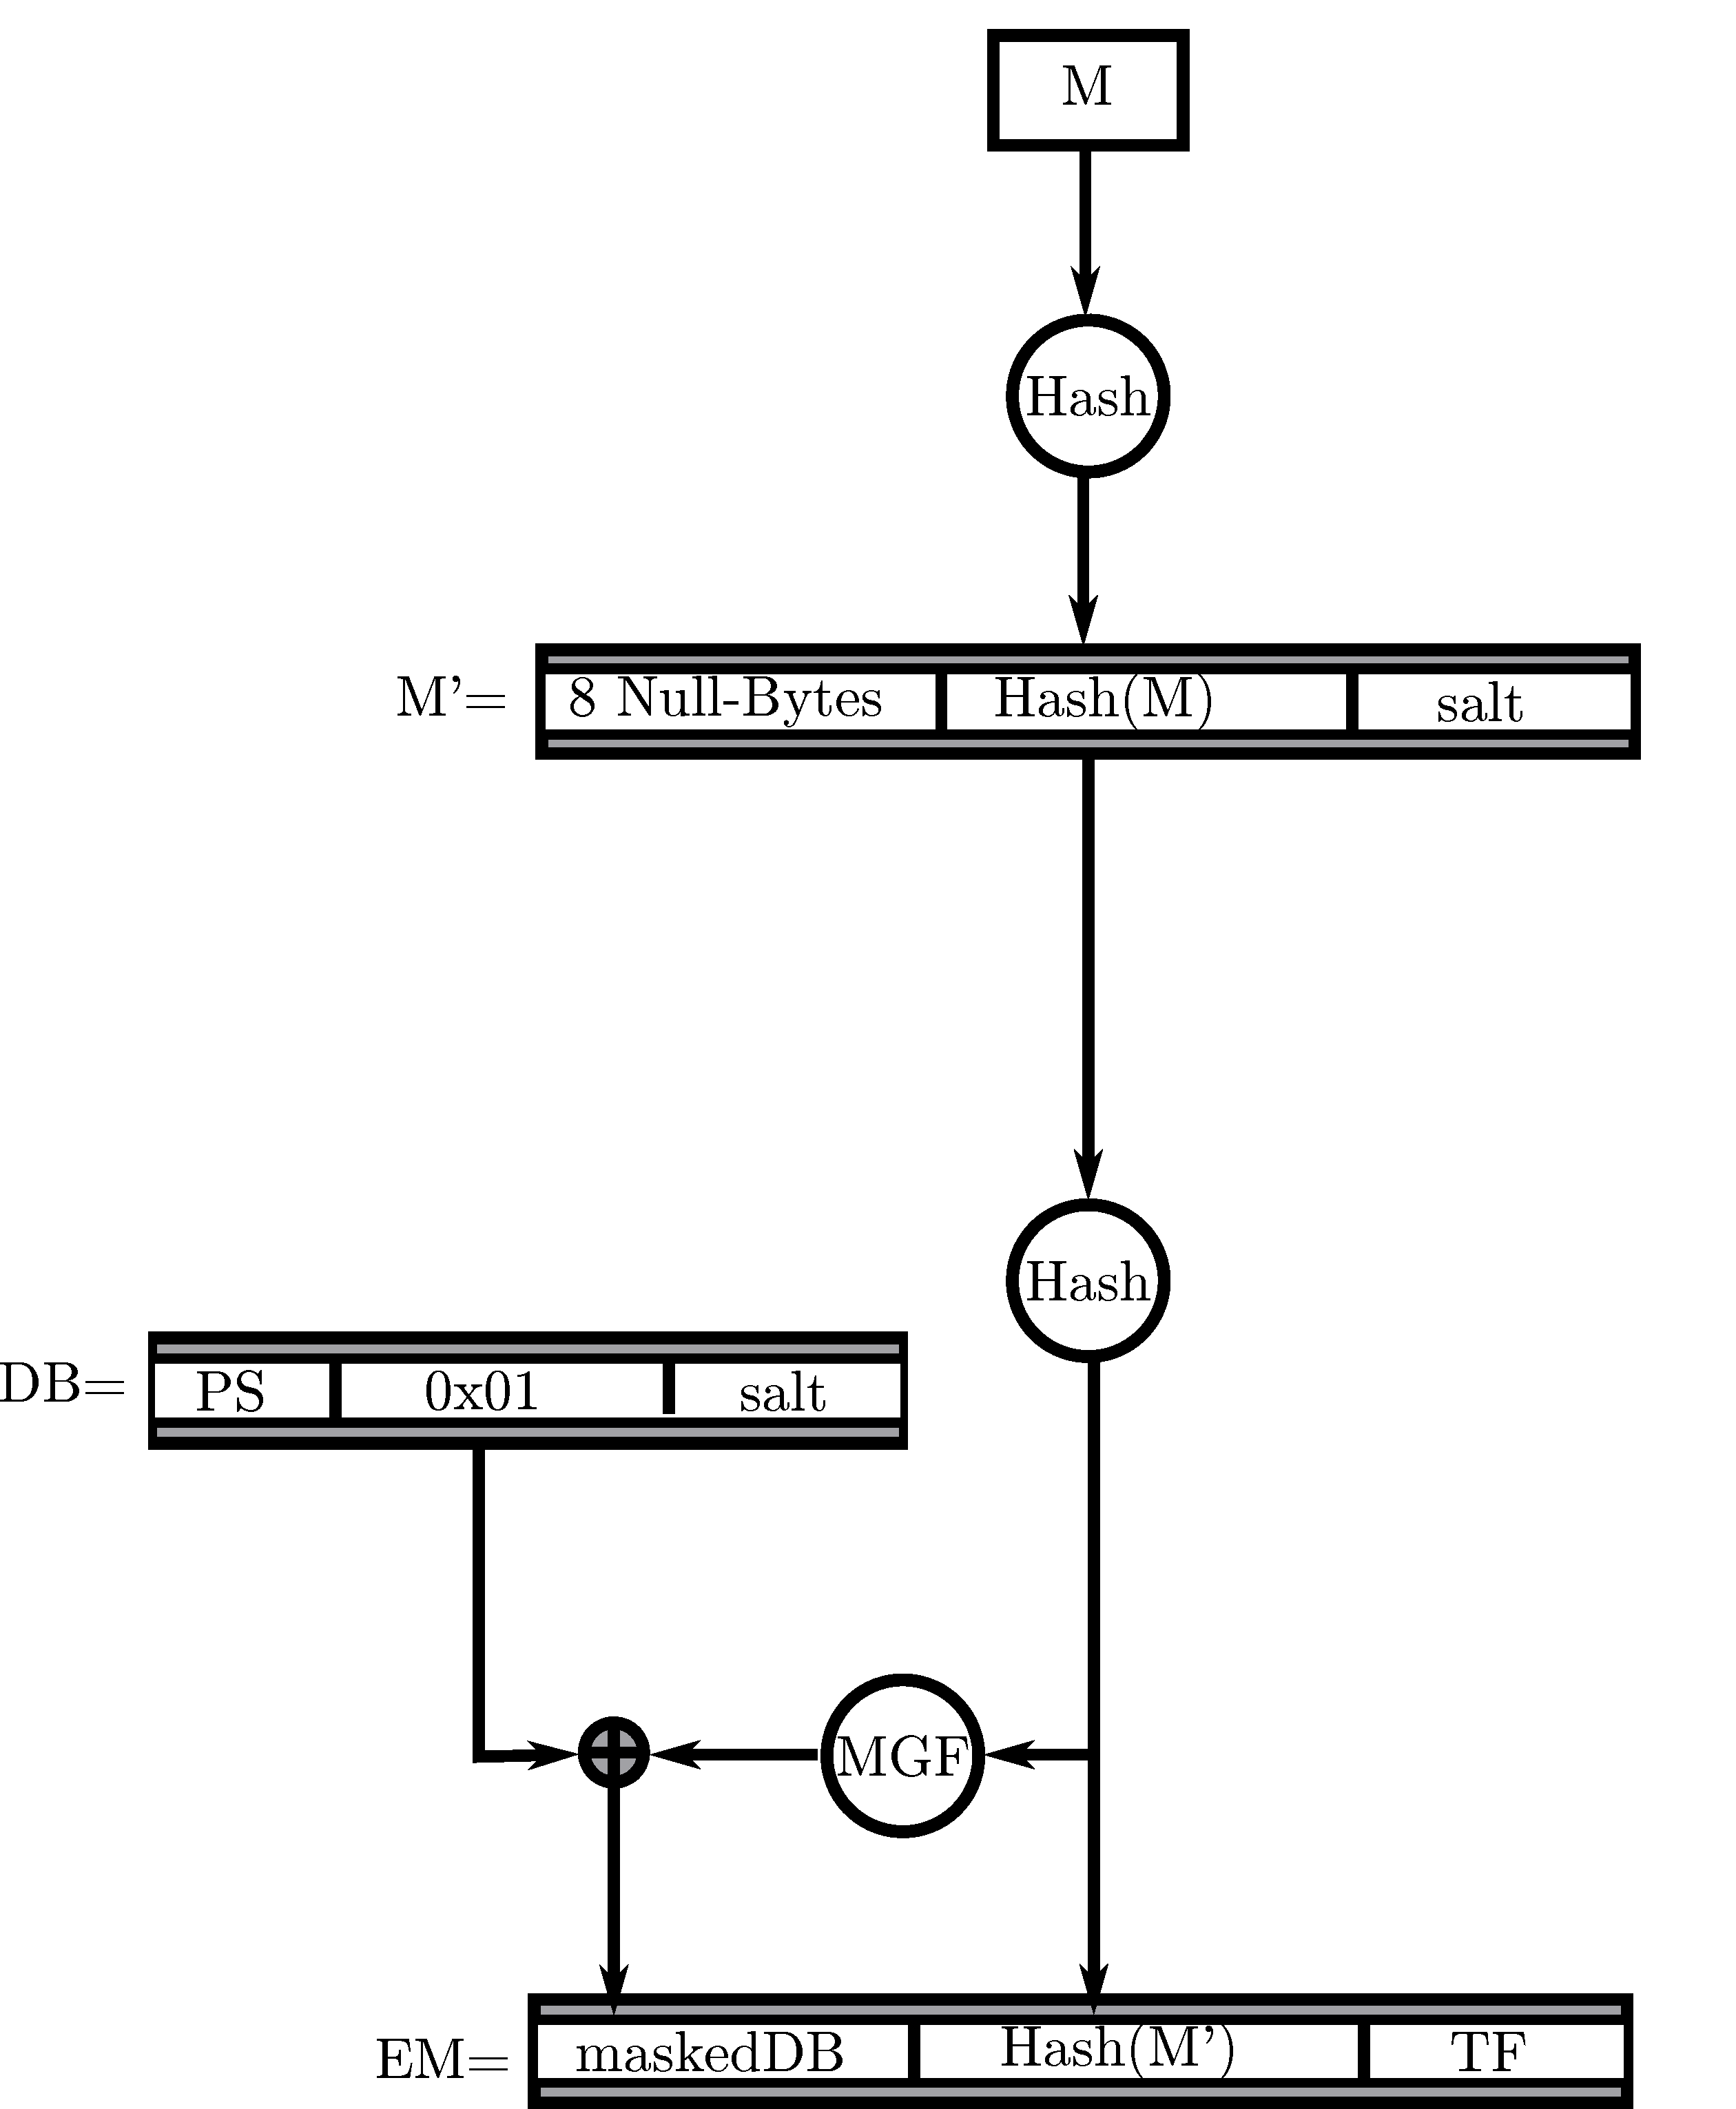
\includegraphics[width=\textwidth]{images/pss.pdf}
    \caption{Padding für RSA-PSS}
    \label{fig:pss}
  \end{subfigure}
  \begin{subfigure}[b]{.45\textwidth}
    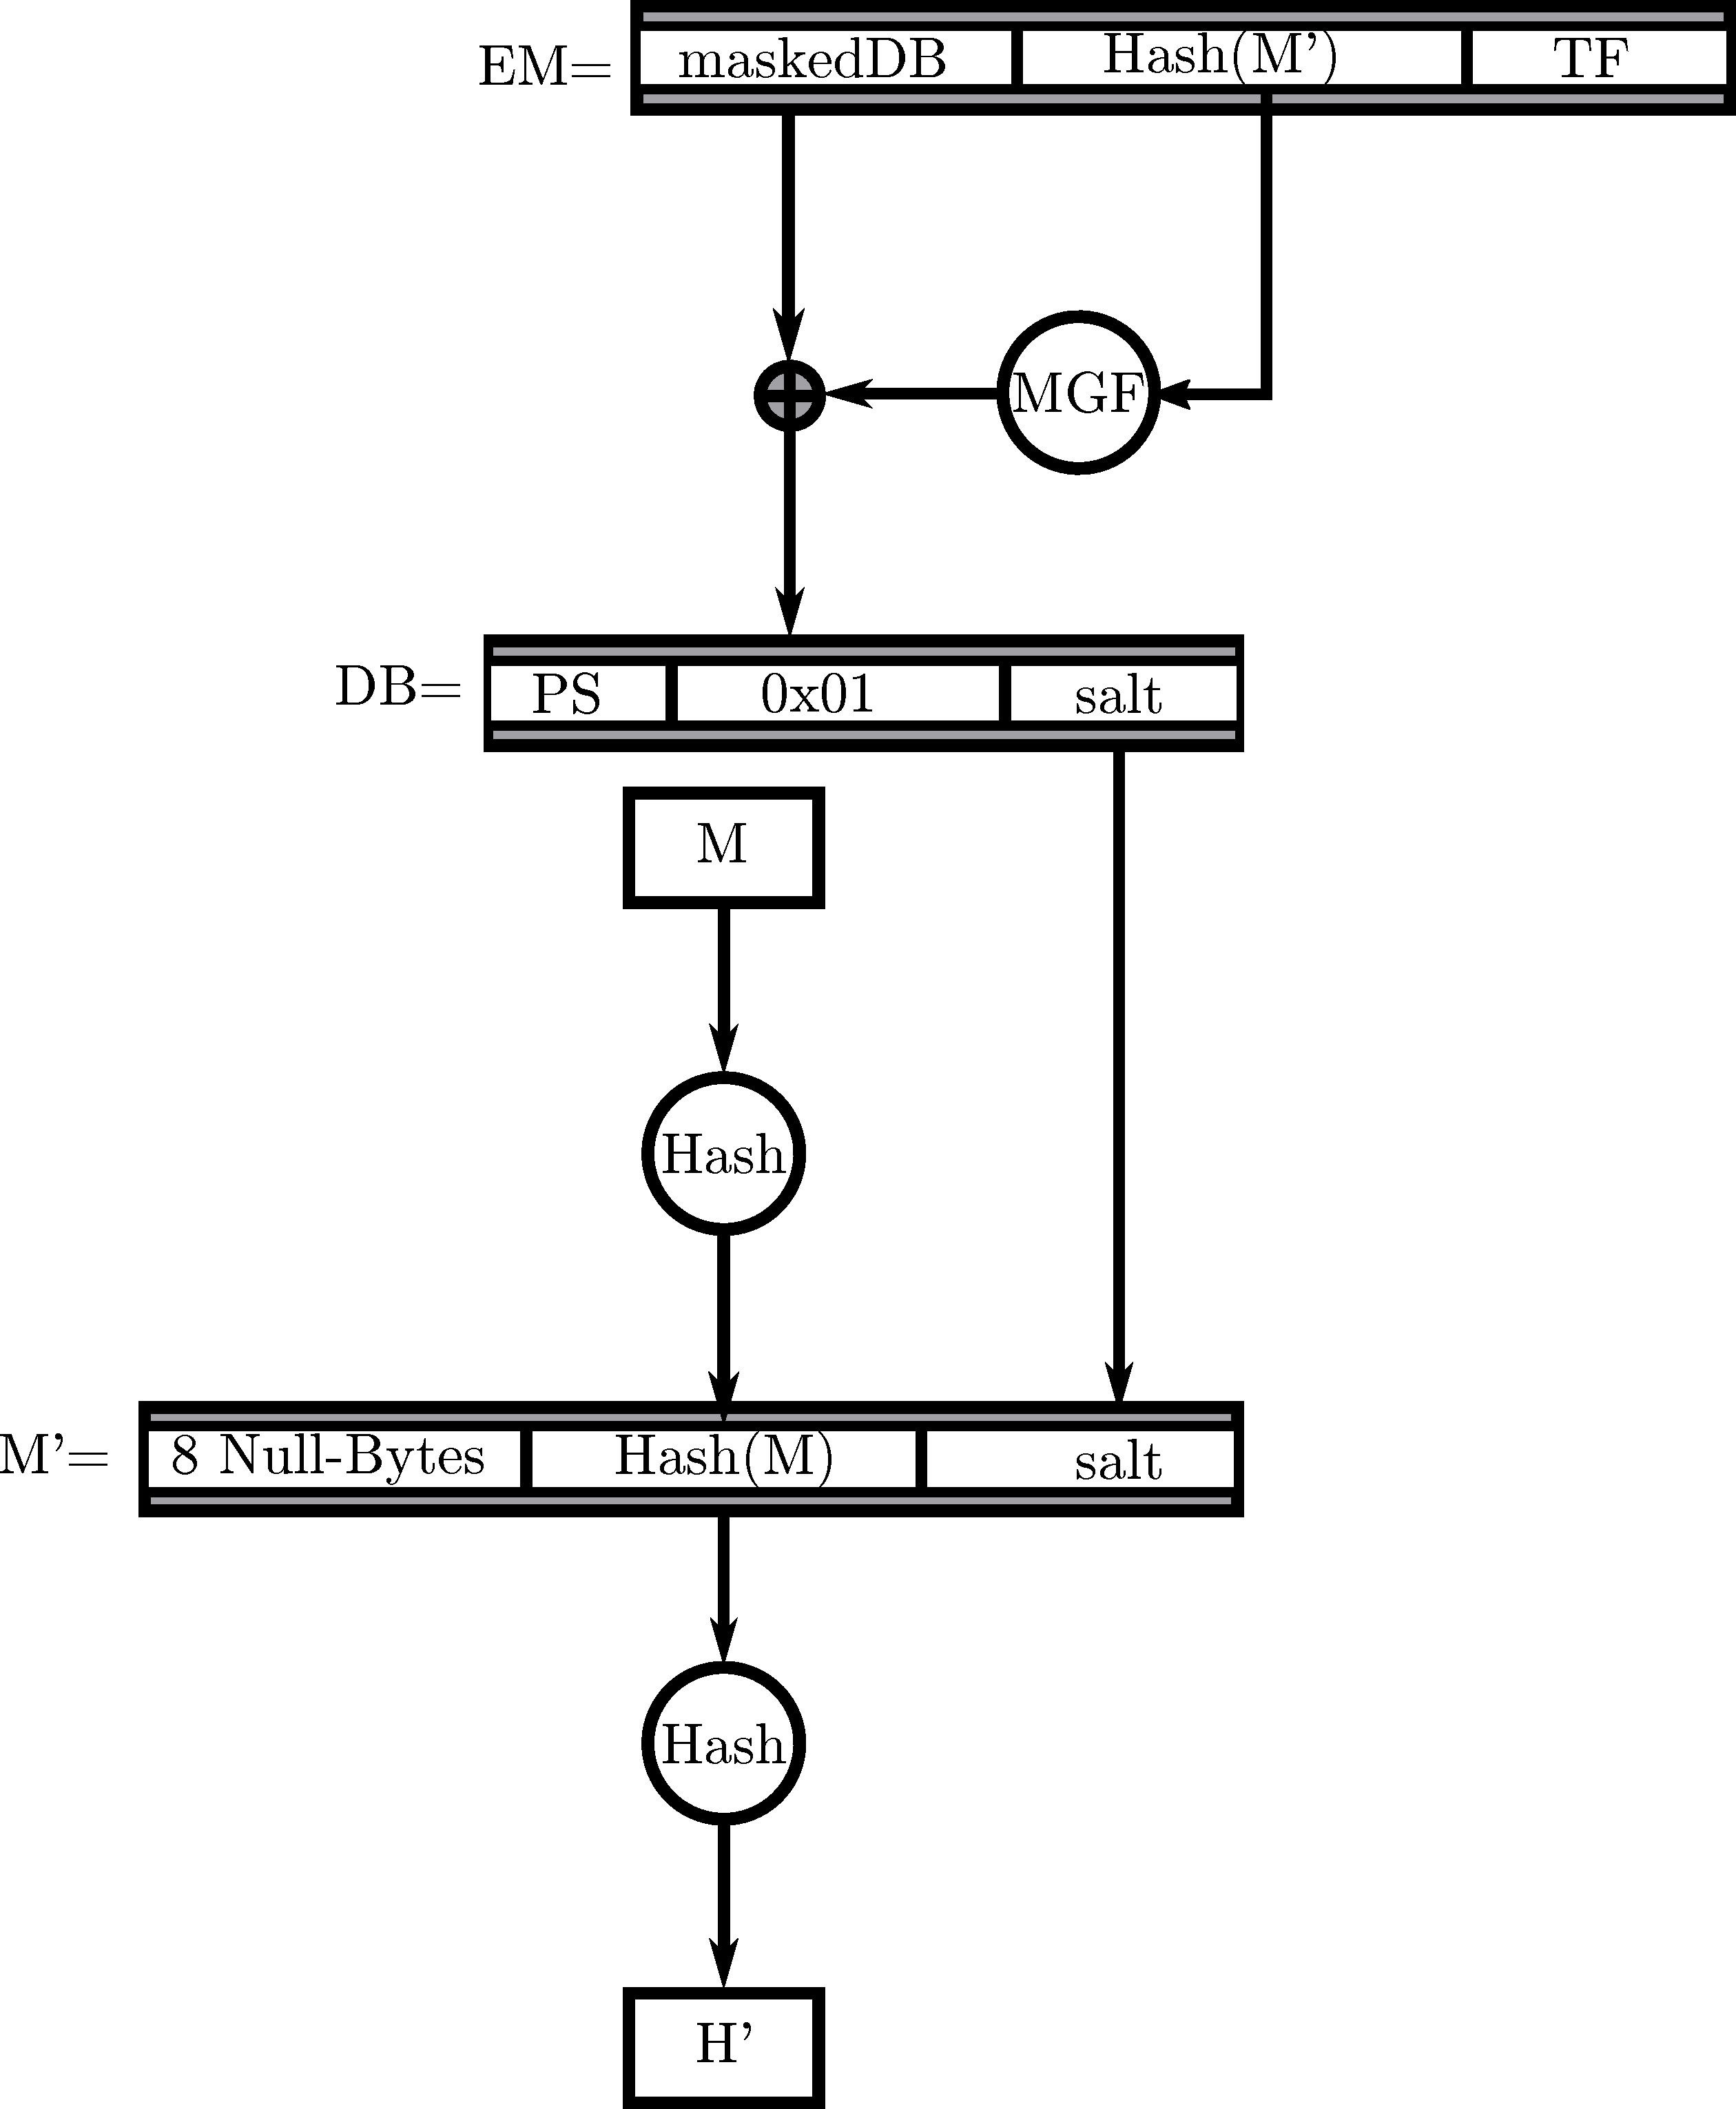
\includegraphics[width=\textwidth]{images/pss-vfy.pdf}
    \caption{Verifikation von gepaddeten Nachrichten}
    \label{fig:pss-vfy}  
  \end{subfigure}
  \caption{Ablauf der Padding-Funktion in RSA-PSS}
\end{figure}


Unter Verwendung idealer Hashfunktionen und mit der Annahme, dass die
RSA-Funktion schwierig zu invertieren ist, ist RSA-PSS heuristisch
EUF-CMA sicher\footnote{D.h. sicher im Random-Oracle-Modell}. Ein Angreifer ist gezwungen, die RSA-Funktion direkt anzugreifen. Der beste bekannte Angriff basiert auf der Faktorisierung von $N$ (unter Verwendung des Zahlkörpersiebs). Die Parameter werden ähnlich wie bei RSA-OAEP gewählt und haben so eine Länge von meistens 2048 Bit. Um eine effiziente Verifikation der Signaturen zu gewährleisten, ist es außerdem ohne Schwierigkeiten möglich, den Parameter $e$ klein zu wählen.


\section{ElGamal}
Analog zum ElGamal-Verschlüsselungssystem aus Kapitel
\ref{ch:asymenc:elgamal} betrachten wir nun ein Signaturverfahren über
der Gruppe $\G = \Z{p}^*$.
\subsection{Erste Idee}
Sei für unseren ersten Versuch der geheime Schlüssel $\skey = (\G, g,
x)$ und der öffentliche Schlüssel $\pkey = (\G, g, h)$ mit $h \equiv g^{x}$. Dann bietet
sich die Verwendung von ElGamal zur Erzeugung einer Signatur auf diese
Art an: 
\begin{align*}
\sig(\skey,M) &= a \text{ mit } a \cdot x = M \mod \left|\G\right|\\
\ver(\pkey,\sigma,M) &= 1 :\Leftrightarrow h^a = g^M
\end{align*}
Allerdings lässt sich diese Konstruktion auf einfache Art brechen, indem
mit $x = M a^{-1} \mod \G$ der geheime Schlüssel berechnet wird. 

\subsection{Schlüssel- und Signaturerzeugung}
Für die Schlüssel gilt weiterhin $\skey = (\G, g,
x)$, $\pkey = (\G, g, h)$ mit $y \equiv g^{x}$. 
Für die Signaturerzeugung wird eine zufällige, in $\Z{p}$ invertierbare
Zahl $e \in \{1, \dots, p - 1\}$ gewählt,
wobei $p=|\G|$. Damit berechnet man 
\begin{align*}
a &:= g^e \in \mathbb{G}\\
b &:= (M - a \cdot x) \cdot e^{-1} \mod p
\end{align*}
$a$ wird je nach Kontext als Gruppenelement oder als Zahl interpretiert, $b$
ist eine Zahl in $\Z{p}$.  
Damit gilt $a \cdot x + e \cdot b = M$. Das Signaturverfahren ist nun
$\sig(\skey,M) = (a, b)$.

Für das Verifikationsverfahren werden nun zwei Gruppenelemente $v_1,
v_2 \in \G$ berechnet mit
\begin{align*}
  v_1 &= h^a \cdot a^b\\
  v_2 &= g^M.
\end{align*}
Das Verifikationsverfahren ist nun
\begin{align*}
\ver(\pkey,\sigma,M) = 1 : & \Leftrightarrow v_1 = v_2 \\
 &\Leftrightarrow h^a \cdot a^b = g^M \\
 &\Leftrightarrow  g^{xa} \cdot g^{be} = g^M
\end{align*}
Doch auch bei dieser Variante gibt es noch einige offene Angriffspunkte:
\begin{description}
	\item[Doppelte Verwendung von $e$:]
	Wird der zufällige Parameter $e$ mehrmals zur Erzeugung von Signaturen verwendet, kann der geheime Schlüssel $x$ aus den beiden Signaturen errechnet werden. Seien die Signaturen $(a = g^e, b, M)$ und $(a' = g^{e} = a, b', M')$. Dann ergibt sich durch Aufaddieren und Umformen
	der Gleichungen
	\begin{align*}
	&a \cdot x + e \cdot b = M\\
	\land \quad &a \cdot x + e \cdot b' = M'\\
	\Rightarrow \quad &e = \frac{M - M'}{b - b'}
	\end{align*}
	Mit bekanntem $e$ kann wiederum auf den geheimen Schlüssel $x$
        geschlossen werden.\footnote{Im Signaturverfahren der
          Spielekonsole \textit{PlayStation 3} (PS 3) wurde dem
          Zufallsparameter $e$ ein immer gleicher Wert zugewiesen,
          wodurch der geheime Schlüssel berechnet werden konnte. Dadurch
          wurde es möglich, unautorisierte Anwendungen, wie
          \textit{gecrackte} Spiele, auf der PS 3 auszuführen. Die
          Erklärung zu diesem erfolgreichen Angriff ist
          \href{https://www.youtube.com/watch?v=4loZGYqaZ7I}{hier} zu
          finden, wobei der Angriff auf das Signaturverfahren ab Minute
          35:30 beschrieben wird.} Bei zufälliger Wahl geschieht es nur
        vernachlässigbar oft, dass zwei Mal dasselbe $e$ ausgewählt wird
        und infolgedessen ausgenutzt werden kann .
	\item[Erzeugung "`unsinniger"' Signaturen:]
	Durch günstige Wahl der Parameter ist es möglich, auch ohne Kenntnis des Schlüssels $x$ gültige Signaturen zu erzeugen. Wähle zunächst $c$
	zufällig. Setze außerdem:
	\begin{align*}
	a &:= g^ch = g^cg^x = g^{c+x}\\
	b &:= -a
	\end{align*}
        Dies impliziert $e=c+x$. 
	Dann ist $(a, b)$ eine gültige Signatur zu $M$ mit
	\begin{align*}
          M &= -ac\\
            &= a \cdot x - a \cdot (c + x)\\
            &= a \cdot x + b \cdot e,\\
	\end{align*}
        denn es gilt 
        \begin{alignat*}{3}
          &&                 & (g^x)^a\cdot a^b       &= &g^M\\
          && \Leftrightarrow & g^{ax} \cdot a^{-a}     &= &g^{-ac}\\
          && \Leftrightarrow & g^{ax} \cdot (g^e)^{-a} &= &g^{-ac}\\
          && \Leftrightarrow & g^{ax-a(c+x)}            &= &g^{-ac}\\
          && \Leftrightarrow & g^{-ac}                 &= &g^{-ac}
        \end{alignat*}
      \end{description}
      \subsection{Beispiel}
      Im Folgenden werden Schlüsselerzeugung, Signieren und Verifizieren beispielhaft
      in der multiplikative Gruppe $\G = \Z{17}^{*}$ mit Ordnung $16$ gezeigt. 
      \subsubsection*{Schlüsselerzeugung}
      Es sind $\skey = (\G, g, x)$ und $\pkey = (\G, g, h)$. Als
      Erzeuger wird $g=3$, als Zufallszahl wird $x=11$
      gewählt. Es sind also $\skey = (\G, 3, 11)$ und $\pkey = (\G, 3,
      3^{11})\equiv (\G, 3, 7)$.
      \subsubsection*{Signieren}
      Alice will eine Nachricht $\plaint = 10$ mit $sk$ signieren. Dazu
      wählt sie einen zufälligen, modulo 16 invertierbaren Exponenten
      $e= 13$ und berechnet mit dem erw. Euklidischen Algorithmus
      $e^{-1}=5$. Dann ist $\sigma =  (a, b)$ mit 
      \begin{align*}
       a &:= g^e &\\
         &= 3^{13} \equiv 12 & \mod 17\\
       b &:= (\plaint-a  \cdot x) \cdot e^{-1} & \mod |\G|\\
          &= (10 - 11 \cdot 12) \cdot 13^{-1} & \mod 16\\
          &\equiv (10 - 11\cdot 12) \cdot 5 \equiv 14 & \mod 16
      \end{align*}
      \subsubsection*{Verifizieren}
      Es ist
      \begin{align*}
        v_1 & = h^a \cdot a^b  & \mod 17 \\
            & = 7^{12} \cdot 12^{14} & \mod 17 \\
            & \equiv 13 \cdot 15 & \mod 17 \\
            & \equiv 8 & \mod 17 \\
        v_2 & = g^M & \mod 17 \\
            &= 3^{10} & \mod 17\\
            &\equiv 8 & \mod 17\\
      \end{align*}
      also gilt $v_1=v_2$ und die Signatur ist gültig.
     

      \section{Hash-Then-Sign-Paradigma}
      Analog zum symmetrischen Fall wollen wir mithilfe des
      Hash-Then-Sign-Paradigmas Nachrichten beliebiger Länge signieren können.
      \begin{theorem}[Hash-Then-Sign-Paradigma]
        Sei $(\keygen, \sig, \ver)$ EUF-CMA-sicher und $H$ eine
        kollisionsresistente Hashfunktion. Dann ist das durch  
        \begin{align*}
          \keygen'(1^k) &= \keygen(1^k)\\
          \sig'(\skey,M) &= \sig(\skey,H(M))\\
          \ver'(\pkey,M,\sigma) &= \ver(\pkey,H(M),\sigma)
        \end{align*}
        definierte Signaturverfahren EUF-CMA-sicher.~\\
      \end{theorem}

      Der Beweis dieses Theorems verläuft analog zu \ref{ch:symauth:eufcma-beweis}.

      Die Verwendung einer kollisionsresistenten Hashfunktion ermöglicht
      eine Abwehr gegen die Erzeugung "`unsinniger"' Signaturen, denn
      die errechneten "`unsinnigen"' Klartexte müssen nun zusätzlich
      denselben Hashwert erzeugen wie die Originalnachricht. 


\section{Digital Signature Algorithm (DSA)}
Aus der Anwendung des Hash-Then-Sign-Paradigmas auf das ElGamal-Signaturverfahren entsteht unter Verwendung einer kollisionsresistenten
Hashfunktion $H$ der \emph{Digital Signature Algorithm} (DSA):
\begin{align*}
a &:= g^e\\
b &:= (H(M) - a \cdot x) \cdot e^{-1} \mod \left|\G\right|
\end{align*}
mit der Signatur $\sigma = (a,b)$.

Der DSA ist nach RSA der zweitwichtigste Signaturalgorithmus und wurde 1994 standardisiert.\footnote{Der aktuelle Standard findet sich auf \url{http://csrc.nist.gov/groups/ST/toolkit/digital_signatures.html}} Für die Bewertung von DSA wirkt sich nachteilig aus, dass für jede neue Signatur eine frische Zufallszahl gewählt werden muss (ein guter Zufallsgenerator wird also
vorausgesetzt) und dass die Verifikation einer DSA-Signatur im Vergleich zu einer RSA-Signatur mit kleinem Modulus deutlich langsamer ist.

Ob DSA EUF-CMA-sicher ist, steht noch nicht eindeutig fest.

\section{Digitale Zertifikate}
Um digital signierte Nachrichten auf ihre Integrität zu prüfen, benötigt
man den öffentlichen Schlüssel. Um sicherzustellen, dass der öffentliche
Schlüssel nicht manipuliert wurde, benutzt man sogenannte PKIs
(\emph{Public Key Infrastructures}). Diese werden oft über digitale
Zertifikate realisiert. Solche Zertifikate werden von einer
sog. \emph{Certificate Authority (CA)} ausgestellt. Überlicherweise
enthalten Zertifikate zumindest
\begin{itemize}
\item den Namen des Ausstellers (\emph{issuer}),
\item den Namen desjenigen, für den das Zertifikat gilt (\emph{subject})
\item einen öffentlichen Schlüssel des \emph{subjects} sowie
\item eine mit dem öffentlichen Schlüssel der CA erstellte Signatur über
  das Zertifikat.
\end{itemize}
Oft werden noch weitere Informationen im Zertifikat gespeichert, wie zum
Beispiel
\begin{itemize}
\item Informationen über das Verfahren, mit dem das Zertifikat generiert wurde,
\item eine Gültigkeitsdauer oder auch
\item Informationen über Rechte des subjects
\end{itemize}

Mithilfe eines solchen Zertifikates kann man sichergehen, dass ein
öffentlicher Schlüssel wirklich zu einer bestimmten Person oder
Institution gehört. Dafür muss man jedoch zum einen der CA trauen, zum
anderen braucht man den öffentlichen Schlüssel der CA. 

Das Vertrauen in die CA ist in vielen Anwendungen ein großes Problem. Im
Webbrowser Firefox werden beispielsweise 194 Zertifizierungsstellen
berechtigt, Zertifikate auszustellen\footnote{Stand 28.06.2016. Quelle:
  \url{https://hg.mozilla.org/mozilla-central/raw-file/tip/security/nss/lib/ckfw/builtins/certdata.txt}}. Alle
Zertifiezierungsstellen müssen vertrauenswürdig sein, da sonst
kompromitierte Zertifikate in Umlauf kommen können.

\subsection{X.509}
Der am weitesten verbreitete Standard für Zertifikate ist X.509. Ein
solches Zertifikat findet sich in Abb. \ref{fig:x509}
\begin{figure}
\begin{lstlisting}
Certificate:
    Data:
        Version: 3 (0x2)
        Serial Number: 1 (0x1)
        Signature Algorithm: md5WithRSAEncryption
        Issuer: C=AT, ST=Steiermark, L=Graz, O=TrustMe Ltd,
                OU=Certificate Authority, CN=CA/Email=ca@trustme.dom 
        Validity
            Not Before: Oct 29 17:39:10 2000 GMT
            Not After : Oct 29 17:39:10 2001 GMT
        Subject: C=AT, ST=Vienna, L=Vienna, O=Home, OU=Web Lab,
                 CN=anywhere.com/Email=xyz@anywhere.com 
        Subject Public Key Info:
            Public Key Algorithm: rsaEncryption
            RSA Public Key: (1024 bit)
                Modulus (1024 bit):
                    00:c4:40:4c:6e:14:1b:61:36:84:24:b2:61:c0:b5:
                    d7:e4:7a:a5:4b:94:ef:d9:5e:43:7f:c1:64:80:fd:
                    9f:50:41:6b:70:73:80:48:90:f3:58:bf:f0:4c:b9:
                    90:32:81:59:18:16:3f:19:f4:5f:11:68:36:85:f6:
                    1c:a9:af:fa:a9:a8:7b:44:85:79:b5:f1:20:d3:25:
                    7d:1c:de:68:15:0c:b6:bc:59:46:0a:d8:99:4e:07:
                    50:0a:5d:83:61:d4:db:c9:7d:c3:2e:eb:0a:8f:62:
                    8f:7e:00:e1:37:67:3f:36:d5:04:38:44:44:77:e9:
                    f0:b4:95:f5:f9:34:9f:f8:43
                Exponent: 65537 (0x10001)
        X509v3 extensions:
            X509v3 Subject Alternative Name:
                email:xyz@anywhere.com
            Netscape Comment:
                mod_ssl generated test server certificate
            Netscape Cert Type:
                SSL Server
    Signature Algorithm: md5WithRSAEncryption
        12:ed:f7:b3:5e:a0:93:3f:a0:1d:60:cb:47:19:7d:15:59:9b:
        3b:2c:a8:a3:6a:03:43:d0:85:d3:86:86:2f:e3:aa:79:39:e7:
        82:20:ed:f4:11:85:a3:41:5e:5c:8d:36:a2:71:b6:6a:08:f9:
        cc:1e:da:c4:78:05:75:8f:9b:10:f0:15:f0:9e:67:a0:4e:a1:
        4d:3f:16:4c:9b:19:56:6a:f2:af:89:54:52:4a:06:34:42:0d:
        d5:40:25:6b:b0:c0:a2:03:18:cd:d1:07:20:b6:e5:c5:1e:21:
        44:e7:c5:09:d2:d5:94:9d:6c:13:07:2f:3b:7c:4c:64:90:bf:
        ff:8e
\end{lstlisting}
\caption{Beispiel für ein X.509-Zertifikat}
\label{fig:x509}
\end{figure}

Das Zertifikat ist in zwei Blöcke  unterteilt. Der erste (\texttt{Data})
enthält die Daten, über die das Zertifikate Aussagen macht. Der zweite
Teil (\texttt{Signature Algorithm}) gibt das Verfahren an, mit dem die
Signatur erstellt wurde. Darauf folgt die Signatur.

Der \texttt{Data}-Abschnitt enthält verschiedene Daten:
\begin{itemize}
\item \texttt{Version}: die Version von X509, die verwendet wurde
\item \texttt{Serial Number}: Eine Seriennummer, die für jede CA
  eindeutig sein muss
\item \texttt{Signature Algorithm}: Das Verfahren, mit dem die Signatur
  erstellt wurde.
\item \texttt{Issuer}: Informationen über die CA
\item \texttt{Validity}: Daten, ab wann und bis wann das Zertifikat
  gültig ist
\item \texttt{Subject}: Informationen über die Institution, deren
  öffentlicher Schlüssel zertifiziert wird.
\item \texttt{Subject Public Key Info}: Infomationen über den
  öffentlichen Schlüssel sowie den Schlüssel selbst.
\item \texttt{X509v3 extensions}: Hier kann X509 mit Erweiterungen
  versehen werden, um an besondere Anforderungen angepasst zu werden.
\end{itemize} 
\chapter{Schlüsselaustauschprotokolle}
\label{cha:keyexchange}

In diesem Kapitel widmen wir uns der offenen Frage nach dem Schlüsselaustauschproblem, das insbesondere bei der Besprechung von symmetrischen Verschlüsselungs-
und Signaturverfahren einige Male aufgekommen ist. Zwei Kommunikationspartner Alice und Bob können ohne vorherigen Schlüsselaustausch keine sichere Verbindung
einrichten. Allerdings werden sie nicht jedes Mal die Möglichkeit haben, sich vor ihrer eigentlichen Kommunikation privat zu treffen, um einen gemeinsamen
Sitzungsschlüssel auszuhandeln. Vielleicht kennen sie einander nicht einmal persönlich, auf jeden Fall aber wäre ein solches Vorgehen sichtlich nicht
praktikabel.

Alice und Bob müssen also die unsichere Leitung zum Schlüsselaustausch verwenden. Den Schlüssel im Klartext darüber zu senden, würde einen Mithörer
trivial in die Situation bringen, auch den verschlüsselten Teil der darauf folgenden Kommunikation mitzulesen. Der neue Sitzungsschlüssel
$\key$ von Alice und Bob muss also bereits so über die Leitung gesendet werden, dass ein Lauscher nicht in der Lage ist, den Schlüssel zu rekonstruieren. Dabei
sind folgende grundlegende Szenarien denkbar:
\begin{itemize}
  \item Alice und Bob besitzen bereits einen alten Schlüssel $\key'$ aus einem früheren Austausch und möchten ein frisches $\key$ erzeugen
  \item es existierte eine Secret-Key-Infrastruktur mit einer Schlüsselzentrale (Alice besitzt einen Schlüssel $\key_A$, Bob $\key_B$ und
  die Schlüsselzentrale beide)
  \item es existiert eine Public-Key-Infrastruktur ($\pkey_A, \pkey_B$ sind öffentlich, Alice besitzt $\skey_A$, Bob besitzt $\skey_B$)
  \item Alice und Bob besitzen ein gemeinsames Passwort
  \item Alice und Bob besitzen keine gemeinsamen Informationen
\end{itemize}


\section{Symmetrische Verfahren}
Als Grundszenario für symmetrische Verfahren wird hier ein System mit einer Secret-Key-Infrastruktur gewählt. Das bedeutet, dass jeder
Teilnehmer einen geheimen, symmetrischen Schlüssel mit der Schlüsselzentrale hat. Jeder Verbindungsaufbau mit einem
anderen Teilnehmer beginnt deshalb mit einer Anfrage an die Zentrale. Da die Zentrale die Anlaufstelle für viele Teilnehmer ist, sollte die Kommunikation mit
dieser Stelle möglichst minimiert werden, was die vollständige Kommunikation der beiden Teilnehmer Alice und Bob über die Zentrale ausschließt. Gleichzeitig sind jedoch die Leitungen
nicht vertrauenswürdig, sodass die Kommunikation über große Strecken verschlüsselt stattfinden sollte.

\subsection{Kerberos}
Eine Lösung für dieses Szenario bietet das Protokoll \emph{Kerberos} an, das in Abbildung \ref{fig:keyex:kerberos} in seiner ursprünglichen
Form dargestellt ist. Alice sendet dabei der Schlüsselzentrale eine Anfrage, die ihren Namen und den ihres gewünschten Gesprächspartners
erhält und bekommt dafür von der Zentrale zwei Pakete zurück, von denen eines mit ihrem und eins mit Bobs Schlüssel verschlüsselt ist. Beide
Pakete erhalten den gemeinsamen Sitzungsschlüssel $K$, sowie die Lebensdauer $L$ des Schlüssels und einen Zeitstempel $T_{KC}$ der Schlüsselzentrale, der
Replay-Attacken erschwert.
Alice entpackt das an sie adressierte Paket, erhält den Sitzungsschlüssel und leitet nach Prüfung von $L$ und $T$ das für Bob vorbereitete Paket weiter. Sie
fügt außerdem eine mit $K$ verschlüsselte Nachricht bei, in der sie ihre Identität und einen von ihr erstellten Zeitstempel $T_A$ einfügt.

Bob überprüft seinerseits den Zeitstempel der Zentrale und die Lebensdauer des Sitzungsschlüssels und dechiffriert dann Alices Nachricht mit dem neuen
Sitzungsschlüssel. Er kann nun sowohl den Zeitstempel überprüfen als auch, ob die Anfrage an die Schlüsselzentrale vom selben Teilnehmer stammt wie die mit dem
Sitzungsschlüssel chiffrierte Nachricht. Außerdem kann er bei erfolgreicher Entschlüsselung sicher sein, dass Alice $K$ besitzt. Er sendet nun seinerseits eine
mit $K$ verschlüsselte Nachricht an Alice, mit der er nachweist, dass er den Sitzungsschlüssel besitzt. Mit der Erhöhung des Zeitstempels kann er außerdem
beweisen, dass er die korrekte Nachricht erhalten und dechiffriert hat.

\begin{figure}[h]
\begin{center}
\unitlength=1mm
\linethickness{0.4pt}
\hspace{-3 cm}
	\begin{picture}(120,60)(-10,0)
		\put(0,53){\makebox(0,0)[cb]{\texttt{Alice}$_{\key_A}$}}
		\put(100,53){\makebox(0,0)[cb]{\texttt{Schlüsselzentrale (KC)$_{\key_A, \key_B}$}}}
		\put(120,28){\makebox(0,0)[cb]{\texttt{Bob$_{\key_B}$}}}
	
		\put(0,2){\line(0,1){50}}
		\put(100,30){\line(0,1){22}}
		\put(120,2){\line(0,1){25}}
		
		\put(50,46){\makebox(0,0)[cb]{(Alice, Bob)}}
		\put(0,45){\vector(1,0){100}}
	
		\put(50,36){\makebox(0,0)[cb]{$\enc(\key_A,(T_{KC}, L, \key, \text{Bob}))$, $\enc(\key_B, (T_{KC}, L, \key, \text{Alice}))$}}
		\put(100,35){\vector(-1,0){100}}
		
		\put(60,20){\makebox(0,0)[cb]{$\enc(\key, (\text{Alice}, T_A))$, $\enc(\key_B, (T_{KC}, L, \key, \text{Alice}))$}}
		\put(0,19){\vector(1,0){120}}
		
		\put(60,10){\makebox(0,0)[cb]{$\enc(K, T_A+1)$}}
		\put(120,9){\vector(-1,0){120}}
	
	\end{picture}
\end{center}
\caption{Ursprüngliches Schlüsselaustauschprotokoll Kerberos. $T_X$ bezeichnet einen von $X$ ausgestellten Zeitstempel, $\key$ den
erzeugten Sitzungsschlüssel für Alice und Bob und $L$ seine Lebensdauer.}
\label{fig:keyex:kerberos}
\end{figure}

Die verschachtelte Konstruktion von Kerberos verhindert Man-in-the-Middle-Angriffe. Die Kodierung der Absender- und Empfängernamen durch die
Schlüsselzentrale ermöglicht eine Authentifizierung der Kommunikationsteilnehmer und der Einsatz von Zeitstempeln sowie die Zuordnung
einer Lebensdauer zu einem Schlüssel erschwert zudem Replay-Attacken.
Nichtsdestotrotz ist für das Protokoll ein aktiv sicheres Verschlüsselungsverfahren nötig. Über die Sicherheit von Kerberos lässt sich also
formal keine Aussage treffen.

\section{Asymmetrische Verfahren}
Als Grundlage für die folgenden Schlüsselaustauschprotokolle nutzen wir eine Public-Key Infrastruktur. Die Schlüssel werden wie in Kapitel
\ref{ch:asymmenc} von den Teilnehmern selbst erzeugt. Jeder hält also seinen privaten Schlüssel geheim. Die öffentlichen Schlüssel
hinterliegen an einem allgemein zugänglichen Ort und sind von einer vertrauenswürdigen Stelle zertifiziert.

\subsection{Public-Key Transport}
Das einfachste Verfahren, das sich zum Schlüsselaustausch in Public-Key-Infrastruktur anbietet, nennt sich \emph{Public-Key Transport}. Alice erzeugt einen
Sitzungsschlüssel, den sie für die Kommunikation mit Bob verwenden will. Die bereits bestehende Infrastruktur wird nun dafür
genutzt, den Sitzungsschlüssel mit Bobs öffentlichem Schlüssel zu chiffrieren und an Bob zu senden (siehe Abb.
\ref{fig:keyex:publickeytransport}).

\begin{figure}[h]
\begin{center}
\unitlength=1mm
\linethickness{0.4pt}
\hspace{-3 cm}
\begin{picture}(30,10)
\put(0,2){\makebox(0,0)[cb]{$\text{Alice}_{\skey_A}$}}
\put(10,3){\vector(1,0){40}}
\put(30,4){\makebox(0,0)[cb]{$C := \enc(\pkey_B, \key)$}}
\put(55,0.5){\makebox(10,5){$\text{Bob}_{\skey_B}$}}
\end{picture}
\end{center}
\caption{Während des Protokolls Public-Key Transport wählt Alice einen Sitzungsschlüssel $\key$ und sendet ihn unter Ausnutzung der zur
Verfügung stehenden Public-Key-Infrastruktur an Bob.}
\label{fig:keyex:publickeytransport}
\end{figure}

Vorausgesetzt, das verwendete Public-Key-Verfahren ist IND-CPA-sicher, kann der Angreifer $\ciphert$ nicht vom Zufall unterscheiden oder den darin
enthaltenen Sitzungsschlüssel extrahieren. Public-Key Transport ermöglicht also passive Sicherheit gegenüber einem Angreifer, der $\ciphert$ auf der Leitung
mithören kann.

Allerdings bietet das Verfahren in dieser Form keine Möglichkeit zur Authentifizierung der Kommunikationsteilnehmer an. Das lässt sich durch
das Hinzufügen von Signaturen wie in Abbildung \ref{fig:keyex:publickeytransportauth} lösen. Trotzdem ist es dann noch immer möglich, einen
Replay-Angriff durchzuführen und $\ciphert$ zu einem späteren Zeitpunkt noch einmal zu senden, ohne dass Bob der Fehler sofort auffällt.

\begin{figure}[h]
\begin{center}
\unitlength=1mm
\linethickness{0.4pt}
\hspace{-3 cm}
\begin{picture}(120,10)(-15,0)
\put(0,0){\makebox(0,0)[cb]{$\text{Alice}_{\skey_{\text{PKE,}A}, \skey_{\sig, A}}$}}
\put(16,3){\vector(1,0){80}}
\put(55,4){\makebox(0,0)[cb]{$(C := \enc(\pkey_{\text{PKE,}B}, \key),$}}
\put(55,-2){\makebox(0,0)[cb]{$\sigma := \sig(\skey_{\sig, A}, C))$}}
\put(110,0){\makebox(10,5){$\text{Bob}_{\skey_{\text{PKE,}B}, \skey_{\sig, B}}$}}
\end{picture}
\end{center}
\caption{Digitale Signaturen ermöglichen den Ausbau des Protokolls Public-Key Transport auf die Authentifikation der Teilnehmer.}
\label{fig:keyex:publickeytransportauth}
\end{figure}

\subsection{Diffie-Hellman-Schlüsselaustausch}
Der Diffie-Hellman-Schlüsselaustausch (1976) hat auf den ersten Blick Ähnlichkeit mit dem asymmetrischen Verschlüsselungsverfahren von
ElGamal (1985). Auch hier benötigen wir eine ausreichend große, zyklische Gruppe $\G = \langle g \rangle$ mit Ordnung $q$. Alice und Bob wählen sich
jeweils eine Zufallszahl $x, y \in \mathbbm{Z}_q$ und schicken $g^x$ bzw. $g^y$ an den jeweils anderen. Jeder von beiden ist nun in der Lage, $g^{xy}$
zu berechnen.

Das Berechnen des gemeinsamen Geheimnisses $g^{xy}$ als Außenstehender bezeichnet man als \emph{computational Diffie-Hellman}-Problem (CDH-Problem).
Dabei hat ein Angreifer Zugriff auf das Generatorelement und die beiden Zahlen $g^{x}$, $g^{y}$. Die Sicherheit des Verfahrens beruht auf der sogenannten
\emph{computational Diffie-Hellman}-Annahme (CDH-Annahme), die besagt, dass das Lösen des CDH-Problems in manchen zyklischen Gruppen schwer ist.
Aktive Angriffe, wie Replay- oder Man-in-the-Middle-Attacken, sind damit allerdings nicht ausgeschlossen.

\begin{figure}[h]
	\begin{center}
		\unitlength=1mm
		\linethickness{0.4pt}
		\hspace{-3 cm}
		\begin{picture}(80,50)(-10,0)
			\put(10,42){\makebox(0,0)[cb]{\texttt{Alice}$_x$}}
			\put(10,10){\line(0,1){30}}
	
			\put(70,42){\makebox(0,0)[cb]{\texttt{Bob}$_y$}}
			\put(70,10){\line(0,1){30}}
		
			\put(40,31){\makebox(0,0)[cb]{$g^x$}}
			\put(10,30){\vector(1,0){60}}
		
			\put(40,21){\makebox(0,0)[cb]{$g^y$}}
			\put(70,20){\vector(-1,0){60}}
	
			\put(40,0){\makebox(0,0)[cb]{$(g^y)^x \qquad = \qquad g^{xy} \qquad = \qquad (g^x)^y$}}
		\end{picture}
	\end{center}
	\caption{Diffie-Hellman-Schlüsselaustausch}
	\label{fig:keyex:dh}
\end{figure}

\section{Transport Layer Security (TLS)}
\label{sec:keyexchange:tls}
Dieses Kapitel befasst sich mit einem Protokoll zum Schlüsselaustausch zweier einander unbekannter Kommunikationspartner.
Die klassische Motivation hierfür sind Einkäufe mit der Kreditkarte. Dabei ist es nicht ausschließlich Alices Sorge, dass die Daten unterwegs
abgefangen und für andere Käufe verwendet werden könnten. Ein Angreifer könnte außerdem die Kaufsumme ihres Auftrags
manipulieren oder sich für den Server ausgeben, mit dem Alice kommunizieren möchte und dem sie ihre Kreditkartendaten überträgt.

Dieses Problem, das gleichzeitig den Schlüsselaustausch, wie auch die Authentifikation der Kommunikationspartner umfasst, beschränkt sich allerdings nicht auf
den Interneteinkauf über \emph{http} sondern auch auf andere Anwendungsprotokolle wie \emph{ftp} zur Übertragung von Dateien und \emph{imap} und \emph{smtp},
denen Alice ihre E-Mail-Passwörter anvertraut.

Kurz gefasst benötigt Alice also ein Protokoll, das die Integrität der übertragenen Daten sowie die Authentifikation des Senders bzw. Empfängers implementiert
und einen sicheren Schlüsselaustausch zur Verfügung stellt. Gleichzeitig sollte es möglichst viele Anwendungsprotokolle abdecken, damit nicht jedes einzeln
abgesichert werden muss.

Zu diesem Zweck wurde SSL (\emph{Secure Socket Layer}) entwickelt und in 1999 mit einigen Änderungen als TLS (\emph{Transport Layer Security}) standardisiert.
TLS ist ein hybrides Protokoll zum Aufbau und Betrieb sicherer Kanäle über ein eigentlich unsicheres Medium, einschließlich eines Schlüsselaustauschs.
Dafür wird erst ein authentifizierter asymmetrischer Schlüsselaustausch durchgeführt und danach mit diesem ausgehandelten Schlüssel symmetrisch
verschlüsselt kommuniziert. Es ist sogar möglich, einen Schlüssel neu auszuhandeln, falls der Verdacht besteht, dass er kompromittiert
ist. Außerdem bietet TLS eine ganze Reihe an Schlüsselaustausch- und Verschlüsselungsalgorithmen an, auf die die beiden Parteien sich
einigen können.

% Transportschicht sollte kurz erklärt werden
Dadurch, dass TLS auf der Transportschicht\footnote{Die Transportschicht ist die 4. Schicht des OSI-Modells, eine in Schichten gegliederte Architektur für Netzwerkprotokolle. Auf der 4. Schicht sind die bekannten Transportprotokolle TCP und UDP angesiedelt.} verschlüsselt, ist es vergleichsweise einfach, Anwendungsprotokolle wie \emph{http}, \emph{smtp} oder \emph{ftp}
darauf anzupassen.

\subsection{TLS-Handshake}
Der für das Schlüsselaustauschproblem interessante Teil von TLS besteht aus einem Handshake, der vereinfacht in Abbildung \ref{fig:keyex:tls-handshake}
dargestellt ist.
Dafür signalisiert der Client dem Server, dass er den Aufbau eines verschlüsselten Kanals wünscht (\emph{client\_hello}). Er liefert
dem Server eine Zufallszahl $R_C$ sowie eine nach seiner Präferenz sortierte Liste von Algorithmen (Hashfunktionen, symmetrische
Verschlüsselungsverfahren und Schlüsselaustauschprotokolle). Der Server generiert seinerseits eine Zufallszahl $R_S$, wählt einen Satz
Algorithmen aus der Liste des Clients aus und schickt diese zurück (\emph{server\_hello}). Im Folgenden werden die vom Server ausgewählten
Verfahren verwendet.

Im nächsten Schritt schickt der Server dem Client seinen öffentlichen Schlüssel $pk_S$, sowie das dazugehörige Zertifikat, damit der Client die Identität seines
Gesprächspartners überprüfen kann. Haben sich Client und Server auf beidseitige Authentifikation geeinigt, fordert der Server außerdem das Zertifikat des
Clients an.
Wie genau diese Authentifizierung abläuft, wurde im vorigen Schritt durch die Auswahl der entsprechenden Algorithmen festgelegt. Der Client antwortet mit
seinem Zertifikat und seinem öffentlichen Schlüssel $pk_C$. Um die Integrität der bisherigen Kommunikation sicherzustellen, berechnet der Client außerdem den Hashwert $H$
der bisher ausgetauschten Nachrichten und signiert diesen mit seinem privaten Schlüssel. Der Server prüft das Zertifikat, die Signatur und den Hashwert.

Nun berechnet der Client eine weitere Zufallszahl, das so genannte \emph{premaster secret} (PMS), und schickt es verschlüsselt mit dem
zertifizierten öffentlichen Schlüssel an den Server. Beide Teilnehmer besitzen nun einen selbstgewählten Zufallswert sowie einen des
Kommunikationspartners und das premaster secret. Aus diesen drei Zufallszahlen berechnen Client und Server nun mithilfe eines öffentlich bekannten
Algorithmus den \emph{master key} (MS), aus dem wiederum die für die Kommunikation verwendeten session keys abgeleitet werden.
Für die Berechnung der jeweiligen Schlüssel werden Funktionen verwendet, die pseudozufällige Ergebnisse liefern.

Im letzten Teil des Handshakes signalisiert der Client, dass er nun verschlüsselt kommunizieren wird (\emph{ChangeCipherSpec}) und dass damit der
Handshake beendet ist (\emph{Finished}). Der Server antwortet analog. Beide verwenden für die fortlaufende Kommunikation den vereinbarten
Verschlüsselungsalgorithmus und den gemeinsamen session key.
\begin{figure}[h]
\begin{center}
\unitlength=1mm
\linethickness{0.4pt}
\hspace{-3 cm}
	\begin{picture}(120,150)(-10,0)
		\put(20,143){\makebox(0,0)[cb]{\texttt{Client}$_{\skey_C, \pkey_C}$}}
		\put(100,143){\makebox(0,0)[cb]{\texttt{Server}$_{\skey_S, \pkey_S}$}}
	
		\put(20,2){\line(0,1){140}}
		\put(100,2){\line(0,1){140}}
		
		\put(5,131){\makebox(0,0)[cb]{berechne}}
		\put(5,127){\makebox(0,0)[cb]{Zufallszahl $R_C$}}
		\put(60,123){\makebox(0,0)[cb]{\emph{client\_hello}(Liste$_{Algorithmen}$, $R_C$)}}
		\put(20,122){\vector(1,0){80}}
	
		\put(117,118){\makebox(0,0)[cb]{berechne}}
		\put(117,114){\makebox(0,0)[cb]{Zufallszahl $R_S$}}
		\put(60,110){\makebox(0,0)[cb]{\emph{server\_hello}(Auswahl$_{Algorithmen}$, $R_S$)}}
		\put(100,109){\vector(-1,0){80}}
		
		\put(60,100){\makebox(0,0)[cb]{Server-Zertifikat (inkl. $\pkey_S$)}}
		\put(100,99){\vector(-1,0){80}}
		\put(60,94){\makebox(0,0)[cb]{Anfrage Client-Zertifikat}}
		\put(100,93){\vector(-1,0){80}}
		
		\put(3,87){\makebox(0,0)[cb]{überprüfe}}
		\put(3,84){\makebox(0,0)[cb]{Server-Zertifikat}}
		
		\put(60,80){\makebox(0,0)[cb]{Client-Zertifikat (inkl. $\pkey_C$)}}
		\put(20,79){\vector(1,0){80}}
	
		\put(3,73){\makebox(0,0)[cb]{berechne Hash $H$}}
		\put(3,69){\makebox(0,0)[cb]{aller bisherigen}}
		\put(3,66){\makebox(0,0)[cb]{Nachrichten}}
		\put(60,62){\makebox(0,0)[cb]{$\sig(\skey_C, H)$}}
		\put(20,61){\vector(1,0){80}}
		
		\put(117,55){\makebox(0,0)[cb]{überprüfe $H$}}
		\put(117,51){\makebox(0,0)[cb]{und Signatur}}
		
		\put(3,55){\makebox(0,0)[cb]{berechne}}
		\put(3,51){\makebox(0,0)[cb]{Zufallszahl \emph{PMS}}}
		\put(60,47){\makebox(0,0)[cb]{$\enc(\pkey_S, \textit{PMS})$}}
		\put(20,46){\vector(1,0){80}}
		
		\put(3,40){\makebox(0,0)[cb]{berechne \emph{MS}}}
		\put(3,36){\makebox(0,0)[cb]{aus $R_C$, $R_S$, \emph{PMS}}}
		
		\put(117,40){\makebox(0,0)[cb]{berechne \emph{MS}}}
		\put(117,36){\makebox(0,0)[cb]{aus $R_C$, $R_S$, \emph{PMS}}}
		
		\put(60,32){\makebox(0,0)[cb]{\emph{ChangeCipherSpec}}}
		\put(20,31){\vector(1,0){80}}
		
		\put(60,26){\makebox(0,0)[cb]{\emph{Finished}}}
		\put(20,25){\vector(1,0){80}}
	
		\put(60,16){\makebox(0,0)[cb]{\emph{ChangeCipherSpec}}}
		\put(100,15){\vector(-1,0){80}}
		
		\put(60,10){\makebox(0,0)[cb]{\emph{Finished}}}
		\put(100,9){\vector(-1,0){80}}
	
	\end{picture}
\end{center}
\caption{Vereinfachter Ablauf eines SSL/TLS-Handshakes mit beidseitiger Authentifikation.}
\label{fig:keyex:tls-handshake}
\end{figure}


\subsection{Angriffe auf TLS}
Unter Verwendung einer idealen Verschlüsselung, also im idealen Modell, ist TLS sicher. Auch in der Praxis gilt die Sicherheit von TLS
in der neuesten Version und Verwendung der richtigen Parameter und Algorithmen als etabliert. Allerdings mussten konkrete Implementierungen
als Reaktion auf veröffentlichte Angriffe immer wieder gepatcht werden und es existieren einige Angriffe auf bestimmte Varianten und
Kombinationen von eingesetzten Algorithmen, von denen im Folgenden einige erklärt werden.

\subsubsection{\texttt{ChangeCipherSpec} Drop}
Dieser Angriff entstammt dem Jahr 1996 und richtet sich gegen SSL unter Version 3.0, also gegen das Protokoll \emph{vor} seiner Standardisierung als TLS.
\begin{description}
	\item[Beobachtung:] Server und Client tauschen zu Beginn ihrer Kommunikation eine Reihe unverschlüsselter Nachrichten aus (öffentliche Schlüssel,
	Präferenzen für verwendete Algorithmen, Details der Authentifikation \ldots), die es einem Angreifer erlauben, den Status des
	Schlüsselaustauschs zu erkennen. Kurz vor Ende des Handshakes sendet der Client, ebenfalls im Klartext, \emph{ChangeCipherSpec}, um auf
	verschlüsselte Kommunikation umzuschalten.
	\item[Angriff:] Ein aktiver Angreifer unterdrückt den \emph{ChangeCipherSpec}-Hinweis des Clients.
	\item[Konsequenz:] Falls der Server sofort danach Nutzdaten sendet, werden diese nicht verschlüsselt und können vom Angreifer von der Leitung
	gelesen werden.
	\item[Gegenmaßnahme:] Bevor die Nutzdaten gesendet werden, muss der Server auf die Bestätigung des Clients warten.
\end{description}

\subsubsection{Beispielangriff auf RSA-Padding}
1998 wurde ein Angriff auf das RSA-Padding bekannt, der bei entsprechender Algorithmenwahl in SSL ausgenutzt werden kann, um Einblick
in den für die gemeinsame Kommunikation verwendeten Schlüssel zu erlangen.
\begin{description}
	\item[Beobachtung:] Die von SSL eingesetzte Variante von RSA verwendet beim Transport des Master Keys "`naives"' Padding:
		\begin{align*}
		C = \enc(\pkey, \text{pad}(M)) = (\text{pad}(M))^e \mod N
		\end{align*}
		Dabei kann durch homomorphe Veränderungen des Chiffrats $C$ und ständige Überprüfung, ob $C$ noch immer gültig ist, auf die
		Beschaffenheit von $M$ geschlossen werden.
	\item[Angriff:] Eine vereinfachte Darstellung des zu übertragenden Schlüssels $K$ ist:
		\begin{align*}
		C = \text{pad}(K)^e = (0\mathrm{x}0002 \parallel \mathtt{rnd} \parallel 0\mathrm{x}00 \parallel K)^e \mod N
		\end{align*}
		Klar ist, dass $K$ vergleichsweise kurz sein und deshalb mit vielen Nullbits beginnen muss. Ziel ist es nun, möglichst viele gültige Faktoren
		$\alpha_i$ zu finden, sodass 
		\begin{align*}
		M_i := \alpha_i \cdot (0\mathrm{x}0002 \parallel \mathtt{rnd} \parallel 0\mathrm{x}00 \parallel K)^e \mod N = \dec(\alpha_i^e \cdot C \mod
		N)
		\end{align*}
		gültig ist. Die Gültigkeit wird festgestellt, indem die $M_i$ zur Überprüfung an den Server weitergeleitet werden. Der Server gibt in
		älteren SSL-Versionen Hinweise, wenn das Padding fehlerhaft ist.
	\item[Konsequenz:] Viele gültige $M_i$ liefern ein grobes Intervall, in dem $K$ liegt.
	\item[Gegenmaßnahme:] Wähle $K$ zufällig, wenn das Padding ungültig ist. (Zu diesem Zeitpunkt stand eigentlich bereits RSA-OAEP zur Verfügung.)
\end{description}
Aus diesem Angriff geht das Theorem von Håstad und Näslund hervor, das besagt, dass jedes Bit von RSA \emph{hardcore} ist.~\\
\begin{theorem}[Håstad und Näslund]
Sei N, e, d wie bei RSA, $M^* \in \mathbbm{Z}_N$ und $i \in \{1, \ldots , \lfloor \log_2(N)\rfloor \}$ beliebig. Sei $\mathcal{O}$ ein
Orakel, das bei Eingabe $C$ das i-te Bit von $M = C^d \mod N$ ausgibt. Dann existiert ein (von N, e, d unabhängiger)
Polynomialzeit-Algorithmus, der bei Eingabe N, e, i und $C^* := (M^*)^e \mod N$ und mit $\mathcal{O}$-Zugriff $M^*$ berechnet.
\end{theorem}

\subsubsection{CRIME}
\label{sec:keyex:crime}
Dieser Angriff aus 2002 (Aktualisierung in 2012) funktioniert bei eingeschalteter Kompression.
\begin{description}
	\item[Beobachtung:] Bei eingeschalteter Kompression wird nicht mehr $M$ sondern \emph{comp}$(M)$ übertragen. TLS verwendet
	\emph{DEFLATE}-Kompression. Bereits einmal aufgetretene Muster werden also nach dem Prinzip \emph{comp}\texttt{(Fliegen fliegen) = Fliegen
	f(-8,6)} wiederverwendet.
	\item[Angriff:] Ein Angreifer kann über die Länge des Chiffrats feststellen, ob im nachfolgenden (unbekannten) Teil des Klartextes Kompression
	verwendet wurde, indem er einen vorangegangenen Teil manipuliert. Die Länge des Chiffrats sinkt dann und der Angreifer weiß, dass zumindest ein Teil seines
	selbst eingefügten Textes im Rest des Chiffrats vorgekommen sein muss.
	
	Konkret kann sich ein Angreifer, der in der Lage ist, einem Client einen Teil seiner Kommunikation mit dem Server zu diktieren, Stück für
	Stück dem von ihm gesuchten Klartext nähern. Wenn er beispielsweise den Session-Cookie des Clients (mit dem geheimen Inhalt
	\texttt{ABCD}) stehlen möchte, so kann er (z.B. über Schadcode) dem Client eine Eingabe (z.B. \texttt{WXYZ}) diktieren, die dieser vor dem
	Verschlüsseln der Nachricht hinzufügt. Er komprimiert und verschlüsselt also nicht mehr nur \texttt{ABCD} sondern \texttt{WXYZABCD}. Aus
	dem belauschten Chiffrat $C := \enc(K, \mathit{comp}(\mathtt{WXYZABCD}))$ kann der Angreifer die Länge von
	$\mathit{comp}(\mathtt{WXYZABCD})$ extrahieren und so den Abstand seines eingeschleusten Textstücks \texttt{WXYZ} zu dem vom Client geheim
	gehaltenen Cookie bestimmen. 
	\item[Konsequenz:] Mit mehreren Wiederholungen kann der Angreifer den Inhalt des Cookies immer weiter einschränken und ihn schließlich
	rekonstruieren.
	\item[Gegenmaßnahme:] Keine Kompression verwenden.
\end{description}

\subsubsection{Fazit}
TLS ist ein historisch gewachsenes Protokoll mit hoher Relevanz. Allerdings bietet es durch die hohe Anzahl an Versionen und
Einstellungsmöglichkeiten auch eine große Angriffsfläche, die häufiger durch Fixes als durch Einführung sichererer Algorithmen reduziert
wird. Dazu kommt, dass von vielen Browsern ausschließlich der TLS-Standard von 1999 unterstützt wird, was zwar Schwierigkeiten in der
Kompatibilität mit anderen Systemen umgeht, aber auch dazu führt, dass einige bereits bekannte Ansatzpunkte für Angriffe
noch immer flächendeckend bestehen.

\section{Weitere Protokolle}

\subsection{IPsec}
IPsec (\emph{Internet Protocol Security}) ist eine Sammlung von Standards, die zur Absicherung eines IP-Netzwerks entworfen wurden. Es setzt demnach nicht wie
TLS auf der Transportschicht sondern auf der Internetschicht des TCP/IP-Protokollstapels auf. Es soll die Schutzziele Vertraulichkeit, Integrität und
Authentizität in IP-Netzwerken sicherstellen. Allerdings liegt der Fokus von IPsec dabei nicht auf dem Schlüsselaustausch, der deshalb vorher getrennt
stattfinden muss (aktuell durch IKE). Stattdessen bietet IPsec Maßnahmen zur Integritätssicherung der Daten an (u.A. HMAC), soll die Vortäuschung falscher
IP-Adressen (IP-Spoofing) verhindern und bietet verschiedene Modi zur Verschlüsselung von IP-Paketen an.

Obwohl IPsec nicht sonderlich stark verbreitet und nicht sehr gut untersucht ist, haben sich bereits einige Angriffe herauskristallisiert, auf die hier jedoch
nicht näher eingegangen wird.


\subsection{Password Authentication Key Exchange (PAKE)}
Dieses Protokoll basiert auf der Annahme, dass Alice und Bob, die miteinander kommunizieren wollen, ein gemeinsames Geheimnis \texttt{passwort} besitzen. Über
dieses Passwort wollen sie einander authentifizieren und einen Schlüssel für ihre Kommunikation errechnen. Natürlich kann ein Angreifer trotz allem noch eine
vollständige Suche über die möglichen Passwörter durchführen, es sollte ihm jedoch nicht möglich sein, schneller ans Ziel zu kommen.

Es handelt sich dabei eher um ein grundlegendes Prinzip als um ein feststehendes Protokoll. Bei der Konstruktion eines PAKE ist darauf zu achten, dass die
simpelste Variante, das Senden von $\enc(\mathtt{passwort}, \key)$ keine forward-secrecy bietet. Das bedeutet, wenn im Nachhinein ein Angreifer das Passwort
eines Teilnehmers knackt, ist er nicht nur zukünftig in der Lage, dessen Identität zu simulieren sondern kann außerdem sämtliche vergangene Kommunikation
nachvollziehen.

Eine funktionierende Konstruktion ist \emph{Encrypted Key Exchange} (EKE), bei dem zunächst $\enc(\mathtt{passwort},\pkey)$ gesendet und infolgedessen
asymmetrisch kommuniziert wird. Bei \emph{Simple Password Exponential Key Exchange} wird ein Diffie-Hellman-Schlüsselaustausch auf der Basis von einem nur den
Teilnehmern bekannten $g = H(\mathtt{passwort})^2$ durchgeführt. Der beweisbare PAKE von Goldreich-Lindell nutzt Zero-Knowledge, um die Teilnehmer zu
authentifizieren, ohne das dafür nötige Geheimnis aufzudecken.

PAKE wird z.B. als Basis für EAP (\emph{Extensible Authentication Protocol}) in WPA verwendet und ist formal modellierbar und seine Sicherheit unter bestimmten
theoretischen Annahmen beweisbar.

\chapter{Identifikationsprotokolle}
Nachdem wir jetzt Authentifikation von Nachrichten und den authentifizierten Austausch von Schlüsseln betrachtet haben, befasst sich dieses Kapitel mit der
asymmetrischen Identifikation von Kommunikationsteilnehmern. Das bedeutet, Alice ist im Besitz eines geheimen Schlüssels $\skey$ und Bob, der den dazugehörigen
öffentlichen Schlüssel $\pkey$ kennt, möchte sicher sein, dass er mit einer Instanz redet, die in Besitz von $\skey$ ist. Üblicherweise geht es bei dieser
Prüfung um den Nachweis einer Identität, der an bestimmte (Zugangs-)Rechte gekoppelt ist.

Da Alice im Folgenden \emph{beweisen} muss, dass sie den geheimen Schlüssel besitzt, und Bob ihre Identität \emph{überprüft}, heißen die beiden für den Rest
dieses Kapitels \texttt{Prover} und \texttt{Verifier}.

Der einfachste Weg, dem Verifier zu beweisen, dass der Prover das Geheimnis $\skey$ kennt, ist es, ihm den Schlüssel einfach direkt zu schicken. Der Verifier
kann dann die Zugehörigkeit zu $\pkey$ feststellen und sicher sein, dass der Prover das Geheimnis kennt. Allerdings wird bei diesem Vorgehen $\skey$ allgemein
bekannt und garantiert nach der ersten Verwendung keine Zuordnung mehr zu einer bestimmten Identität.

Die Protokollanforderungen steigen also darauf, dass der Verifier sicher sein kann, dass der Prover das Geheimnis kennt, der Verifier selbst jedoch $\skey$
nicht lernt.

Ein zweiter Versuch umfasst die bereits entwickelten Signaturschemata. Der Prover schickt $\sigma := \sig(\skey_A, \text{"`ich bin's, P"'})$ an den Verifier.
$\ver(\pkey_A,\text{"`ich bin's, P"'}, \sigma)$ liefert dem Verifier die Gültigkeit der entsprechenden Signatur und damit die Identität des Absenders. Um die
Signatur zu fälschen, müsste ein Angreifer also das dahinterstehende Signaturverfahren brechen. Allerdings kann er die Signatur $\sigma$ mit dieser trivialen
Nachricht einfach wiederverwenden und sich so entweder als Man-in-the-Middle oder mithilfe eine Replay-Attacke Ps Identität zunutze machen.

Aus den ersten beiden Versuchen geht hervor, dass wir ein interaktives Protokoll wie in Abbildung \ref{fig:id:interaktiv} benötigen, um den geheimen Schlüssel
gleichzeitig zu verbergen und den Besitz dieses Geheimnisses zu beweisen.%
\footnote{In der Praxis mag es sinnvoll sein, nicht nur die Zufallszahl $R$ zu signieren, sondern dieser noch das aktuelle Datum und die aktuelle Uhrzeit hinzuzufügen. So kann, selbst wenn der Verifier irgendwann zum zweiten Mal die selbe Zufallszahl ausgibt, eine gerade erzeugte von einer alten Signatur unterschieden werden.}

\begin{figure}[h]
\begin{center}
\unitlength=1mm
\linethickness{0.4pt}
\hspace{-3 cm}
\begin{picture}(30,20)
    \put(10,15){\makebox(0,0)[cb]{$\mathtt{Prover}_{\skey_A}$}}
    \put(50,15){\makebox(0,0)[cb]{$\mathtt{Verifier}_{\pkey_A}$}}
    
    \put(10,0){\line(0,1){13}}
    \put(50,0){\line(0,1){13}}

    \put(50,10){\vector(-1,0){40}}
    \put(30,11){\makebox(0,0)[cb]{$R$}}
    
    \put(10,3){\vector(1,0){40}}
    \put(30,4){\makebox(0,0)[cb]{$\sigma := \sig(\skey_A, R)$}}
\end{picture}
\end{center}
\caption{Interaktives Protokoll, in dem der Verifier dem Prover eine Zufallszahl $R$ gibt, um dessen Identität durch eine Signatur sicherzustellen.}
\label{fig:id:interaktiv}
\end{figure}

\section{Sicherheitsmodell}
Ein Public-Key-Identifikationsprotokoll ist definiert durch das Tupel $(\gen, \mathrm{P}, \mathrm{V})$ von PPT-Algorithmen. Dabei gibt
$\gen$ wie gewohnt bei Eingabe eines Sicherheitsparameters $1^k$ das Schlüsselpaar $(\pkey, \skey)$ aus. Der Prover P und der Verifier V
sind zustandsbehaftet und interagieren während des Identitätsnachweises miteinander.
\begin{enumerate}
  \item V erhält den öffentlichen Schlüssel $\pkey_P$ als Eingabe und gibt $\mathrm{out}_V$ aus
  \item P erhält Vs Ausgabe $\mathrm{out}_V$ und gibt dies verschlüsselt mit dem privaten Schlüssel $\skey_P$ als $\mathrm{out}_P$ aus
  \item V erhält Ps Ausgabe $\mathrm{out}_P$ und gibt $\mathrm{out}_V$ aus
  \item ist $\mathrm{out}_V \in \{0,1\}$ beende die Interaktion, ansonsten springe zurück zu Schritt 2
\end{enumerate}
Der Verifier erzeugt also eine Ausgabe, mit deren Hilfe P beweisen muss, dass er das Geheimis $\skey$ kennt. P liefert auf Basis des Geheimnisses und der
Ausgabe von V seinerseits eine Ausgabe und gibt diese an V weiter. V prüft das Ergebnis und entscheidet, ob die Prüfung erfolgreich abgeschlossen wurde. Falls ja, gibt
er 1 aus, falls nein 0.

Das Verfahren muss \emph{korrekt} sein, also muss schließlich gelten:
\begin{align*}
\forall (\pkey, \skey) \leftarrow \gen(1^k): V(\mathrm{out}_P) \rightarrow 1
\end{align*}
$\langle \mathrm{P}(\skey), \mathrm{V}(\pkey) \rangle$ bezeichnet im Folgenden das Transkript der Interaktion zwischen Prover und Verifier.

Einem Angreifer $\A$ darf es nun intuitiv nicht möglich sein, gegenüber einem Verifier die Identität eines anderen anzunehmen. Um das
überprüfen zu können, führen wir ein neues Spiel ein. Zunächst erzeugt das Spiel i $(\pkey, \skey)$-Paare und ordnet die privaten
Schlüssel i Provern zu.
\begin{enumerate}
  \item $\A$ darf nun mit beliebig vielen dieser gültigen Prover interagieren. Dabei nimmt er die Rolle des Verifiers ein und hat
  demnach Zugriff auf die passenden öffentlichen Schlüssel $\pkey_i$, während die gültigen Prover seine Anfragen mit ihren
  privaten Schlüsseln $\skey_i$ beantworten.
  \item $\A$ wählt sich nun einen der $\pkey_{i^*}$ aus und stellt sich damit als Prover dem \emph{echten} Verifier mit der Eingabe
  $\pkey_{i^*}$.
  \item $\A$ gewinnt, wenn der Verifier als Ergebnis schließlich 1 ausgibt.
\end{enumerate}
Wir nennen ein Public-Key-Identifikationsprotokoll $(\gen, \mathrm{P}, \mathrm{V})$ sicher, wenn kein PPT-Angreifer $\A$ das oben
genannte Spiel häufiger als vernachlässigbar oft gewinnt.

Allerdings verhindert das oben genannte Spiel keinen Man-in-the-Middle-Angriff, in dem $\A$ die Ausgaben einfach weiterreicht.


\section{Protokolle}
Unter diesem Aspekt können wir nun unseren Vorschlag aus Abbildung \ref{fig:id:interaktiv} aufgreifen und untersuchen. Dieser Ansatz basiert auf einem
Signaturverfahren. Seine Sicherheit ist demnach von der Sicherheit des verwendeten Signaturalgorithmus abhängig.~\\

\begin{theorem}
Ist das verwendete Signaturverfahren EUF-CMA-sicher, so ist das in Abbildung \ref{fig:id:interaktiv} gezeigte PK-Identifikationsprotokoll $(\gen,
\mathrm{P}, \mathrm{V})$ sicher.~\\
\end{theorem}
\begin{beweisidee}
Angenommen, es gibt einen Angreifer $A$, der das PK-Identifikationsprotokoll bricht. Dann ist er in der Lage, nicht-vernachlässigbar oft aus
dem öffentlichen Schlüssel $\pkey_{i^*}$ und einer vom Verifier ausgewählten Zufallszahl $R$ eine Signatur $\sigma := \sig(\skey_{i^*}, R)$
zu berechnen.

Aus $A$ kann nun ein Angreifer $B$ konstruiert werden, der die Ergebnisse von $A$ nutzt, um das EUF-CMA-sichere Signaturverfahren zu
brechen.~\\
\end{beweisidee}

Ein weiterer Ansatz für ein funktionierendes Identifikationsprotokoll auf Public-Key-Basis ist in Abbildung \ref{fig:id:protokoll2}
dargestellt.
Hier wird $R$ vor der Übertragung über die Leitung vom Verifier mit $\pkey_{i^*}$ verschlüsselt, sodass die Kenntnis von $\skey_{i^*}$ durch
einen Entschlüsselungsvorgang überprüft wird.

Es ist hierbei darauf zu achten, dass das Schlüsselpaar, das für dieses Identifikationsprotokoll verwendet wird, nicht auch zum
Verschlüsseln gebraucht werden sollte. Ansonsten kann ein Angreifer in der Rolle des Verifiers die Entschlüsselung von ihm bekannten Chiffraten herbeiführen und somit jedes beliebige Chiffrat entschlüsseln lassen.

\begin{figure}[h]
\begin{center}
\unitlength=1mm
\linethickness{0.4pt}
\hspace{-3 cm}
    \begin{picture}(50,30)(0,0)
        \put(10,22){\makebox(0,0)[cb]{\texttt{Prover}$_{\skey_{i^*}}$}}
        \put(10,0){\line(0,1){20}}
    
        \put(70,22){\makebox(0,0)[cb]{\texttt{Verifier}$_{\pkey_{i^*}}$}}
        \put(70,0){\line(0,1){20}}
        
        \put(40,16){\makebox(0,0)[cb]{$\ciphert \leftarrow \enc(\pkey_{i^*}, R)$}}
        \put(70,15){\vector(-1,0){60}}
        
        \put(40,6){\makebox(0,0)[cb]{$R = \dec(\skey_{i^*}, \ciphert)$}}
        \put(10,5){\vector(1,0){60}}    
    \end{picture}
\end{center}
\caption{Dieses Identifikationsprotokoll profitiert von der Sicherheit des verwendeten Public-Key-Verschlüsselungsverfahrens.}
\label{fig:id:protokoll2}
\end{figure}

\begin{theorem}
Ist das in Abbildung \ref{fig:id:protokoll2} verwendete Verschlüsselungsverfahren IND-CCA-sicher, so ist das darauf basierende
PK-Identifikationsprotokoll $(\gen, \mathrm{P}, \mathrm{V})$ sicher.
\end{theorem}

\begin{beweisidee}
Der Beweis dafür läuft analog zum obigen. Aus einem Angreifer $A$, der das Identifikationsprotokoll nicht vernachlässigbar oft bricht, wird
ein Angreifer $B$ konstruiert, der das IND-CCA-sichere Verschlüsselungsverfahren bricht.
\end{beweisidee}

Identifikationsprotokolle wie die in Abbildungen \ref{fig:id:interaktiv} und \ref{fig:id:protokoll2} gezeigten heißen auch "`Challenge-Response-Verfahren"', denn der Verifier stellt dem Prover eine Aufgabe (oder Herausforderung, die "`Challenge"'), die nur der echte Prover lösen kann. In dem Protokoll aus Abbildung \ref{fig:id:interaktiv} ist diese Aufgabe die Erstellung einer Signatur für einen Zufallsstring~$R$; in Abbildung \ref{fig:id:protokoll2} ist diese Aufgabe die Entschlüsselung eines zufälligen Chiffrats $C = \enc(\pkey_{i^*}, R)$. Die Lösung des Provers wird daher auch als die Antwort, oder "`Response"' bezeichnet.

\chapter{Zero-Knowledge}

Im vorigen Kapitel wurden zwei Voraussetzungen entwickelt, die für Identifikationsprotokolle wünschenswert sind.
\begin{itemize}
  \item Verifier V lernt $\skey_P$ nicht
  \item Prover P beweist, dass er $\skey_P$ kennt
\end{itemize}
Diese Eigenschaften konnten wir im vorigen Kapitel nur teilweise erfüllen. Beispielsweise ist es dem Verifier im Protokoll aus Abbildung
\ref{fig:id:interaktiv} möglich, Teilinformationen über $\skey_P$ zu erlangen. Vielleicht kennt P außerdem nur eine Art Ersatzschlüssel und nicht den echten
$\skey_P$. All das reicht für eine Identifikation aus, kann jedoch dazu führen, dass der geheime Schlüssel mit der Zeit korrumpiert wird.

\section{Zero-Knowledge-Eigenschaften}
Wir wollen nicht nur erreichen, dass V $\skey_P$ nicht lernt, sondern verlangen strikter, dass V \emph{nichts} über den geheimen Schlüssel von
P lernt. Wir müssen dabei allerdings berücksichtigen, dass er in Form von $\pkey_P$ bereits eine mit $\skey_P$ verknüpfte Information besitzt (z.B.
mit $\skey_P = x$ und $\pkey_P = g^x$). Wir verlangen also, dass V während der Kommunikation mit P nichts über $\skey_P$ lernt, was er nicht schon aus $\pkey_P$ berechnen kann.

Wir modellieren dafür zu dem Verifier V einen Simulator $\mathcal{S}$, der dieselbe Ausgabe erzeugt wie V, jedoch ohne mit P kommuniziert zu haben. Dazu benötigen wir die folgende Definition:
\begin{definition}[Ununterscheidbarkeit]
\label{def:zk:ununterscheidbarkeit}
Zwei (möglicherweise vom Sicherheitsparameter $k \in \mathbbm{N}$ abhängige) Verteilungen $X$, $Y$ sind ununterscheidbar (geschrieben $X
\stackrel{c}\approx Y$), wenn für alle PPT-Algorithmen $\A$ die Differenz
\begin{align*}
\Pr \left[ \A(1^k,x) = 1 : x \leftarrow X \right] - \Pr \left[ \A(1^k, y) = 1 : y \leftarrow Y \right]
\end{align*}
vernachlässigbar in $k$ ist.
\end{definition}
Intuitiv sind also Elemente aus $X$ nicht effizient von Elementen aus $Y$ unterscheidbar.

\begin{definition}[Zero-Knowledge]
\label{def:zk}
Ein PK-Identifikationsprotokoll $(\gen, \mathrm{P}, \mathrm{V})$ ist Zero-Knowledge (ZK), falls für jeden PPT-Algorithmus $\A$ (der
Angreifer) ein PPT-Algorithmus $\mathcal{S}$ (der Simulator) existiert, so dass die folgenden Verteilungen ununterscheidbar sind (wobei
$(\pkey, \skey) \leftarrow \gen(1^k)$):
\begin{align*}
\langle \mathrm{P}(\skey), \A(1^k, \pkey) \rangle \text{\qquad und\qquad (Ausgabe von) } \mathcal{S}(1^k, \pkey)
\end{align*}
\end{definition}

$\mathcal{S}$ simuliert also die Interaktion zwischen P und \A. Da $\Sim$ ein PPT-Algorithmus ist, dessen einzige Informationsquelle über $\skey$ der gegebene Public Key $\pkey$ ist, kann die Ausgabe von $\Sim$ nur Informationen enthalten, die bereits mit geringem Aufwand aus $\pkey$ berechnet werden können. Ist die Zero-Knowledge Eigenschaft erfüllt, dann ist ein solches simuliertes Transkript von einem echten Transkript $\langle \mathrm{P}(\skey), \A(1^k, \pkey) \rangle$ nicht unterscheidbar, also kann auch das echte Transkript nicht mehr Informationen über $\skey$ enthalten als bereits in $\pkey$ enthalten sind.

Wir untersuchen nun als Beispiel, ob das oben vorgestellte Identifikationsprotokoll (vgl. Abbildung \ref{fig:id:interaktiv}) ein Zero-Knowledge-Protokoll ist. Im ersten Schritt des Protokolls sendet der Verifier V einen Zufallsstring R an den Prover P. Im zweiten Schritt sendet P eine Signatur der Nachricht R an V zurück.

Um ein glaubwürdiges simuliertes Transkript zu erstellen müsste der Simulator also einen Zufallsstring R und eine gültige Signatur $\sigma := \sig(\skey, R)$ erzeugen, um diese in das simulierte Transkript einzubetten. Das würde aber einen Bruch des Signaturverfahrens erfordern, da $\Sim$ nur über $\pkey$ verfügt. Das Protokoll ist also \emph{nicht} Zero-Knowledge.

Bevor wir jedoch ein Zero-Knowledge-Identifikationsprotokoll vorstellen, benötigen wir noch \emph{Commitments} als Hilfskonstruktion.


\section{Commitments}


Ein Commitment-Schema besteht aus einem PPT-Algorithmus $\Com$. Dieser erhält eine Nachricht $\plaint$ als Eingabe. Außerdem schreiben wir den von $\Com$ verwendeten Zufall $R$ explizit hinzu. Eine Ausführung von $\Com$ wird also als $\Com(\plaint; R)$ geschrieben. Die Ausgabe von $\Com$ wird als \emph{Commitment} bezeichnet. Dieses Commitment muss folgende Eigenschaften erfüllen:
\begin{description}
	\item[Hiding] $\Com(\plaint; R)$ verrät zunächst keinerlei Information über $\plaint$.
	\item[Binding] $\Com(\plaint; R)$ legt den Ersteller des Commitments auf $\plaint$ fest, d.h. der Ersteller kann später nicht glaubhaft behaupten, dass $\plaint' \neq \plaint$ zur Erstellung des Commitments verwendet wurde.
\end{description}

Ein klassisches Anwendungsbeispiel für Commitment-Schemas sind Sportwetten, z.B. auf Pferderennen. Hier möchte Alice eine Wette auf den Ausgang eines Rennens bei der Bank abgeben.
Alice befürchtet jedoch, dass die Bank den Ausgang des Rennens manipulieren könnte, wenn die Bank Alices Wette erfahren würde.
Deshalb möchte Alice ihren Wettschein nicht vor dem Ereignis der Bank übergeben. Andererseits muss die Bank darauf bestehen, dass Alice die Wette vor dem Wettstreit abgibt, denn sonst könnte Alice betrügen, indem sie den Wettschein erst nach Ende des Sportereignisses ausfüllt.

Commitment-Schemas bieten eine einfache Lösung für dieses Dilemma:
Alice setzt ihre Wette $\plaint$ und legt sich mittels des Commitment-Schemas darauf fest. Sie berechnet also ein Commitment $\Com(\plaint;R)$, und händigt dieses der Bank aus.
Wegen der Hiding-Eigenschaft kann die Bank Alices Wette nicht in Erfahrung bringen und deshalb das Rennen nicht gezielt manipulieren. Alice ist also vor Manipulation zu ihren Ungunsten geschützt.
Sobald das Rennen abgeschlossen ist, deckt Alice ihr Commitment auf. Nun erfährt die Bank was Alice gewettet hat und kann ggf. den Gewinn auszahlen.
Die Binding-Eigenschaft des Commitments garantiert der Bank, dass Alice nur ihre echte, vorher gesetzte Wette $\plaint$ aufdecken kann. Damit ist ausgeschlossen, dass Alice die Bank betrügen kann.\\

\begin{definition}[Hiding]
	Ein Commitmentschema $\Com$ ist \emph{hiding}, wenn für beliebige $\plaint \neq \plaint' \in \{0, 1\}^*$ und unabhängig zufälliges $R$ $\Com(\plaint; R) \stackrel{c}{\approx} \Com(\plaint'; R)$
	ist.
\end{definition}

\begin{definition}[Binding]
	Ein Commitmentschema $\Com$ ist \emph{binding}, wenn für jeden PPT-Angreifer $\A$, der $\plaint, R, \plaint', R'$ ausgibt, $\Pr
	\lbrack \Com(\plaint; R) = \Com(\plaint'; R') \text{ und } \plaint \neq \plaint'\rbrack$ vernachlässigbar im Sicherheitsparameter $\secpara$ ist.\\
\end{definition}

In der Literatur existieren verschiedene Konstruktionen für solche Commitment-Verfahren. Ein bekanntes Beispiel sind Pedersen-Commitments \cite{Pedersen1992}.


\section{Beispielprotokoll: Graphendreifärbbarkeit}

Als Beispiel für ein Zero-Knowledge-Identifikationsprotokoll geben wir ein Protokoll an, das auf dem Problem der Dreifärbbarkeit von Graphen beruht. Wir rekapitulieren zunächst dieses Problem.\\

\begin{definition}
Gegeben sei ein Graph $G = (V, E)$ mit Knotenmenge $V$ und Kantenmenge $E \subseteq V^2$. Eine Dreifärbung von $G$ ist eine Abbildung $\phi: V \rightarrow \{1, 2, 3\}$, die jedem Knoten $v \in V$ eine "`Farbe"' $\phi(V) \in \{1,2,3\}$ zuordnet\footnote{Man kann grundsätzlich drei beliebige Farben für die Definition wählen, z.B. "`rot"', "`grün"' und "`blau"'; "`cyan"', "`magenta"' und gelb; oder auch "`pastell"', "`purpur"' und "`pink"'. Die Definition bleibt dabei im Wesentlichen die Gleiche. Um sich um eine konkrete, willkürliche Wahl dieser drei Farben zu drücken verwendet man schlicht 1,2 und 3.}, wobei jede Kante 
$(i, j) \in E$ zwei verschiedenfarbige Knoten $i, j$ verbindet. Es muss also für jede Kante $(i,j)$ gelten, dass $\phi(i) \neq \phi(j)$. Ein Graph $G$ heißt dreifärbbar, wenn eine Dreifärbung für $G$ existiert.\\
\end{definition}
Abbildung \ref{fig:zk:dreifaerbbarkeit} zeigt beispielhaft einen Graphen zusammen mit einer Dreifärbung.\\

\begin{figure}
	\begin{center}
	\unitlength=1mm
	\linethickness{0.4pt}
	\hspace{-3 cm}
	    \begin{picture}(44,44)(-16,-16) 
	    
	    	%Die 7 Knoten			
			\put(0,0){\circle{8}}
			\put(-3,-1){4/1}
			
			\put(12,12){\circle{8}}
			\put( 9,11){3/2}
			
			\put(-12,12){\circle{8}}
			\put(-15,11){2/3}
			
			\put(-12,-12){\circle{8}}
			\put(-15,-13){6/2}
			
			\put(12,-12){\circle{8}}
			\put(9,-13){7/3}
			
			\put(24,0){\circle{8}}
			\put(21,-1){5/1}
			
			\put(0,24){\circle{8}}
			\put(-3,23){1/1}
			
			%Die Verbindungslinien für das innere Quadrat
			\put(-8,12){\line(1,0){16}}
			\put(-8,-12){\line(1,0){16}}
			\put(-12,-8){\line(0,1){16}}
			\put(12,-8){\line(0,1){16}}
			
			%Die Verbindungslinien des innersten Knotens mit den Konten des Quadrats
			\put(-9,-9){\line(1,1){6}}
			\put(9,-9){\line(-1,1){6}}
			\put(3,3){\line(1,1){6}}
			
			%Die Verbindungslinien für die beiden äußersten Knoten
			\put(15,-9){\line(1,1){6}}
			\put(15,9){\line(1,-1){6}}
			\put(-9,15){\line(1,1){6}}
			\put(9,15){\line(-1,1){6}}
	    \end{picture}
	\end{center}
\caption{Ein dreifärbbarer Graph. Für jeden Knoten sind Nummer (links) und Farbe (rechts) angegeben. Da kein Knoten mit einem gleichgefärbten Knoten direkt benachbart ist, ist die hier gezeigte Dreifärbung gültig.}
\label{fig:zk:dreifaerbbarkeit}
\end{figure}

Das Entscheidungsproblem, ob ein gegebener Graph dreifärbbar ist, ist NP-vollständig \cite{Stockmeyer1973}.

Zwar lässt sich für bestimmte Klassen von Graphen $G$ leicht entscheiden, ob sie dreifärbbar sind oder nicht.\footnote{Graphen mit maximalem Knotengrad 2 sind z.B. immer dreifärbbar. Graphen, die eine 4-Clique enthalten (also 4 Knoten, die untereinander alle direkt verbunden sind), sind niemals dreifärbbar.} Es gibt aber auch Wahrscheinlichkeitsverteilungen von Graphen, für die es im Mittel sehr schwierig ist, die Dreifärbbarkeit zu entscheiden. Die Details sind hier für uns nicht weiter interessant.

Wir betrachten nun das folgende Protokoll. Zuvor wird der Algorithmus $\gen$ ausgeführt, der einen zufälligen Graphen $G$ zusammen mit einer Dreifärbung $\phi$ erzeugt. Der öffentliche Schlüssel ist $\pkey = G$, der geheime Schlüssel $\skey = (G, \phi)$.
\begin{enumerate}
	\item Der Prover P wählt eine zufällige Permutation $\pi$ der Farben $\{1,2,3\}$. Mit dieser Permutation werden im nächsten Schritt die Farben von $G$ vertauscht.
	\item P berechnet für jeden Knoten $i$ das Commitment auf die (neue) Farbe $com_i = \Com(\pi(\phi(i)); R_i)$ und sendet alle Commitments an V, d.h. $P$ legt sich gegenüber V auf den Graphen mit vertauschten Farben fest.
	\item V wählt eine zufällige Kante $(i,j)$ und sendet diese an P.
	\item P öffnet die Commitments $com_i$ und $com_j$ gegenüber V.
	\item V überprüft, ob die Commitments korrekt geöffnet wurden und ob $\pi(\phi(i)) \neq \pi(\phi(j))$. Wenn beides der Fall ist akzeptiert V. Wenn eines nicht der Fall ist, lehnt V ab.
\end{enumerate}

Wenn P ehrlich ist, also tatsächlich eine Dreifärbung von $G$ kennt, dann kann er V immer überzeugen.
Das bisherige Protokoll ist aber noch nicht sicher, denn ein Angreifer der keine Dreifärbung von $G$ kennt, könnte einfach eine zufällige Abbildung $\phi': V \rightarrow \{1,2,3\}$ erstellen.
Mit dieser zufälligen Färbung, die im Allgemeinen keine gültige Dreifärbung ist, führt der Angreifer das Protokoll regulär durch, d.h. er wählt eine zufällige Permutation $\pi$ und berechnet die Commitments wie oben angegeben.
Für eine zufällige, vom Verifier gewählte Kante $(i,j)$ gilt dann mit Wahrscheinlichkeit $2/3$ $\phi'(i) \neq \phi'(j)$, also auch $\pi(\phi'(i)) \neq \pi(\phi'(j))$. Der Angreifer kann den Verifier also mit einer Wahrscheinlichkeit von $2/3$ überzeugen.

Diese Schwäche kann man ausräumen, indem man das Protokoll mehrfach ausführt. Der Verifier akzeptiert P nur dann, wenn P in \emph{allen} Durchläufen erfolgreich ist. Scheitert P in auch nur einer einzigen Runde, lehnt V ab. Für das Protokoll mit mehrfacher Wiederholung kann man die Sicherheit auch formal zeigen. Dazu muss man aber natürlich \emph{alle} möglichen Angriffsstrategien betrachten, nicht nur die oben gezeigt Rate-Strategie.

Wir möchten uns hier jedoch lieber mit der Zero-Knowledge-Eigenschaft befassen. Zunächst wollen wir dazu an einem Beispiel zeigen, dass der Verifier im obigen Protokoll keine Information über die geheime Dreifärbung $\phi$ von $G$ gewinnt. Im Anschluss werden wir die Zero-Knowledge-Eigenschaft nachweisen.
\begin{beispiel}
\label{ex:zk:zkexample}
	Wir betrachten die ersten zwei Runden eines Protokollablaufs zwischen Verifier und Prover. Beide Parteien kennen den öffentlichen Schlüssel, einen Graphen $G = (V, E)$.
	Der Prover kennt den geheimen Schlüssel, eine Dreifärbung $\phi$.
	Es seien $a,b,c \in V$ drei Knoten des Graphen, die mit $\phi(a) = 1$, $\phi(b) = 2$ und $\phi(c) = 3$ gefärbt sind.
	
	Zu Beginn der ersten Runde wählt P die Permutation $\pi_1$ zufällig, hier $\pi_1 = (2, 3, 1)$, also $\pi_1(1) = 2$, $\pi_1(2) = 3$ und $\pi_1(3) = 1$. Anschließend erzeugt P Commitments auf $\pi_1(\phi(i))$ für alle $i \in V$.
	
	Der Verifier wählt eine Kante, hier beispielsweise $(a, b)$, und sendet diese an den Prover. 
	Der Prover öffnet daraufhin die Commitments für die Knoten $a$ und $b$, und so lernt der Verifier $\pi_1(\phi(a)) = 2$ und $\pi_1(\phi(b)) = 3$.
	
	In der nächsten Runde wählt P eine neue, zufällige Permutation $\pi_2$, unabhängig von $\pi_1$. Hier sei $\pi_2 = (2, 1, 3)$. Er erzeugt wieder Commitments $\pi_2(\phi(i))$ für alle $i \in V$, und sendet diese an den Verifier.
	
	Dieser wählt nun seinerseits eine neue, unabhängig zufällige Kante. Dabei tritt zufällig $a$ erneut auf: Die gewählte Kante sei $(a,c)$.
	
	P öffnet also die Commitments für $a$ und $c$. Der Verifier erfährt nun, dass $\pi_2(\phi(a)) = 2$ und $\pi_2(\phi(c)) = 3$ gelten.
	Da hier $\pi_2(\phi(a)) = \pi_1(\phi(a))$ gilt, wurde die Farbe $\phi(a)$ offensichtlich in beiden Runden auf die selbe Farbe, nämlich $2$, abgebildet.
	Tatsächlich ist sogar $\pi_1(\phi(b)) = \pi_2(\phi(c))$. Dadurch erfährt der Verifier jedoch nichts darüber, ob $b$ und $c$ gleich gefärbt sind, denn es könnte sowohl sein dass
	\begin{itemize}
		\item $b$ und $c$ gleich gefärbt sind und P zufällig zwei mal hintereinander die selben Permutation gewählt hat (dann gälte also $\pi_1 = \pi_2$), als auch dass
		\item $b$ und $c$ unterschiedlich gefärbt sind und nur die Permutationen $\pi_1$ und $\pi_2$ unterschiedlich sind.
	\end{itemize}
	Wenn $\pi_1$ und $\pi_2$ unabhängig voneinander gleichverteilt gezogen werden, sind beide Fälle gleich wahrscheinlich.
	Deshalb lernt der Verifier hier \emph{nichts} über die Färbung der Knoten $a, b$ und $c$, und ganz allgemein auch nichts über die vollständige Färbung $\phi$ von $G$.\\
\end{beispiel}

Nach diesem Beispiel zeigen wir nun die Zero-Knowledge-Eigenschaft des Protokolls.
Hierfür müssen wir einen Simulator $\Sim$ angeben, dessen Ausgabe ununterscheidbar von echten Transskripten $\langle \mathrm{P}(\skey), \A(1^k, \pkey) \rangle$ ist.
Da es grundsätzlich schwierig ist, ZK-Protokolle zu konstruieren, deren Sicherheitseigenschaft durch einen garantiert poly\-nomialzeit-be\-schränk\-ten Simulator gezeigt werden kann,
fordern wir im Folgenden lediglich, dass $\Sim$ erwartet in Polynomialzeit terminiert.

Um Ununterscheidbarkeit zu erreichen, simuliert $\Sim$ intern eine Interaktion mit $\A$. $\Sim$ setzt sich dabei selbst in die Rolle des Provers und setzt $\A$ in die Rolle des Verifiers. $\Sim$ zeichnet dabei alle Ausgaben von $\A$ und sich selbst auf, da diese das auszugebende Transkript bilden.
$\Sim$ verfährt wie folgt:
\begin{enumerate}
	\item \label{item:zk:SimulatorSpeichertZustand}
	$\Sim$ speichert den Zustand von $\A$.
	\item $\Sim$ wählt zufällige Farben $c_i$ für jeden Knoten $i$ und gibt die entsprechenden Commitments gegenüber dem Verifier, also $\A$, ab.
	\item Anschließend simuliert $\Sim$ die weitere Ausführung von $\A$, bis $\A$ eine Kante $(i,j)$ ausgibt.
	
	\item Ist $c_i \neq c_j$, dann deckt $\Sim$ die entsprechenden Commitments für $c_i$ und $c_j$ auf und führt das Protokoll regulär weiter aus.
	
		Ist jedoch stattdessen $c_i = c_j$, dann kann $\Sim$ nicht einfach die Commitments öffnen, denn dann wäre das Transkript offensichtlich von echten Transkripten unterscheidbar: In echten Transkripten werden beim Öffnen der Commitments immer verschiedene Farben gezeigt, in diesem falschen Transkript werden jedoch gleiche Farben aufgedeckt.
		
		Um dennoch ein echt wirkendes Transkript erstellen zu können, setzt $\Sim$ den Algorithmus $\A$ auf den in Schritt \ref{item:zk:SimulatorSpeichertZustand} gespeicherten Zustand zurück, ändert eine der Farben $c_i$ oder $c_j$, gibt dem zurückgesetzten Algorithmus $\A$ nun die entsprechenden neuen Commitments und führt diesen wieder aus.
		
		Nun wird $\A$ wieder $(i,j)$ ausgeben, doch diesmal wird $c_i \neq c_j$ gelten. $\Sim$ kann die Commitments also bedenkenlos öffnen und $\A$ zu Ende ausführen.

			\item Sobald $\A$ terminiert hat gibt $\Sim$ das Transkript der Interaktion von sich selbst und $\A$ aus.
\end{enumerate}

Wir vergleichen nun ein so entstandenes Transkript mit echten Transkripten $\langle \mathrm{P}(\skey), \A(1^k, \pkey) \rangle$.

Ein echtes Transkript besteht aus allen Commitments $com_i$, die eine gültige Dreifärbung des Graphen enthalten, der Wahl $(i,j)$ des Angreifers $\A$, sowie der Information zur Öffnung der Commitments $com_i$ und $com_j$.

Das vom Simulator $\Sim$ ausgegebene Transkript enthält ebenfalls alle Commitments $com_i$, die Wahl des Angreifers $(i,j)$ sowie der Information zur Öffnung der Commitments $com_i$ und $com_j$. Durch die Konstruktion des Simulators werden dabei immer verschiedene Farben aufgedeckt, d.h. in diesem Schritt ist keine Unterscheidung möglich.

Ein Unterschied tritt jedoch bei den Commitments auf: Im echten Protokoll enthalten diese Commitments eine gültige Dreifärbung des Graphen. Im simulierten Transkript enthalten diese eine zufällige Färbung des Graphen, und dies ist im Allgemeinen keine gültige Dreifärbung.
Glücklicherweise lässt sich jedoch wegen der Hiding-Eigenschaft der Commitments nicht effizient feststellen, ob diese eine gültige Dreifärbung oder eine zufällige Färbung des Graphen beinhalten.

Deshalb sind die so entstehenden Transkripte gemäß Definition \ref{def:zk:ununterscheidbarkeit} ununterscheidbar, und die Zero-Knowledge-Eigenschaft (Definition \ref{def:zk}) erfüllt.\\

Mit dem hier gezeigten Protokoll kann man übrigens theoretisch beliebige NP-Aussagen beweisen.
Um für einen beliebigen Bitstring $b$ eine bestimmte Eigenschaft (die als Sprache $L \subset \{0,1\}^*$ aufgefasst werden kann) nachzuweisen, transformiert man das Problem $b \stackrel{?}{\in} L$ in eine Instanz $I$ des Graphdreifärbbarkeitsproblems $L_{G3C}$.
(Dies ist möglich, weil das Graphdreifärbbarkeitsproblem NP-vollständig ist.)
Dann kann man mit obigem Protokoll nachweisen, dass der so entstehende Graph $I$ dreifärbbar ist (also $I \in L_{G3C}$), also $b \in L$ ist.
Der Verifier kann dabei wegen der Zero-Knowledge-Eigenschaft keine Information über $b$ gewinnen, außer das $b \in L$ ist.

Solche Beweise sind zwar extrem ineffizient, aber theoretisch möglich.
Z.B. kann man auf diese Weise für zwei Chiffrate $\ciphert_1 = \enc(\pkey, \plaint)$ und $\ciphert_2 = \enc(\pkey, \plaint)$ nachweisen, dass beide die selbe Nachricht enthalten, ohne die Nachricht preiszugeben.
Dies wird z.B. bei kryptographischen Wahlverfahren benötigt.
Dort werden jedoch effizientere Verfahren verwendet, die aber dann speziell auf ein Verschlüsselungsverfahren zugeschnitten sind.

\section{Proof-of-Knowledge-Eigenschaft}

Nun haben wir gezeigt, dass im vorherigen Protokoll der Verifier \emph{nichts} über $\skey_P$ lernt, was er nicht bereits aus $\pkey_P$ selbst hätte berechnen können.
Nun wenden wir uns der zweiten wünschenswerten Eigenschaft von Identifikationsprotokollen zu: P soll beweisen, dass er tatsächlich $\skey_P$ kennt.

Wir definieren dazu die Proof-of-Knowledge-Eigenschaft:
\begin{definition}(Proof of Knowledge)
	Ein Identifikationsprotokoll $(\gen, P, V)$ ist ein Proof of Knowledge, wenn ein PPT-Algorithmus $\ext$ (der "`Extraktor"') existiert, der bei Zugriff auf einen beliebigen
erfolgreichen Prover P einen
\footnote{Im Allgemeinen kann es mehrere gültige geheime Schlüssel zu einem Public-Key geben. In unserem Beispielprotokoll auf Basis der Graphdreifärbbarkeit ist z.B. jede Permutation einer gültigen Dreifärbung selbst eine gültige Dreifärbung. Es kann darüber hinaus aber auch vorkommen, dass ein Graph zwei verschiedene Dreifärbungen hat, die nicht durch Permutation auseinander hervorgehen.}
geheimen Schlüssel $\skey$ zu $\pkey$ extrahiert.
\end{definition}

Diese Definition scheint zunächst im Widerspruch zur Zero-Knowledge-Eigenschaft zu stehen.
Schließlich forderte die Zero-Knowledge-Eigenschaft doch, dass ein Verifier nichts über $\skey_P$ lernt, während die Proof-of-Knowledge-Eigenschaft fordert, dass man einen vollständigen geheimen Schlüssel aus $P$ extrahieren kann.
Tatsächlich sind diese Eigenschaften jedoch nicht widersprüchlich, da wir dem Extraktor $\ext$ weitergehende Zugriffsmöglichkeiten auf P zugestehen als einem Verifier:
Ein Verifier ist nämlich auf die Interaktion mit P beschränkt, während wir dem Extraktor $\ext$ auch gestatten P zurückzuspulen.

Für unser Graphdreifärbbarkeits-Identifikationsprotokoll können wir diese Eigenschaft auch tatsächlich nachweisen.\\

\begin{theorem}
	Das Graphdreifärbbarkeits-Identifikationsprotokoll ist ein Proof of Knowledge.
\end{theorem}

\begin{beweis}
	Wir geben einen Extraktor $\ext$ an, der einen gültigen $\skey$ extrahiert. Dazu sei P ein beliebiger erfolgreicher Prover.
	
	\begin{enumerate}
		\item Der Extraktor simuliert zunächst einen ehrlichen Verifier V. Er führt P solange aus, bis P die zufällige Farbpermutation $\pi$ gewählt und Commitments $com_i = \Com(\pi(\phi(i));R)$ auf die Farben jedes Knotens abgegeben hat.	
		\item \label{item:zk:ExtraktorSpeichertZustand}
		Nun speichert $\ext$ den Zustand von $P$.
		\item $\ext$ lässt den von ihm simulierten Verifier nun die erste Kante $(i_1, j_1)$ des Graphen $G$ wählen und diese an P übermitteln.
		\item P muss daraufhin die Commitments $com_{i_1}$ und $com_{j_1}$ aufdecken. Der Extraktor lernt also die (vertauschten) Farben der Knoten $i_1$ und $j_1$, nämlich $\pi(\phi(i_1))$ und $\pi(\phi(j_1))$.
		\item Anstatt des Protokoll weiter auszuführen setzt $\ext$ nun P auf den in Schritt \ref{item:zk:ExtraktorSpeichertZustand} zurück. Zu diesem Zeitpunkt hatte P bereits alle Commitments abgegeben und erwartet vom Verifier eine Aufforderung, eine Kante offenzulegen.
		\item $\ext$ wählt nun eine zweite Kante $(i_2, j_2)$ und lässt diese dem Prover vom Verifier übermitteln. Daraufhin deckt P die Commitments $com_{i_2}$ und $com_{j_2}$ auf, und $\ext$ lernt die Farben der Knoten $i_2$ und $j_2$, nämlich $\pi(\phi(i_2))$ und $\pi(\phi(j_2))$.
		\item So verfährt $\ext$ so lange, bis $\ext$ die Farben aller Knoten erfahren hat.
		\footnote{Streng genommen kann der Extraktor hiermit nur die Farben von Knoten in Erfahrung bringen, die mindestens eine Kante haben. Knoten ohne Kanten können jedoch beliebig gefärbt werden, ohne das eine Dreifärbung ihre Gültigkeit verliert.}
		\item Schließlich gibt $\ext$ die Farben $\pi(\phi(i))$ aller Knoten $i$ aus. Da P ein erfolgreicher Prover ist, muss P auch tatsächlich eine gültige Dreifärbung $\phi$ von $G$ besitzen. Dann ist aber auch $\pi \circ \phi$ eine gültige Dreifärbung, und die Ausgabe von $\ext$ damit \emph{ein möglicher} $\skey$ zu $\pkey$.
	\end{enumerate}
\end{beweis}

Der wesentliche Unterschied, warum ein Verifier keinerlei Informationen aus den aufgedeckten Kanten über $\phi$ lernt, ein Extraktor aber schon, ist, dass die dem Verifier aufgedeckten Farben stets einer anderen Permutation unterzogen werden (vgl. Beispiel \ref{ex:zk:zkexample}), während die Kanten, die der Extraktor in Erfahrung bringt immer der selben Permutation unterliegen.

\chapter{Benutzerauthentifikation}\label{cha11}

In den vorherigen beiden Kapiteln haben wir betrachtet, wie sich ein Prover gegenüber einem Verifier identifizieren kann.
Dabei konnten wir durchaus beachtliche Resultate vorweisen.
Leider kommen die bisher betrachteten Protokolle nur für die computergestützte Identifizierung des Provers gegenüber dem Verifier in Frage, denn kaum ein Mensch wird sich einen komplizierten geheimen Schlüssel für ein Signaturverfahren merken, geschweige denn den Signaturalgorithmus von Hand ausführen wollen. Man stelle sich dies im Fall von RSA-basierten Signaturen vor: Alleine der geheime Schlüssel wird eine für 2048-Bit RSA über 600 Stellen lange Zahl sein.
Auch das Protokoll auf Basis der Graphdreifärbbarkeit ist nur mühsam von Hand auszuführen, da das Protokoll oft genug wiederholt werden muss, um echte Sicherheit zu bieten.

Aus diesem Grund wollen wir uns in diesem Kapitel damit auseinandersetzen, wie sich Menschen authentifizieren (können), und wie man eine solche Authentifikation möglichst sicher gestalten kann.

\section{Passwörter}

Die wohl verbreitetste Methode, die Menschen zur Authentifikation benutzen sind Passwörter. Heutzutage begegnen uns Passwörter fast überall.
Ob bei Twitter, Facebook, Youtube, in den eigenen E-Mail-Konten, auf dem eigenen Computer, auf den Computern der Universität, Amazon, Ebay, in einem Online-Shop oder andernorts,
beinahe überall werden Passwörter verwendet.

Wir modellieren dieses Szenario ganz allgemein: Ein Nutzer $U$ möchte sich auf einem Server $S$ mittels Passwort $\pw$ einloggen.
Dabei wünschen wir uns folgende Sicherheitseigenschaften:
\begin{itemize}
	\item Niemand außer $U$ kann sich bei $S$ als $U$ einloggen.
	\item Niemand soll das Passwort $\pw$ erfahren, nach Möglichkeit auch nicht $S$.
\end{itemize}

Wir betrachten die zwei Angreifer Eve und Mallory. Eve kann die Kommunikation zwischen $U$ und $S$ abhören, aber nicht verändern. Mallory hat keinen Zugriff auf diese Kommunikation, ist dafür jedoch in der Lage, die auf dem Server gespeicherte Benutzerdatenbank zu erlangen, z.B. in dem er den Server hackt.\footnote{%
	Es ist übrigens durchaus keine Seltenheit, dass Hacker Benutzerdatenbanken von gehackten Webseiten öffentlich ins Internet stellen.
	Dies ist besonders dann gefährlich, wenn Benutzer ihre Passwörter bei anderen Diensten wiederverwenden.	
	Noch schlimmer wird es, wenn das Passwort für einen Benutzeraccount mit der (üblicherweise in Benutzerdatenbanken ebenfalls hinterlegten) E-Mail-Adresse geteilt wird.
	Denn ein solches E-Mail-Konto kann leicht zum Generalschlüssel zu den Benutzeraccounts des Opfers bei vielen anderen Webseiten werden.
	Dafür muss der Angreifer nur die "`Passwort Vergessen"'-Funktion auf diesen Webseiten nutzen.
	Häufig erhält der Nutzer dann entweder ein neues Passwort zugesendet oder erhält eine Möglichkeit, selbst ein neues Passwort zu wählen.
	Hat der Angreifer aber Zugriff auf den E-Mail-Account des Opfers, so kann er diese Funktion selbst nutzen und sich mit den neuen Passwörtern auch bei anderen Internetseiten als das Opfer anmelden.
}
Wir betrachten diese Angreifer getrennt, d.h. Eve und Mallory kooperieren nicht. Sollten sich Eve und Mallory doch zusammentun, so können sie zusammen mindestens das erreichen, was zuvor schon einer allein erreichen konnte.

Im einfachsten Verfahren verfügen sowohl $U$ als auch $S$ über das Passwort $\pw$. Die Authentifikation geschieht, indem $U$ $S$ das Passwort im Klartext übersendet. Dieses Verfahren ist in Abbildung \ref{fig:auth:simplepassword} dargestellt.

\begin{figure}[h]
	\begin{center}
		\setlength{\unitlength}{1mm}
		\begin{picture}(50,10)(-5,-3)
			\put(0,-1.25){$U_\pw$}
			\put(45,-1.25){$S_\pw$}
			\put(8,0){\vector(1,0){36}}
			\put(23,2.5){$\pw$}
		\end{picture}
	\end{center}
	\caption{Einfache Benutzerauthentifikation mit Passwort.}
	\label{fig:auth:simplepassword}
\end{figure}

Dieses Verfahren bietet jedoch noch keinerlei Sicherheit. Eve, die die Kommunikation abhören kann, erfährt unmittelbar das Passwort. Auch Mallory, der die auf $S$ gespeicherte Passwortliste einsehen kann, erfährt hier das Passwort.\\

Eine einfache Verbesserung bieten kryptographische Hashfunktionen. Der Server speichert dann einen Hashwert des Passworts anstatt des Passworts im Klartext. Dies ist in Abbildung \ref{fig:auth:storedpasswordhash} gezeigt.

\begin{figure}[h]
	\begin{center}
		\setlength{\unitlength}{1mm}
		\begin{picture}(50,10)(-5,-3)
			\put(0,-1.25){$U_\pw$}
			\put(45,-1.25){$S_{H(\pw)}$}
			\put(8,0){\vector(1,0){36}}
			\put(23,2.5){$\pw$}
		\end{picture}
	\end{center}
	\caption{Einfache Benutzerauthentifikation mit gespeichertem Passworthash.}
	\label{fig:auth:storedpasswordhash}
\end{figure}

Der Server kann nun immer noch überprüfen, ob das gesendete Passwort $\pw$ mit dem gespeicherten Passwort übereinstimmt, indem er den Hashwert des gesendeten Passworts mit dem gespeicherten Hashwert vergleicht. Wegen der Kollisionsresistenz der Hashfunktion werden unterschiedliche Passwörter zu unterschiedlichen Hashwerten führen. Wird jedoch das richtige Passwort verwendet, so stimmen die Hashwerte überein.

In diesem Verfahren kann Eve zwar immer noch das Passwort erhalten und sich damit später als Benutzer $U$ bei $S$ anmelden.
Mallory jedoch, der nur auf die Benutzerdatenbank von $S$ zugreifen kann, gelangt nur in Besitz des Passworthashes $H(\pw)$, nicht jedoch von $\pw$ selbst.
Mallory kann sich also gegenüber $S$ nicht als der Benutzer $U$ ausgeben.\footnote{Ist Mallory jedoch ein besonders gewiefter Hacker und hat Kontrolle über $S$, so könnte er jedoch auch eine Zeit lang alle an den Server gesendeten Passwörter aufzeichnen und so an eine große Zahl von Passwörtern gelangen. Meldet sich Benutzer $U$ in dieser Zeit bei $S$ an, so gelangt Mallory ebenfalls an das Passwort $\pw$.}

In einer weiteren Variante sendet $U$ nicht sein Passwort im Klartext an $S$, sondern hasht $\pw$ selbst und sendet diesen Hashwert an $S$. Dies ist in Abbildung \ref{fig:auth:simplehashedpassword} dargestellt.

\begin{figure}[h]
	\begin{center}
		\setlength{\unitlength}{1mm}
		\begin{picture}(50,10)(-5,-3)
			\put(0,-1.25){$U_\pw$}
			\put(45,-1.25){$S_{H(\pw)}$}
			\put(8,0){\vector(1,0){36}}
			\put(21,2.5){$H(\pw)$}
		\end{picture}
	\end{center}
	\caption{Einfache Benutzerauthentifikation mit Hashfunktion und Passwort.}
	\label{fig:auth:simplehashedpassword}
\end{figure}

In dieser Variante erfährt Eve zwar nur den Hashwert $H(\pw)$ des Passworts, dies reicht ihr jedoch, um sich später gegenüber $S$ als $U$ auszugeben. Auch Mallory, der $H(\pw)$ kennt, kann sich später als $U$ bei $S$ anmelden. Dafür erfahren jedoch weder Eve noch Mallory das tatsächliche Passwort $\pw$. Dies schränkt die Wahrscheinlichkeit, dass sich Eve oder Mallory bei einem anderen Server anmelden können, bei dem $U$ das selbe Passwort verwendet, ein.

Die Sicherheitseigenschaften dieser drei einfachen Protokolle sind in Tabelle \ref{table:auth:overview} zusammengefasst.\\
\begin{table}[h]
	\begin{center}
		\begin{tabular}{l||c|c|c|c}
			& \multicolumn{2}{c|}{Eve} & \multicolumn{2}{|c}{Mallory}\\
			& lernt $\pw$ & Anmelden als $U$ & lernt $\pw$ & Anmelden als $U$ \\\hline\hline
			Verfahren 1 (Abb. \ref{fig:auth:simplepassword}) & X & X & X & X \\\hline
			Verfahren 2 (Abb. \ref{fig:auth:storedpasswordhash}) & X & X & &  \\\hline
			Verfahren 3 (Abb. \ref{fig:auth:simplehashedpassword}) & & X &  & X \\
		\end{tabular}
	\end{center}
	\caption{Übersicht über die Sicherheitseigenschaften der drei betrachteten Protokolle. Die Spalten "`lernt $\pw$"' geben an, ob der jeweilige Angreifer das Passwort $\pw$ direkt lernt. Die Spalten "`Anmelden als $U$"' geben an, ob sich der jeweilige Angreifer gegenüber $S$ als $U$ ausgeben kann.}
	\label{table:auth:overview}
\end{table}

Man sieht, dass das dritte Verfahren zwar das Passwort $\pw$ besser schützt als das zweite Verfahren. Dafür eröffnet es Mallory jedoch wieder die Möglichkeit, sich bei $S$ als $U$ auszugeben.

\section{Wörterbuchangriffe}

Wir betrachten nun noch einmal genauer die Möglichkeiten, aus $H(\pw)$ das benutzte Passwort $\pw$ zu rekonstruieren.

Wegen der Einwegeigenschaft von $H(\pw)$ ist es im Allgemeinen schwierig, $\pw$ durch "`rückrechnen"' von $H$ zu erhalten. Die Einwegeigenschaft von $H$ garantiert sogar, dass es sehr schwierig ist, das Passwort $\pw$ zu finden, wenn das Passwort gleichverteilt zufällig gewählt wurde.

Unglücklicherweise sind Passwörter jedoch meist alles Andere als gleichverteilt zufällige Bitstrings.\footnote{%
Eine Suche im Internet fördert verschiedene Listen der am häufigsten benutzten Passwörter zutage, darunter "`123456"', "`qwertz"' (im englischsprachigen Raum auch "`qwerty"'), "`password"', oder "`abc123"'; außerdem findet man auch Programme, die unter Nutzung solcher Listen versuchen, Urbilder zu einer Liste von Hashes zu finden. Es gibt jedoch auch zahlreiche Anleitungen, wie gute Passworte erstellt werden können.
}

Natürliche Sprachen wie deutsch oder englisch verfügen nur über wenige tausend bis zehntausend Worte.
Wird ein solches natürlichsprachliches Wort als Passwort verwendet, ist es ausreichend alle Worte dieser Sprache zu hashen und die Hashwerte mit $H(\pw)$ zu vergleichen. Stimmt der Hashwert eines natürlichen Wortes mit dem bekannten Hashwert $H(\pw)$ überein, so hat man $\pw$ gefunden.
Es ist also offensichtlich, dass natürlichsprachliche Worte keine guten Passwörter sind.

Auch das Verwenden von gebräuchlichen Namen bringt keine wesentliche Verbesserung, da es auch von diesen nur wenige tausend gibt. Auch das Anhängen von Ziffern, Geburtstagen oder -jahren ergibt nicht genug Kombinationsmöglichkeiten, um eine vollständige Suche ausreichend zu erschweren.

\section{Brute-Force-Angriffe}

Solange also der Vorrat an Passwörtern klein genug ist, ist es mit relativ wenig Aufwand möglich, zu gegebenem $H(\pw)$ das ursprüngliche Passwort $\pw$ zu rekonstruieren. Deshalb konzentrieren wir uns nun auf den Fall, wenn der Vorrat an Passworten sehr groß ist.

In diesem Fall ist es sehr aufwendig, für jeden zu brechenden Hashwert $H(\pw)$ alle möglichen Passworte durchzuprobieren. Gibt es insgesamt $N$ Passwörter, dann muss man $H$ etwa $\mathcal{O}(N)$ mal auswerten. Es ist daher (aus Angreifersicht) wünschenswert, eine vollständige Liste aller möglichen Passworte $\pw$ und ihrer Hashwerte $H(\pw)$ zu besitzen. Dies ist in Abbildung \ref{fig:auth:listofhashes} illustriert.

\begin{figure}[h]
	\begin{align*}
      (\quad H(\pw_1) \qquad&,\qquad \pw_1 \quad) \\
      (\quad H(\pw_2) \qquad&,\qquad \pw_2 \quad) \\
      \vdots \qquad&\qquad \vdots
    \end{align*}
    \caption{Eine Liste aller Passwörter und ihrer Hashwerte.}
    \label{fig:auth:listofhashes}
\end{figure}

Ist diese Liste nach $H(\pw)$ sortiert, kann man zu einem gegebenen Hashwert sogar durch binäre Suche sehr effizient das zugrundeliegende Passwort bestimmen, man braucht dazu nur $\mathcal{O}(\log_2 N)$ Operationen. Für sehr große Mengen an möglichen Passwörtern werden jedoch auch diese Listen sehr groß ($\Omega(N)$), und es entsteht ein Speicherplatzproblem.

\section{Kompression von Hashtabellen/Time Memory Tradeoff}

Einen Mittelweg zwischen sehr großer Suchzeit (ohne vorberechnete Tabelle aller Passworte und Hashwerte) und sehr viel Speicherplatzverbrauch (mit vollständiger Liste aller Passworte und ihrer Hashwerte) liefert die Kompression von Hashtabellen. Man bezeichnet diese Technik auch als "`Time Memory Tradeoff"'.

Unglücklicherweise sind gute, kryptographische Hashwerte quasi zufällig und nur sehr schwer zu komprimieren. Daher können gängige Kompressionsverfahren nicht angewendet werden.

Tatsächlich ergibt sich jedoch ein sehr einfaches, maßgeschneidertes Kompressionsverfahren für solche Hashtabellen, dass sogar eine sehr effiziente Suche erlaubt.
Hierzu betrachtet man Hash\emph{ketten}.
Eine \emph{Hashkette} (vgl. Abbildung \ref{fig:auth:hashchain}) beginnt mit einem Passwort $\pw_1$ aus dem Vorrat aller Passwörter.
Anschließend wird dieses Passwort gehasht, um $H(\pw_1)$ zu erhalten.
Nun wird eine sogenannte \emph{Reduktionsfunktion} $f$ benutzt, um diesen Hashwert auf ein neues Passwort $\pw_2 = f(H(\pw_1))$ aus dem Passwortraum abzubilden.
Anschließend wird dieses wieder zu $H(\pw_2)$ gehasht.
Dieser Hashwert wird erneut durch $f$ auf ein Passwort $\pw_3$ abgebildet, usw.
Dieser Prozess kann theoretisch beliebig lange fortgeführt werden. Man beschränkt dies jedoch auf eine frei wählbare Anzahl von Iterationen $m$.

\newcommand{\RTF}[1][]{\mathit{f}\if!#1!\else_{#1}\fi}
\newcommand{\VRTF}[1][]{\xlongrightarrow{\RTF[#1]}}
\newcommand{\hasharrow}{\stackrel{H}{\longrightarrow}}
\begin{figure}[h]
	\begin{equation*}
		\pw_1 \hasharrow H(\pw_1)
		\VRTF \pw_2 \hasharrow H(\pw_2)
		\VRTF %\pw_3
		\quad \ldots \quad 
		\hasharrow H(\pw_{m-1})
		\VRTF \pw_m \hasharrow H(\pw_m)
	\end{equation*}
	\caption{Eine Hashkette.}
	\label{fig:auth:hashchain}
\end{figure}

Eine solche Kette stellen wir auch wie in Abbildung \ref{fig:auth:hashchainalternative} dar.

\begin{figure}[h]
	\begin{equation*}
		(H(\pw_{1}),\pw_{1})
      	\VRTF
		(H(\pw_{2}),\pw_{2})
		\VRTF\quad \ldots \quad \VRTF
		(H(\pw_{m}),\pw_{m})
	\end{equation*}
	\caption{Eine alternative Darstellung für Hashketten.}
	\label{fig:auth:hashchainalternative}
\end{figure}

Es ist leicht einzusehen, dass zur Konstruktion einer solchen Hashkette nur das Passwort $\pw_1$ benötigt wird. Man kann $\pw_1$ also als stark komprimierte Form der Hashkette verstehen, da man die gesamte Kette aus $\pw_1$ berechnen kann.\\

Anstelle einer vollständigen Liste aller möglichen Passwörter speichert man nun eine Menge von $n$ Hashketten. Diese kann man tabellarisch wie in Abbildung \ref{fig:auth:hashchains} darstellen.

\begin{figure}[h]
	\begin{gather*}
      (H(\pw_{1,1}),\pw_{1,1})
      \VRTF
      (H(\pw_{1,2}),\pw_{1,2})
      \VRTF\ldots\VRTF
      (H(\pw_{1,m}),\pw_{1,m})\\
      (H(\pw_{2,1}),\pw_{2,1})
      \VRTF
      (H(\pw_{2,2}),\pw_{2,2})
      \VRTF\ldots\VRTF
      (H(\pw_{2,m}),\pw_{2,m})\\
      \vdots\\
      (H(\pw_{n,1}),\pw_{n,1})
      \VRTF
      (H(\pw_{n,2}),\pw_{n,2})
      \VRTF\ldots\VRTF
      (H(\pw_{n,m}),\pw_{n,m})
	\end{gather*}
	\caption{Tabellarische Darstellung von $n$ Hashketten der Länge $m$.}
	\label{fig:auth:hashchains}
\end{figure}

Hierbei nimmt man in Kauf, dass möglicherweise nicht alle Passwörter in der so entstehenden Tabelle auftauchen. Den Anteil dieser Passwörter kann man jedoch verringern, in dem man die Anzahl der Hashketten $n$ oder die Länge der Hashketten $m$ erhöht.

Um nun eine Kompression der Tabelle bei gleichzeitiger effizienter Suche zu erreichen, speichert man für jede Hashkette $i$ nur das erste Passwort $\pw_{i,1}$ und den letzten Hashwert $H(\pw_{i,m})$. Wenn $m \cdot n$ ungefähr der Zahl aller Passwörter entspricht, dann ist die so entstehene Tabelle ungefähr um den Faktor $m$ kleiner als eine vollständige Auflistung aller Passwörter und ihrer Hashwerte.

Die "`komprimierte"' Tabelle hat also die Form:
\begin{table}[h]
	\begin{equation*}
		\begin{array}{|c|c|}
			\hline
			\pw_{1,1} & H(\pw_{1,m})\\\hline
			\pw_{2,1} & H(\pw_{2,m})\\\hline
			\vdots & \vdots \\\hline
			\pw_{n,1} & H(\pw_{n,m})\\\hline
		\end{array}
	\end{equation*}
	\caption{Die komprimierte Hashtabelle.}
	\label{table:auth:timememorytradeofffinal}
\end{table}

Diese Tabelle wird nun nach der Spalte der Hashwerte $H(\pw_{i,m})$ sortiert, um eine effiziente Suche nach Hashwerten zu ermöglichen.\\

Nun sei $H(\pw^*)$ der dem Angreifer bekannte Passworthash. Das Ziel des Angreifers ist es, mittels der oben gezeigten Tabelle das Passwort $\pw^*$ zu rekonstruieren.\\

Zunächst nimmt der Angreifer an, dass das gesuchte Passwort $\pw^*$ als letztes Passwort in einer der Hashketten auftaucht.
Es soll also $\pw^* = \pw_{i,m}$ für ein $i$ gelten.
Wenn diese Annahme zutrifft, dann ist $H(\pw^*)$ also $H(\pw_{i,m})$. Deshalb sucht der Angreifer in der zweiten Spalte von Tabelle \ref{table:auth:timememorytradeofffinal} nach $H(\pw^*)$. Dies ist effizient mittels binärer Suche möglich.
War die Hypothese korrekt, dann liefert diese Suche einen Treffer in der $i$-ten Zeile. Dann kann der Angreifer die Hashkette von $\pw_{i,1}$ ausgehend rekonstruieren und erhält so $\pw_{i,m}$. Dies ist das gesuchte Passwort $\pw^*$. War die Hypothese falsch, dann liefert diese binäre Suche keinen Treffer.\\

In diesem Fall stellt der Angreifer eine neue Hypothese auf: "`Das gesuchte Passwort $\pw^*$ ist als zweitletztes Passwort in einer der Hashketten enthalten."'
Dann gilt also $\pw^* = \pw_{i,m-1}$ für ein $i$, und daher auch $H(\pw_{i,m}) = H(f(H(\pw^*)))$, denn $\pw_{i,m}$ ist genau $f(H(\pw_{i,m-1}))$.
Um zu überprüfen, ob diese Hypothese stimmt, berechnet der Angreifer daher $H(f(H(\pw^*)))$ und sucht in Tabelle \ref{table:auth:timememorytradeofffinal} nach dem Ergebnis dieser Berechnung.
Liefert die Suche einen Treffer in Kette $i$, kann der Angreifer diese Kette wieder von $\pw_{i,1}$ neu aufbauen und erfährt so $\pw_{i,m-1} = \pw^*$.
Liefert die Suche keinen Treffer, dann war die Hypothese falsch, und der Angreifer fährt mit der nächsten Hypothese fort: das gesuchte Passwort soll als drittletztes in einer der Hashketten zu finden sein.
Diese Hypothese testet der Angreifer durch eine Suche nach $H(f(H(f(H(\pw^*)))))$, usw.

Nacheinander testet der Angreifer so alle Positionen in den Hashketten. Liefert eine der Suchen einen Treffer, so hat der Angreifer das Passwort gefunden. Andernfalls ist das gesuchte Passwort nicht in der Hashtabelle enthalten.\\

\begin{beispiel}
\label{ex:auth:timememorytradeoff}
Wir betrachten als Raum aller möglichen Passwörter die Buchstaben "`a"' bis "`z"'.
Die angewendete Hashfunktion sei die schon bereits erwähnte SHA-1-Funktion.
Um einen Hashwert zurück auf ein Passwort abzubilden, interpretieren wir den Hashwert als natürliche Zahl $h$ in Hexadezimal-Darstellung, und berechnen $h \mod 26$.
Die so entstehenden Zahlen von $0$ bis $25$ bilden wir auf natürliche Weise zurück auf die Buchstaben "`a"' bis "`z"' ab.
Wir wählen $m = 4$ als Kettenlänge.
Da es insgesamt 26 mögliche Passwörter gibt, könnte $n = 7$ ausreichen, damit alle Passworte an irgendeiner Stelle der Hashketten vorkommen, denn insgesamt gibt es $7 \cdot 4 = 28$ Passwörter in den Hashketten.
Wir wollen es mit $n = 7$ Hashketten versuchen.

Als Startpassworte der Hashketten wählen wir die Buchstaben "`a"' bis "`g"'. Die so entstehenden Hashketten sind in Abbildung \ref{fig:auth:timememorytradeoff:hashchains} gezeigt.

\begin{figure}[h]
%complete results:
% a => 86f7e437faa5a7fce15d1ddcb9eaeaea377667b8 => o
% b => e9d71f5ee7c92d6dc9e92ffdad17b8bd49418f98 => i
% c => 84a516841ba77a5b4648de2cd0dfcb30ea46dbb4 => w
% d => 3c363836cf4e16666669a25da280a1865c2d2874 => c
% e => 58e6b3a414a1e090dfc6029add0f3555ccba127f => v
% f => 4a0a19218e082a343a1b17e5333409af9d98f0f5 => l
% g => 54fd1711209fb1c0781092374132c66e79e2241b => n
% h => 27d5482eebd075de44389774fce28c69f45c8a75 => d
% i => 042dc4512fa3d391c5170cf3aa61e6a638f84342 => u
% j => 5c2dd944dde9e08881bef0894fe7b22a5c9c4b06 => o
% k => 13fbd79c3d390e5d6585a21e11ff5ec1970cff0c => o
% l => 07c342be6e560e7f43842e2e21b774e61d85f047 => l
% m => 6b0d31c0d563223024da45691584643ac78c96e8 => k
% n => d1854cae891ec7b29161ccaf79a24b00c274bdaa => w
% o => 7a81af3e591ac713f81ea1efe93dcf36157d8376 => w
% p => 516b9783fca517eecbd1d064da2d165310b19759 => h
% q => 22ea1c649c82946aa6e479e1ffd321e4a318b1b0 => i
% r => 4dc7c9ec434ed06502767136789763ec11d2c4b7 => b
% s => a0f1490a20d0211c997b44bc357e1972deab8ae3 => d
% t => 8efd86fb78a56a5145ed7739dcb00c78581c5375 => b
% u => 51e69892ab49df85c6230ccc57f8e1d1606caccc => g
% v => 7a38d8cbd20d9932ba948efaa364bb62651d5ad4 => w
% w => aff024fe4ab0fece4091de044c58c9ae4233383a => q
% x => 11f6ad8ec52a2984abaafd7c3b516503785c2072 => s
% y => 95cb0bfd2977c761298d9624e4b4d4c72a39974a => q
% z => 395df8f7c51f007019cb30201c49e884b46b92fa => m
\begin{center}
	\begin{tabular}{c@{$\;\hasharrow\;$}c@{$\;\VRTF\;$}c@{$\;\hasharrow\;$}c@{$\;\VRTF\;$}c@{$\;\hasharrow\;$}c@{$\;\VRTF\;$}c@{$\;\hasharrow\;$}c}
		a & 86f7\ldots & o & 7a81\ldots & w & aff0\ldots & q & 22ea\ldots\\
		b & e9d7\ldots & i & 042d\ldots & u & 51e6\ldots & g & 54fd\ldots\\
		c & 84a5\ldots & w & aff0\ldots & q & 22ea\ldots & i & 042d\ldots\\
		d & 3c36\ldots & c & 84a5\ldots & w & aff0\ldots & q & 22ea\ldots\\
		e & 58e6\ldots & v & 7a38\ldots & w & aff0\ldots & q & 22ea\ldots\\
		f & 4a0a\ldots & l & 07c3\ldots & l & 07c3\ldots & l & 07c3\ldots\\
		g & 54fd\ldots & n & d185\ldots & w & aff0\ldots & q & 22ea\ldots\\
	\end{tabular}
	\caption{Die in Beispiel \ref{ex:auth:timememorytradeoff} erzeugten Hashketten. Aus Platzgründen sind die Hashwerte auf die ersten vier Hexadezimalstellen gekürzt.}
	\label{fig:auth:timememorytradeoff:hashchains}
\end{center}
\end{figure}

Gespeichert werden von diesen Hashketten nur die Startpassworte sowie die letzten Hashwerte. Die Tabelle wird nach den Hashwerten sortiert. Das Ergebnis ist in Tabelle \ref{table:auth:timememorytradeoff:hashtable} zu sehen.

\begin{table}[h]
	\begin{center}
		\begin{tabular}{|c|c|}
			\hline
			c & 042d\ldots\\\hline
			f & 07c3\ldots\\\hline
			a & 22ea\ldots\\\hline
			d & 22ea\ldots\\\hline
			e & 22ea\ldots\\\hline
			g & 22ea\ldots\\\hline
			b & 54fd\ldots\\\hline
		\end{tabular}
	\end{center}
	\caption{Die komprimierte Hashtabelle aus Beispiel \ref{ex:auth:timememorytradeoff}.}
	\label{table:auth:timememorytradeoff:hashtable}
\end{table}

Der dem Angreifer bekannte Hashwert sei nun $H(\pw^*) = 042d\cdots$.
Der Angreifer stellt nun zunächst die Hypothese auf, dass das gesuchte Passwort $\pw^*$ als letztes in einer der Hashketten auftaucht. Er sucht deshalb in Tabelle \ref{table:auth:timememorytradeoff:hashtable} nach dem ihm bekannten Hashwert $042d\cdots$. Diese Suche liefert einen Treffer in Zeile $i = 1$. Die Hypothese war also korrekt. Nun weiß der Angreifer, dass das gesuchte Passwort $\pw^* = \pw_{1,m}$ ist. Er rekonstruiert also die Hashkette ausgehend vom Startpasswort "`c"' und erhält so das gesuchte Passwort "`i"'.\\
\end{beispiel}

\begin{beispiel}
Wir betrachten wieder die komprimierte Hashtabelle aus dem vorherigen Beispiel. Diesmal sei der dem Angreifer bekannte Hashwert aber $H(\pw^*) = 51e6\cdots$.
Der Angreifer möchte nun testen, ob das gesuchte Passwort als letztes in einer der Hashketten aus Abbildung \ref{fig:auth:timememorytradeoff:hashchains} auftritt.
Doch der gesuchte Hashwert $51e6\cdots$ taucht nicht in der zweiten Spalte von Tabelle \ref{table:auth:timememorytradeoff:hashtable} auf.
Daher war diese erste Hypothese falsch. Der Angreifer berechnet $f(H(\pw^*)) = g$ und $H(f(H(\pw^*))) = 54fd\ldots$.
Eine suche nach diesem Hashwert liefert tatsächlich einen Treffer in Zeile $i = 7$ der Tabelle \ref{table:auth:timememorytradeoff:hashtable}.
Der Angreifer rekonstruiert also die Hashkette ausgehend vom Buchstaben $b$ und erhält $\pw_{i,m-1} = \pw_{i,3} = u$.
Dies ist das gesuchte Passwort $\pw^*$.\\
\end{beispiel}

\begin{beispiel}
	Wir betrachten wieder die selbe Hashtabelle, diesmal sei der gesuchte Hashwert jedoch $H(\pw^*) = 7a38\cdots$.
	Dieser kommt in der zweiten Spalte von Tabelle \ref{table:auth:timememorytradeoff:hashtable} nicht vor, also taucht $\pw^*$ nicht an der letzten Stelle einer Hashtabelle auf.
	Der Angreifer berechnet daraufhin $f(H(\pw^*)) = w$ und $H(f(H(\pw^*))) = aff0\cdots$. Auch dieser Hashwert taucht nicht in Tabelle \ref{table:auth:timememorytradeoff:hashtable} auf, daher ist das gesuchte Passwort auch nicht als zweitletztes Passwort in einer der Hashketten enthalten.
	Deshalb setzt der Angreifer die Berechnung fort: er erhält $f(H(f(H(\pw^*)))) = q$ und $H(f(H(f(H(\pw^*))))) = 22ea\cdots$. Dieser Wert taucht gleich vier Mal in Tabelle \ref{table:auth:timememorytradeoff:hashtable} auf. Der Angreifer rekonstruiert daher die vier Ketten ausgehend von "`a"', "`d"', "`e"' und "`g"', und findet schließlich in der von "`e"' ausgehenden Hashkette das gesuchte Passwort "`v"'.\\
\end{beispiel}

Dieses Beispiel illustriert bereits eines der Probleme solcher Hashtabellen:
Es kann passieren, dass mehrere Hashketten, die mit verschiedenen Passworten beginnen, "`zusammenlaufen"'.
Dies kann passieren, wenn $f$ eine Kollision liefert, also verschiedene Hashwerte auf das selbe Passwort abbildet. (Dies lässt sich nur schwer vermeiden, da es im Allgemeinen wesentlich mehr Hashwerte als Passworte gibt.)
Tritt ein solcher Fall auf, laufen die Hashketten ab diesem Punkt auch identisch weiter.

Im obigen Beispiel ist z.B. $f(H(o)) = f(H(c)) = f(H(v)) = f(H(n)) = w$. Deshalb laufen in  Abbildung \ref{fig:auth:timememorytradeoff:hashchains} die Hashketten "`a"', "`d"', "`e"' und "`g"' zusammen, und enden schließlich gemeinsam auf $H(q) = 22ea\cdots$. Tatsächlich tauchen die 
Passwörter "`w"' und "`q"' sogar noch in Hashkette "`c"' auf. Dort befinden sie sich jedoch weiter vorne, deshalb endet diese Kette nicht auf $H(q) = 22ea\cdots$ sondern auf $H(i)$.

Dies führt einerseits dazu, dass gewisse Passworte mehrfach in der Hashtabelle vorkommen. Dies ist aus Angreifersicht noch kein Problem. Andererseits nehmen diese mehrfach vorkommenden Passworte jedoch auch Platz für andere Passwörter weg.\\

\begin{beispiel}
	Wir betrachten wieder die obigen Hashtabellen, dieses Mal ist der gesuchte Hashwert $H(\pw^*) = 95cb\cdots$.
	
	Dieser Hashwert taucht jedoch nicht in Tabelle \ref{table:auth:timememorytradeoff:hashtable} auf, daher ist das gesuchte Passwort nicht an letzter Stelle einer der Hashketten.
	
	Anschließend sucht der Angreifer nach $H(f(H(\pw^*))) = 22ea\cdots$. Diese Suche liefert vier Treffer, in den Hashketten "`a"', "`d"', "`e"' und "`g"'. Der Angreifer rekonstruiert also diese Hashketten bis zur zweitletzten Position, und findet den Buchstaben $w$ an allen Stellen. Es gilt aber $H(w) = aff0\cdots \neq 95cb\cdots = H(\pw^*)$. Dieses Passwort ist also \emph{nicht} korrekt.
	
	Der Angreifer setzt die Suche fort und berechnet $H(f(H(f(H(\pw^*))))) = 042d\cdots$. Dies liefert wieder einen Treffer in Hashkette "`c"', aber auch diesmal liefert die Rekonstruktion der Hashkette wieder das falsche Passwort "`w"'.
	
	Deshalb fährt der Angreifer weiter fort und berechnet $H(f(H(f(H(f(H(\pw^*))))))) = 51e6\cdots$. Dies liefert keinen Treffer.
	
	Nun hat der Angreifer alle möglichen Hypothesen getestet: Dass das Passwort als letztes (viertes), zweitletztes (drittes), drittletztes (zweites) oder viertletztes (erstes) in einer der Hashketten vorkommt.
	All diese Hypothesen waren falsch, also ist das gesuchte Passwort nicht in der Hashtabelle enthalten.
	(Das gesuchte Passwort war "`y"'.)\\
\end{beispiel}

Dieses Beispiel illustriert noch ein weiteres Problem von Kollisionen: Diese können zu falsch-positiven Treffern führen. Dieses Problem lässt sich jedoch leicht beheben, in dem man jeden gefunden Passwort-Kandidaten hasht und den so entstehenden Hashwert mit dem vorgegebenen Hashwert $H(\pw^*)$ vergleicht.

Von den insgesamt 26 möglichen Passwörtern lassen sich mit Hilfe der Tabelle \ref{table:auth:timememorytradeoff:hashtable} 15 Passwörter rekonstruieren. Die Tabelle überdeckt also nur etwa 58\% des Passwortraums.\\

Es sei wieder $N$ die Zahl aller Passwörter. Zum Speichern der komprimierten Tabelle \ref{table:auth:timememorytradeofffinal} braucht man etwa $\Omega(n)$ Speicherplatz.\footnote{Zur Berechnung aller Hashketten benötigt man aber $\Omega(m \cdot n) \approx N$ Operationen. Anschließend müssen diese Hashketten noch sortiert werden.} Ist $m \cdot n \approx N$, so schrumpft der Platzbedarf gegenüber einer vollständigen Tabelle aller Passwörter und ihrer Hashwerte also etwa um den Faktor $m$.

Um nach einem Hashwert zu suchen, benötigt man hier $\mathcal{O}(m \cdot \log_2(n))$ Operationen, während man bei einer vollständigen Tabelle nur $\mathcal{O}(\log_2(N))$ Operationen benötigt. Der Zeitbedarf zur Suche nach einem Passwort wächst also etwa um einen Faktor von $m \cdot \frac{\log_2(n)}{\log_2(N)}$.

\section{Rainbow Tables}

Eine Technik das Zusammenlaufen von Ketten zumindest partiell zu verhindern sind sogenannte Rainbow Tables. Dabei verwendet man nicht \emph{eine} Reduktionsfunktion, sondern $m-1$ verschiedene Reduktionsfunktionen $f_i$, wobei jede Reduktionsfunktion $f_i$ für die $i$-te Reduktion in einer Hashkette verwendet wird. Abbildung \ref{fig:auth:rainbowhashchain} zeigt eine solche Hashkette.

\begin{figure}[h]
	\begin{equation*}
		\pw_1 \hasharrow H(\pw_1)
		\VRTF[1] \pw_2 \hasharrow H(\pw_2)
		\VRTF[2] %\pw_3
		\quad \ldots \quad 
		\hasharrow H(\pw_{m-1})
		\VRTF[m-1] \pw_m \hasharrow H(\pw_m)
	\end{equation*}
	\caption{Eine Hashkette mit verschiedenen Reduktionsfunktionen.}
	\label{fig:auth:rainbowhashchain}
\end{figure}

Diese Änderung verhindert, dass Hashketten zusammenlaufen, solange die Kollision an verschiedenen Stellen in den Hashketten auftreten.\\

\begin{beispiel}
\label{ex:auth:rainbowtables}
Wir wollen dies wieder mit Hilfe von Beispiel \ref{ex:auth:timememorytradeoff} verdeutlichen. Wir definieren dazu die Reduktionsfunktionen $f_i$, die jeden Hashwert wieder als natürliche Zahl $h$ in Hexadezimaldarstellung interpretieren. Zu dieser Zahl wird dann $i$ addiert, und das Ergebnis modulo 26 reduziert. Es ist also $f_i(h) = h + i \mod 26$. Dies führt zu den in Abbildung \ref{fig:auth:timememorytradeoff:rainbowhashchains} gezeigten Hashketten.\\

\begin{figure}[h]
\begin{center}
	\begin{tabular}{c@{$\;\hasharrow\;$}c@{\ldots$\;\VRTF[1]\;$}c@{$\;\hasharrow\;$}c@{\ldots$\;\VRTF[2]\;$}c@{$\;\hasharrow\;$}c@{\ldots$\;\VRTF[3]\;$}c@{$\;\hasharrow\;$}c@{\ldots}}
		a & 86f7 & p & 516b & j & 5c2d & r & 4dc7\\
		b & e9d7 & j & 5c2d & q & 22ea & l & 07c3\\
		c & 84a5 & x & 11f6 & u & 51e6 & j & 5c2d\\
		d & 3c36 & d & 3c36 & e & 58e6 & y & 95cb\\
		e & 58e6 & w & aff0 & s & a0f1 & g & 54fd\\
		f & 4a0a & k & 13fb & q & 22ea & l & 07c3\\
		g & 54fd & m & 6b0d & m & 6b0d & n & d185\\
	\end{tabular}
	\caption{Die in Beispiel \ref{ex:auth:rainbowtables} erzeugten Hashketten.}
	\label{fig:auth:timememorytradeoff:rainbowhashchains}
\end{center}
\end{figure}
Man sieht, dass die Hashketten "`b"' und "`f"' zusammenlaufen, da die Funktion $f_2$ eine Kollision liefert.
Andererseits laufen z.B. die Hashketten "`d"' und "`e"' \emph{nicht} zusammen, obwohl beide ein $e$ enthalten. Denn hier liegen die "`e"'s an \emph{verschiedenen} Positionen, und die Hashwerte werden deshalb im Anschluss von verschiedenen Reduktionsfunktionen auf unterschiedliche Passworte abgebildet.

In Abbildung \ref{fig:auth:timememorytradeoff:hashchains} wurde noch der Buchstabe "`l"' immer auf sich selbst abgebildet. Deswegen enthielt die Kette "`f"' dort 3 "`l"'s nacheinander.
So etwas tritt hier nicht auf. Zwar werden immer noch Buchstaben auf sich selbst abgebildet (siehe z.B. das "`m"' in Kette "`g"'). Da jedoch immer verschiedene Reduktionsfunktionen verwendet werden, wird das zweite "`m"' nicht mehr auf sich selbst sondern auf "`n"' abgebildet.\\
\end{beispiel}

Wegen dieser Eigenschaft haben Rainbow Tables im Allgemeinen eine bessere Abdeckung des Passwort-Raums als gleich große Hashtabellen mit nur einer Reduktionsfunktion. Unsere Rainbow Table hier deckt z.B. 20 der 26 möglichen Passwörter ab, also ca. 77\% des Passwortraums. Die Hashtabelle mit nur einer Reduktionsfunktion deckte nur 15 Passwörter (58\%) ab.%
\footnote{Man kann auch vorberechnete Rainbow Tables für wenige hundert Euro kaufen. Diese erreichen häufig Abdeckungsraten von weit über 90\%, und werden wegen ihrer Größe gleich auf mehreren externen Terabyte-Festplatten geliefert. % http://rainbowtables.org
}\\

Der Begriff "`Rainbow Tables"' bezieht sich auf die verschiedenen "`Farben"' der Reduktionsfunktionen $f_i$.

Die Suche in Rainbow Tables funktioniert konzeptionell genau wie bei Hashtabellen mit nur einer Reduktionsfunktion: Man testet nacheinander die Hypothesen "`Das gesuchte Passwort taucht als $j$-tes ein einer Hashkette $i$ auf."' Um zu testen, ob das gesuchte Passwort $\pw^*$ an Stelle $m$ ist, muss man also nach $H(\pw^*)$ suchen. Um zu testen, ob das gesuchte Passwort an Stelle $m-1$ ist, berechnet man $H(f_{m-1}(H(\pw^*)))$ und sucht nach diesem Hashwert in der Rainbow Table. Um zu testen, ob $\pw^*$ an Stelle $m-2$ liegt, berechnet man $H(f_{m-1}(H(f_{m-2}(H(\pw^*)))))$ und sucht nach diesem Ergebnis, usw.\\

\begin{beispiel}
	Wir verwenden die Hashketten aus Abbildung \ref{fig:auth:timememorytradeoff:rainbowhashchains}. Aus diesen ergibt sich die komprimierte Rainbow Table \ref{table:auth:rainbowtable}.
	
\begin{table}[h]
	\begin{center}
		\begin{tabular}{|c|c|}
			\hline
			b & 07c3\ldots\\\hline
			f & 07c3\ldots\\\hline
			a & 4dc7\ldots\\\hline
			e & 54fd\ldots\\\hline
			c & 5c2d\ldots\\\hline
			d & 95cb\ldots\\\hline
			g & d185\ldots\\\hline
		\end{tabular}
	\end{center}
	\caption{Die komprimierte Rainbow Table für die Hashketten aus Abbildung \ref{fig:auth:timememorytradeoff:rainbowhashchains}.}
	\label{table:auth:rainbowtable}
\end{table}

	Der gesuchte Hashwert sei $H(\pw^*) = 11f6\cdots$.
	Die Hypothese, dass $\pw^* = \pw_{i,m}$ für ein $i$ sei, stellt sich als falsch heraus, denn $H(\pw^*)$ taucht in der zweiten Spalte der Rainbow Table auf.
	
	Man testet daher, ob $\pw^* = \pw_{i,m-1}$ für ein $i$ ist. Dazu berechnet man $f_{m-1}(H(\pw^*)) = v$ und $H(f_{m-1}(H(\pw^*))) = 7a38\cdots$. Die binäre Suche nach diesem Wert liefert ebenfalls kein Ergebnis, daher war auch diese Hypothese falsch.
	
	Die nächste Hypothese ist, dass $\pw^* = \pw_{i,m-2}$ für ein $i$ sein soll.
	Man berechnet $f_{m-2}(H(\pw^*)) = u$, $H(f_{m-2}(H(\pw^*))) = 51e6\cdots$, $f_{m-1}(H(f_{m-2}(H(\pw^*)))) = j$ und $H(f_{m-1}(H(f_{m-2}(H(\pw^*))))) = 5c2d\cdots$. Diesmal liefert die Suche in Tabelle \ref{table:auth:rainbowtable} einen Treffer in Zeile $i = 5$. Das Startpasswort der Hashkette war "`c"'. Deshalb rekonstruiert man die Hashkette ausgehend von $c$ und findet $\pw^* = \pw_{5,2} = x$.\\
\end{beispiel}

Anders als bei Hashtabellen mit nur einer Reduktionsfunktion benötigt man hier jedoch $\mathcal{O}(m^2 \cdot \log_2(n))$ Operationen für eine Suche, da man für jede Hypothese die Berechnung des entsprechenden Hashwerts neu beginnen muss.

\section{Gegenmaßnahmen}

Nachdem wir nun gesehen haben, wie man bekannte Passworthashes mit Hilfe von vorberechneten Tabellen relativ effizient auf ihr Passwort zurück abbilden kann, wollen wir uns nun noch einmal damit befassen, wie man solche Angriffe erschwert.\\

Eine einfache Lösung bieten sogenannte "`gesalzene"' Hashwerte. In diesem Szenario ist jedem Benutzer noch ein individuelles "`Salz"' $s$ (englisch "`salt"') zugeordnet. Der Hashwert des Passwortes ist dann $H(s, \pw)$. In der Praxis ist dies oft ein zufälliger String, der vorn oder hinten an das Passwort angehängt wird.

Vorberechnete Hash-Tabellen (wie z.B. Rainbow Tables) werden dadurch nutzlos. Die Erstellung von Rainbow Tables o.Ä. ist erst dann sinnvoll, wenn der Angreifer den Salt kennt. Und selbst dann hilft die Rainbow Table nur beim Knacken \emph{eines} Passworthashes, da verschiedene Benutzer im Allgemeinen verschiedene Salts haben. Dann liefert die Vorberechnung von Rainbow Tables aber auch keinen Vorteil gegenüber dem Ausprobieren aller möglichen Passworte.

Theoretisch wäre es zwar auch möglich, eine Rainbow Table über \emph{alle} Kombinationen von Salt und Passwort zu erstellen. Für ausreichend lange und zufällige Salts ist der Aufwand hierfür jedoch nicht praktikabel.\\

Eine zweite einfache Möglichkeit ist die Wiederholung der Hashfunktion. Dies wird auch als "`Key Strengthening"' bezeichnet.

In diesem Fall ist der gespeicherte Passworthash nicht mehr $H(\pw)$, sondern $H(H(\ldots H(\pw)\ldots))$. Wiederholt man die Funktion $H$ z.B. $n$ mal, so wird der Aufwand, der zum Knacken von Passwörtern oder zur Erstellung einer Rainbow Table benötigt wird, ver-$n$-facht.

Andererseits wird auch der Aufwand zur Verifikation eines Passworts um den Faktor $n$ gesteigert, da der Server $S$ nun bei jeder versuchten Anmeldung die Hashfunktion $H$ insgesamt $n$ mal ausführen muss.

Diese Methode kann jedoch trotzdem sinnvoll sein, da $S$ im Allgemeinen weniger Passworthashes berechnen muss als ein Angreifer. Selbst bei einem sehr viel genutzten Dienst sind höchstens wenige Milliarden Login-Versuche pro Tag zu erwarten. Wiederholt man die Funktion $H$ 1000 mal, so muss $S$ etwa $10^{12}$ Auswertungen von $H$ pro Tag durchführen. Ist der Passwortraum aber größer als $10^9$, z.B. $10^{15}$, so müsste der Angreifer insgesamt $10^{18}$ mal die Funktion $H$ auswerten. Dies stellt den Angreifer vor eine deutlich größere Herausforderung als den Betreiber des Servers $S$.


\chapter{Zugriffskontrolle}
Nachdem wir uns in \hyperref[cha11]{Kapitel 11} mit der Benutzerauthentifikation beschäftigt haben, ist der nächste Schritt, authentifizierten Nutzern Rechte zuzuweisen, um Zugriff auf Informationen regulieren zu können. Die Zugriffskontrolle ist ein Mechanismus, um Vertraulichkeit und Datenschutz in einem zusammenhängenden System zu gewährleisten.
Betrachten wir als naheliegendes Szenario ein Unternehmen, in dem Informationen unterschiedlich schützenswert sind. Beispielsweise muss die Finanzabteilung Zugriff auf die Löhne aller Mitarbeiter haben, die anderen Mitarbeiter hingegen nicht. Andererseits soll sie Produktplanungen der Ingenieur-Abteilung nicht einsehen dürfen.

Ein erster möglicher Ansatz stellt eine feste Zuweisung von Rechten an verschiedene Benutzergruppen dar.
Formalisieren wir obiges Beispiel, benötigen wir:

\begin{itemize}
	\item eine Menge $\calS$ von Subjekten, die Mitarbeiter
	\item eine Menge $\calO$ von Objekten aller Informationen (Gehälter, Produktskizzen,...)
	\item eine Menge $\calR$  von Zugriffsrechten (Leserecht, Schreibrecht,...)
	\item eine Funktion $f\colon \calS \times \calO \rArrow \calR$, die das Zugriffsrecht eines Subjektes auf ein Objekt angibt
\end{itemize}

Ein Problem dieses Modells ist, dass eigentlich vertrauliche Informationen, gewollt oder ungewollt, an nicht autorisierte Personen gelangen. Ein Ingenieur mit Leserechten auf eine Produktskizze kann diese in ein öffentliches Dokument eintragen, sofern er die notwendigen Schreibrechte besitzt. Nach dem Lesen vertraulicher Daten sollte das Schreiben auf öffentliche Dokumente untersagt sein.

Für ein Unternehmen ist das vorgeschlagene Modell daher in vielen Fällen zu statisch. Praktische Verwendung findet es dennoch, zum Beispiel in der UNIX-Rechteverwaltung.

\section{Das Bell-LaPadula-Modell}
Ein Modell mit dynamischer Zugriffskontrolle ist Bell-LaPadula. Um die Zugriffskontrolle zu ermöglichen, betrachten wir zunächst die elementaren Bestandteile und formalisieren ähnlich wie oben:

\begin{itemize}
	\item eine Menge \calS\ von Subjekten 
	\item eine Menge \calO\ von Objekten
	\item eine Menge \calA\ \(=\) \{\texttt{read}, \texttt{write}, \texttt{append}, \texttt{execute}\} von Zugriffsoperation
	\item eine halbgeordnete\footnote{Unter einer halbgeordneten Menge versteht man eine Menge, auf der eine reflexive, transitive und antisymmetrische Relation definiert ist, zum Beispiel \((\N, \geq)\).} Menge \calL\ von Sicherheitsleveln, auf der ein eindeutiges Maximum definiert ist % Rücksprache mit Hofheinz %
\end{itemize}

Die obige Auflistung beschreibt das System, für das Bell-LaPadula einen Zugriffskontrollmechanismus realisieren soll. Da Bell-LaPadula im Gegensatz zum bereits vorgeschlagenen Modell dynamisch sein soll, interessieren wir uns vor allem für den Systemzustand. Den Systemzustand formalisieren wir dabei als Tripel \((B,M,F)\), wobei

\begin{itemize}
	\item $B \subseteq \calS \times \calO \times \calA$ die Menge aller aktuellen Zugriffe ist,
	\item $M = (m_{i, j})_{i = 1,..., \vert \calS \vert, j = 1,...,\vert \calO \vert}$ die Zugriffskontrollmatrix ist, deren Eintrag $m_{i, j} \subseteq \calA$ die erlaubten Zugriffe des Subjektes $i$ auf das Objekt $j$ beschreibt und
	\item $F = (f_s, f_c, f_o)$ ein Funktionstripel ist, mit:
	\begin{itemize}
		\item $f_s: \calS \rArrow \calL$ weist jedem Subjekt ein maximales Sicherheitslevel zu
		\item $f_c: \calS \rArrow \calL$ weist jedem Subjekt sein aktuelles Sicherheitslevel zu 
		\item $f_o: \calO \rArrow \calL$ weist jedem Objekt ein Sicherheitslevel zu
	\end{itemize}
\end{itemize}
 
In einem Unternehmen \(U\), in dem \calS\ = \{\texttt{Smith}, \texttt{Jones}, \texttt{Spock}\} die Menge der Angestellten
und \calO\ = \{\texttt{salary.txt}, \texttt{mail}, \texttt{fstab}\} die schützenswerten Informationen sind, könnte
eine Zugriffskontrollmatrix \(M\) demnach wie folgt aussehen:

\begin{center}
	\begin{tabular}{r||c|c|c}
        		& \texttt{salary.txt} & \texttt{mail} & \texttt{fstab} \\
      		\hline
      		\texttt{Smith} & \(\{\texttt{read}\}\) & \(\{\texttt{execute}\}\) & \(\emptyset\) \\
      		\texttt{Jones} & \(\{\texttt{read},\texttt{write}\}\) & \(\{\texttt{read},\texttt{write},\texttt{execute}\}\) & \(\emptyset\) \\
      		\texttt{Spock} & \calA    & \calA       & \calA
	\end{tabular}
\end{center}

Sei weiterhin \calL\ = \(\{\texttt{topsecret}, \texttt{secret}, \texttt{unclassified}\}\) die Menge der Sicherheitslevel, die
\(U\) zur Realisierung der Zugriffskontrolle mittels Bell-LaPadula verwendet. Die darauf definierte Halbordnung sei \texttt{unclassified} \(<\) \texttt{secret} \(<\) \texttt{topsecret}. Ein Beispiel für das Funktionstripel wäre somit:

\begin{center}
      \begin{tabular}{r||c|c}
       & \(f_s(\cdot)\) & \(f_c(\cdot)\) \\
      \hline
      \texttt{Smith} & \(\texttt{unclass.}\) & \(\texttt{unclass.}\) \\
      \texttt{Jones} & \(\texttt{secret}\) & \(\texttt{unclass.}\) \\
      \texttt{Spock} & \(\texttt{topsecret}\) & \(\texttt{unclass.}\)
      \end{tabular}
      \quad
      \begin{tabular}{r||c}
       & \(f_o(\cdot)\) \\
      \hline
      \texttt{salary.txt} & \(\texttt{secret}\) \\
      \texttt{mail} & \(\texttt{unclass.}\) \\
      \texttt{fstab} & \(\texttt{topsecret}\)
      \end{tabular}
\end{center}

Es fällt auf, dass ein Matrixeintrag \(m_{i, j}\) nicht leer sein muss, selbst wenn der maximale Sicherheitslevel des Subjektes
kleiner als der des Objektes ist. Wäre der Systemzustand \((B, M, F)\) von \(U\) mit obiger Matrix und Funktionstripel allerdings
sicher, sollte \texttt{Smith} lesend auf \texttt{salary.txt} zugreifen wollen? Intuitiv natürlich nicht. Wie aber können wir
formal korrekt einen sicheren Systemzustand beschreiben und was heißt sicher im Kontext der Zugriffskontrolle überhaupt? Hierfür müssen wir zunächst eine Menge an Eigenschaften definieren:

\begin{definition}[Discretionary-Security/ds-Eigenschaft]
	Ein Systemzustand \((B, M, F)\) hat die ds-Eigenschaft, falls:
	\begin{align*} 
		\forall (s, o, a) \in B : a \in m_{s,o}\, .
	\end{align*}
\end{definition}

Die ds-Eigenschaft ist die erste naheliegende Forderung, die ein sicherer Systemzustand nach Bell-LaPadula erfüllen sollte. So wird sichergestellt, dass alle aktuellen Zugriffe konsistent mit der Zugriffsmatrix sind. 

\begin{definition}[Simple-Security/ss-Eigenschaft]
	Ein Systemzustand \((B, M, F)\) hat die ss-Eigenschaft, falls:
	\begin{align*} 
		\forall (s, o, \texttt{read}) \in B : f_s(s) \geq f_o(o)\, .
	\end{align*}
\end{definition}

Ebenso naheliegend ist es, dass kein Subjekt lesend auf Objekte zugreifen sollte, deren Sicherheitslevel das maximale
Sicherheitslevel des zugreifenden Subjekts übersteigt. Insbesondere ist zu beachten, dass die ss-Eigenschaft in diesem
Skript ausschließlich für Leseoperationen definiert ist. Oftmals wird sie daher auch als "{}no read up"{} bezeichnet.
% Rücksprache mit Hofheinz % 

Ist für eine gegebene Anfrage \((s, o, \texttt{read})\) die ss-Eigenschaft und die ds-Eigenschaft erfüllt, wird das aktuelle Sicherheitslevel des Subjektes angepasst:
\(f_c(s) = \max \{f_c(s), f_o(o)\}\). Die ss-Eigenschaft ist somit zentral für den dynamischen Ansatz des Bell-LaPadula-Modells.

\begin{definition}[Star Property/\(\star\)-Eigenschaft]
	Ein Systemzustand \((B, M, F)\) hat die \(\star\)-Eigenschaft, falls: 
	\begin{align*}
		\forall\ (s, o, \texttt{\{write, append\}}) \in B : f_o(o) \geq f_c(s)\, .
	\end{align*}
\end{definition}

Ein bisschen weniger intuitiv ist die \(\star\)-Eigenschaft, die verhindert, dass sensitive Informationen in weniger sensitive Objekte geschrieben werden. Sie verlangt, dass Subjekte, die lesend auf (sensitive) Objekte zugegriffen haben, nur noch in Objekte schreiben dürfen, deren Sicherheitslevel mindestens genauso hoch ist. Als alternative Bezeichnung dieser Eigenschaft wird deswegen oft "{}no write down"{} verwendet.

Wir bezeichnen einen Systemzustand \((B, M, F)\) als sicher, falls es keinen Zugriff \(b \in B\) gibt, der eine der drei Eigenschaften verletzt. Bell-LaPadula erlaubt einen Zugriff ausschließlich bei Erhalt des Systemsicherheit.

\subsection{Nachteile des Bell-LaPadula-Modells}
Ein offensichtlicher Nachteil dieses Modells ist, dass die aktuellen Sicherheitslevel nie herabgesetzt werden. Das Lesen eines Objektes \(o\) mit \(f_o(o) > f_c(s)\) schränkt folglich dauerhaft die Menge an Objekten ein, auf die ein Subjekt \(s\) schreibend zugreifen kann. Ein Zurücksetzen des aktuellen Sicherheitslevels zu einem Zeitpunkt ist nicht realistisch, da die Subjekte in der Regel nicht gezwungen werden können, gelesene Informationen zu vergessen.

Ein anderer Lösungsansatz für dieses Problem stellt die Einteilung der Subjekte in vertrauenswürdige und nicht vertrauenswürdige  Subjekte dar. Für Erstere wird, ausgehend davon, dass keine Weitergabe von Informationen an nicht berechtigte Subjekte erfolgt, die \(\star\)-Eigenschaft ausgesetzt. Hier ist die Qualität der Prüfung, ob ein Subjekt vertrauenswürdig ist oder nicht, entscheidend für die Sicherheit des Modells. 

Ein zweiter gravierender Nachteil ergibt sich daraus, dass Subjekte auf Objekte höheren Sicherheitslevels schreibend zugreifen dürfen. Somit können gezielt sensitive Objekte von nicht autorisierten Subjekten geändert werden, was zu hohen Schäden führen kann.
Ein subtilerer Nachteil ergibt sich aus der Tatsache, dass Subjekte beispielsweise die Existenz von sensitiven Objekten erfahren können. % Umschreiben %
Zwar ist Bell-LaPadula dynamischer als das in der Einleitung vorgestellte Modell, doch sind die Zugriffskontrollmatrix \(M\) und die Funktionen \(f_s, f_o\) unveränderlich. 

Zusammenfassend betrachtet realisiert das Bell-LaPadula-Modell eine Zugriffskontrolle, die zuverlässig vor Informationsweitergabe an unautorisierte Subjekte schützt, jedoch in vielen Szenarien auf Dauer zu unflexibel ist und auch nicht vor Datenmanipulation schützen kann.

\section{Das Chinese-Wall-Modell}
% Zugriffsarten wie bei Bell-LaPadula formalisieren? Wäre auf jeden Fall konsistenter. %
Das Chinese-Wall-Modell realisiert, ähnlich dem Bell-LaPadula-Modell, eine dynamische Zugriffskontrolle. Das Szenario, in welchem die beiden Modelle jeweils angewandt werden, unterscheidet sich allerdings fundamental.
Während das Bell-LaPadula-Modell grundsätzlich Informationen in einem geschlossenen System, wie zum Beispiel einer Firma, schützen soll, ist das Chinese-Wall-Modell beispielsweise für Szenarien konzipiert, in denen Interessenskonflikte zwischen mehreren Firmen entstehen können.
Stellen wir uns vor, eine Menge von Beratern berät Firmen zu einer Menge von Objekten. Dieses Gedankenspiel ist gänzlich unproblematisch, solange jeder Berater maximal eine Firma berät. Ist allerdings bereits ein Berater bei mehreren Firmen unter Vertrag, so kann es, sollten die Firmen konkurrieren, zu einem Interessenkonflikt kommen. Bell-LaPadula liefert auf diese Problemstellung keine Antwort. Es gibt weder Sicherheitslevel, noch kann ein Systemzustand formuliert werden, da Zugriffskontrollmatrix und Funktionen fehlen.
Um eine Lösung anbieten zu können, müssen wir zunächst die neue Wirklichkeit als System formalisieren. Wir brauchen gemäß unserem Szenario

\begin{itemize}
	\item eine Menge $\calC$ von Firmen,
	\item eine Menge $\calS$ von Beratern,
	\item eine Menge $\calO$ von Objekten,
	\item eine Menge $\calA = \{\texttt{read}, \texttt{write}\}$ von Zugriffsoperationen, 
	\item eine Funktion $y\colon \calO \rArrow \calC$, die jedem Objekt seine eindeutige Firma zuweist und
	\item eine Funktion $x\colon \calO\ \rArrow\ \calP(\calC)$, die jedem Objekt die \textbf{Menge} an Firmen zuweist, mit denen es in Konflikt steht.
\end{itemize}

Das Ziel ergibt sich ebenfalls aus unserem Gedankenspiel: Eine konfliktfreie Zuordnung von Beratern zu Objekten. Doch wie kann garantiert werden, dass eine Zuordnung konfliktfrei ist? % Wieso auch bei Lesezugriffen? %
Es ist naheliegend, dass bei jedem Schreib- oder Lesezugriff $(s, o, a) \in \calS \times \calO \times \calA$ ein Konflikt entsteht, falls \(s\) in der Vergangenheit bereits Zugriff auf ein Objekt hatte, das in Konflikt mit \(y(o)\) steht. Formal definieren wir: 

\begin{definition}[Simple-Security/ss-Eigenschaft]
	Eine Anfrage $(s, o, a) \in \calS \times \calO \times \calA$ hat die ss-Eigeschaft, falls: \(\forall\ o' \in\) \calO, auf die \(s\) schon Zugriff hatte, gilt:
	\begin{align*}
		y(o) = y(o') \lor y(o) \notin x(o')\, .
	\end{align*}
\end{definition}

Eine konfliktfreie Zuordnung muss jeden Zugriff ablehnen, für den die ss-Eigenschaft nicht gilt. Hinreichend ist das jedoch nicht, da ein ungünstiges Zusammenspiel von Beratern ungewollten Informationsfluss ermöglichen kann.

\begin{beispiel}
	Für zwei Berater \(s_1, s_2 \in\) \calS\ wird folgender Ablauf betrachtet:
	\begin{multicols}{2}
		\begin{enumerate}
			\item Lesezugriff \((s_1, o_1, \texttt{read})\)
			\item Schreibzugriff \((s_1, o_2, \texttt{write})\)
			\item Lesezugriff \((s_2, o_2, \texttt{read})\)
			\item Schreibzugriff \((s_2, o_3, \texttt{write})\)
		\end{enumerate}
	\end{multicols}
	Es ist denkbar, dass \(y(o_3) \in x(o_1)\), die Firma von \(o_3\) also mit \(o_1\) in Konflikt steht. Durch den letzten Schreibzugriff könnte demnach indirekt Information geflossen sein, die das Chinese-Wall-Modell eigentlich hätte schützen sollen. 
\end{beispiel}

Um indirekten Informationsfluss zu verhindern, brauchen wir neben der ss-Eigenschaft eine zusätzliche Forderung. Eine Schreibanfrage eines Beraters soll nur dann erlaubt werden, falls alle von ihm zuvor gelesen Objekte entweder aus der gleichen Firma stammen oder mit keiner Firma in Konflikt stehen. Formalisieren wir unsere Forderung als Eigenschaft, ergibt sich:

\begin{definition}[Star Property/\(\star\)-Eigenschaft]
	Eine Schreibanfrage $(s, o, \texttt{write}) \in \calS \times \calO$ hat die \(\star\)-Eigenschaft, falls: \(\forall\ o' \in\) \calO, auf die \(s\) schon lesend zugegriffen hat, gilt:
	\begin{align*}
		y(o) = y(o') \lor x(o') = \emptyset\, .
	\end{align*}
\end{definition}

Erlauben wir ausschließlich Anfragen, die beide Eigenschaften erfüllen, können wir eine konfliktfreie Zuordnung garantieren. Ungewollter Informationsfluss - direkter, sowie indirekter - kann ausgeschlossen werden. Auffällig ist jedoch die Striktheit der \(\star\)-Eigenschaft, die gerade mit zunehmender Dauer den Beratern enge Grenzen steckt. Eine Möglichkeit, die gelesenen Objekte eines Beraters (nach einer gewissen Zeit) zurückzusetzen, gibt es nicht. Um höchstmögliche Sicherheit zu bieten, ist das Fehlen eines solchen Mechanismus allerdings sinnvoll.

\input{13-protokolle}
\input{14-implementierung}

\appendix

\input{a-glossar}

\backmatter

\nocite{*}
\bibliographystyle{plain}
\bibliography{literature}

\end{document}
